\documentclass{sesamebeatsnote}
\usepackage[colorinlistoftodos]{todonotes}
\usepackage{placeins}
\usepackage{lscape}
\usepackage{makecell}
\renewcommand\theadalign{cc}
\renewcommand\theadfont{\bfseries}
\usepackage{subcaption}
\usepackage{float}

\title{Report on ML slope error}
\author{BEATS - BEAmline for Tomography at SESAME}
\date{\today}

% Here is the information that will be entered in the title page
\DocAuthors{\href{mailto:gianluca.iori@sesame.org.jo}{G.~Iori}}

% \DocCheckedBy{ D.~Person \\ E.~Person}
\DocCheckedBy{ }
\DocApprovedBy{ }
\EDMSDocNo{BEATS\_ML\_slope\_error}
\EDMSDocId{BEATS-07}
\draftversion{4.3}

\begin{document}
\maketitle

\begin{abstract}
A mirror length of 500mm is considered. Beam profiles at the sample position are shown for different simulated substrates slope errors. A W/B4C stripe with 100 MLs with d-spacing of 3 nm is considered with 45 keV beam energy. 
\end{abstract}

% Make the review table at the bottom of the title page
\vfill
\makereviewtable
\begin{center}
\begin{tabular}[bhp]{|p{0.2\textwidth} p{0.7\textwidth}|}
\hline
\multicolumn{2}{|l|}{\textbf{Version history:}} \\
\multicolumn{1}{|l}{Ver 1.0}  & \multicolumn{1}{l|}{BEATS TDR}  \\
\multicolumn{1}{|l}{Ver 2.0}  & \multicolumn{1}{l|}{Changed substrate size based on feedback from CM and companies}  \\
\multicolumn{1}{|l}{Ver 3.0}  & \multicolumn{1}{l|}{Feedback CM, RB, JRH and RM}  \\
\multicolumn{1}{|l}{Ver 4.0}  & \multicolumn{1}{l|}{Increased ML length to 500mm; W/B4C stripe d-spacing: 3nm}  \\
\multicolumn{1}{|l}{}  & \multicolumn{1}{l|}{Added substrate slope error simulations}  \\
\hline
\end{tabular}
\end{center}
\clearpage

% Short documents dont always need a Table of Content / Figures / Tables, so comment out what is not needed
\begingroup
\color{black}
\tableofcontents
% \listoffigures
% \listoftables
\endgroup
\pagebreak

%%%%%%%%%%%%%%%%%%%%%%%%%%%%%%%%%%%%%%%%%%%%%%%%%%%%%%%%%%%%%%%%%%%%%%%%%%%%%%%%%%%%%%%%%%%%%%%%%%%%%%%%%%%%%
% \section{Introduction}
Its always good to have an introduction, if only to have an example for a section. And here is an example for a reference from the bibtex file (see \cite{einstein}). Its also pretty easy to reference figures (see Figure \ref{fig:examplecernlogo}). \\
\begin{figure}[ht]
\centering
\includegraphics[width=0.5\textwidth]{images/cernlogo.eps}
\caption{\label{fig:examplecernlogo} Example of how to include a figure. This works with all sorts of formats, eps, pdf, png.}
\end{figure}

% this will prevent float objects like figures to be moved past this point in the document.
\FloatBarrier


You also have the option of using colored text, for example \color{blue} this part in blue,  \color{red} this part in red  \color{green} and this part in green, before \color{black} going back to black.  

\begin{enumerate}
\item Everyone loves an enumerated list.
\item If you prefer bulleted lists, see below.
\end{enumerate}

Of course there are always use cases for list with enumerations, and lists with bullets only, which is why it is useful to have examples of both.

\begin{itemize}
    \item Everyone loves a bulleted list.
    \item If you prefer an enumerated list, see above.
\end{itemize}
\subsection{Resources}
\begin{itemize}
    \item BEATS raytracing codes can be found on GitHub \href{https://github.com/gianthk/BEATS_raytracing}{here}.
    \item Figures (e.g. beam profiles) are stored \href{https://github.com/gianthk/BEATS_raytracing/tree/master/DMM/figures/slope_error}{here}.
\end{itemize}
\subsection{Beamline layout}
See beamline drawing and beamline functional layout attached.
\section{X-ray source - Three Pole Wiggler (3PW)}
\subsection{Wiggler plots}

\subsection{Source size and divergence}
Plots of the horizontal and vertical photon source size and divergence are shown in \ref{fig:3PW_source}. \\.

\begin{figure*}  % spans both columns
\begin{subfigure}{0.45\textwidth}
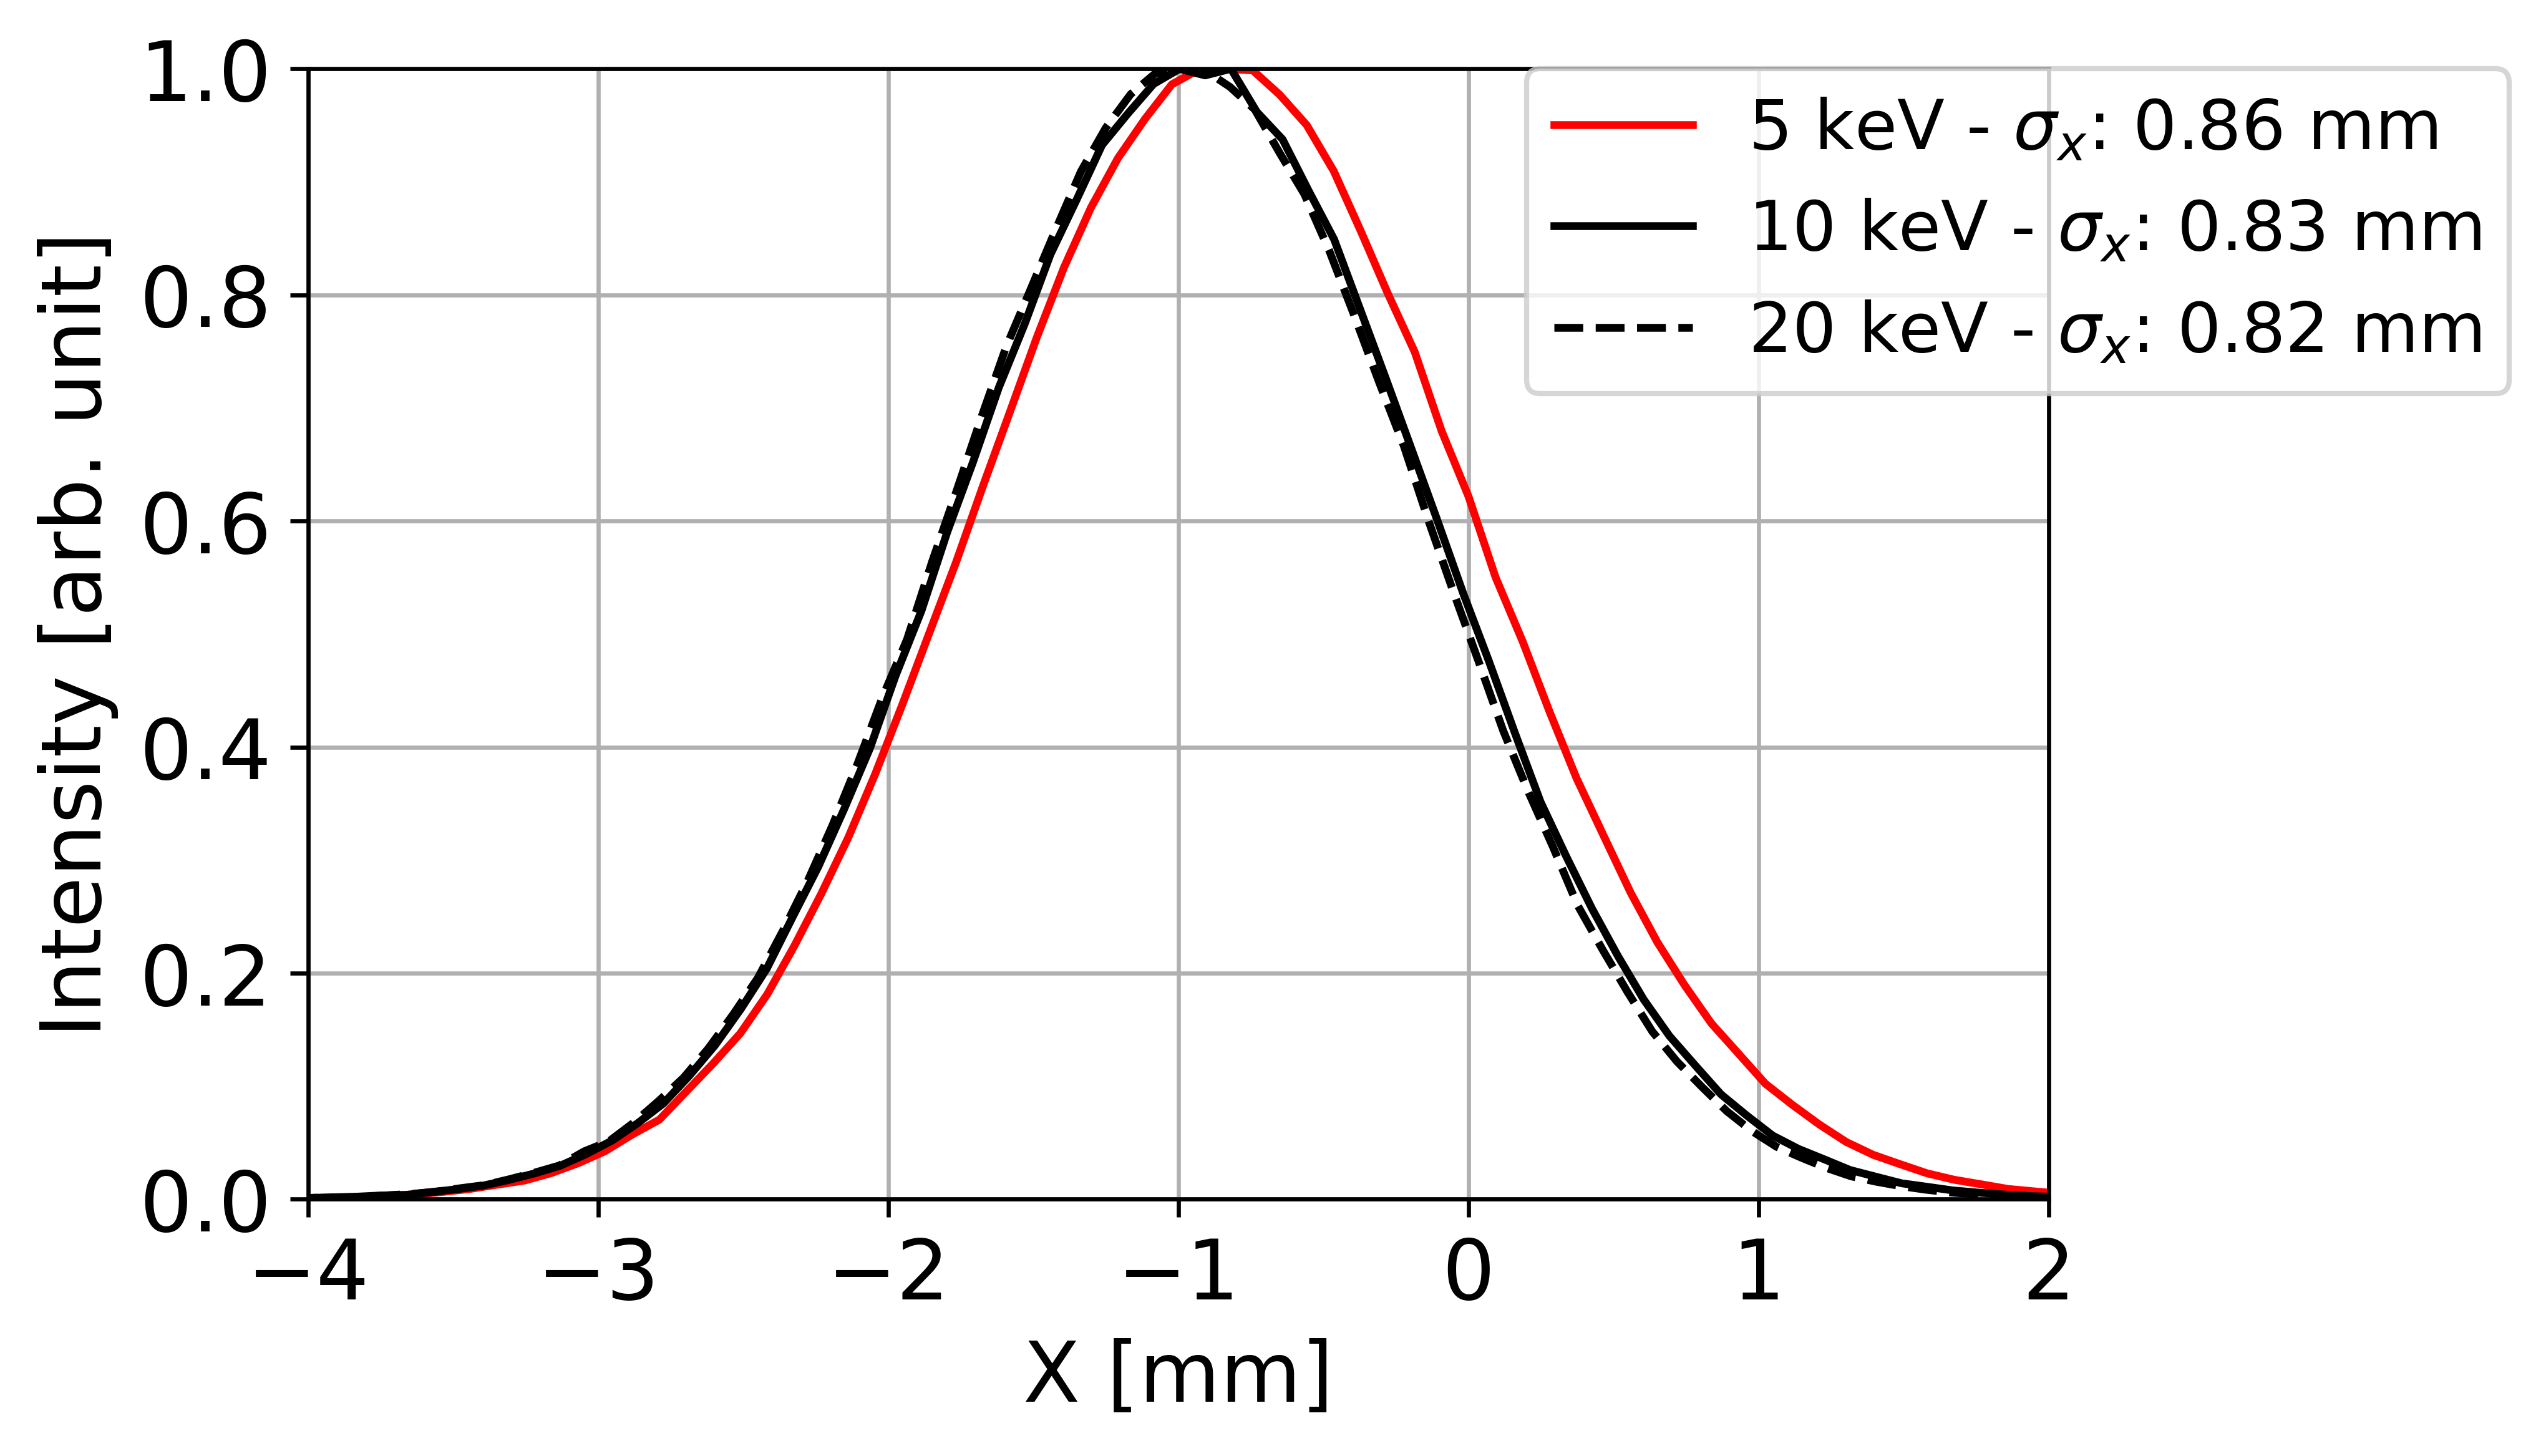
\includegraphics[width=\linewidth]{figures/beam_snapshots/3PW/sigmaX.png}
% \caption{Network 1}
\end{subfigure}
\hfill % maximize the horizontal distance between the graphs
\begin{subfigure}{0.45\textwidth}
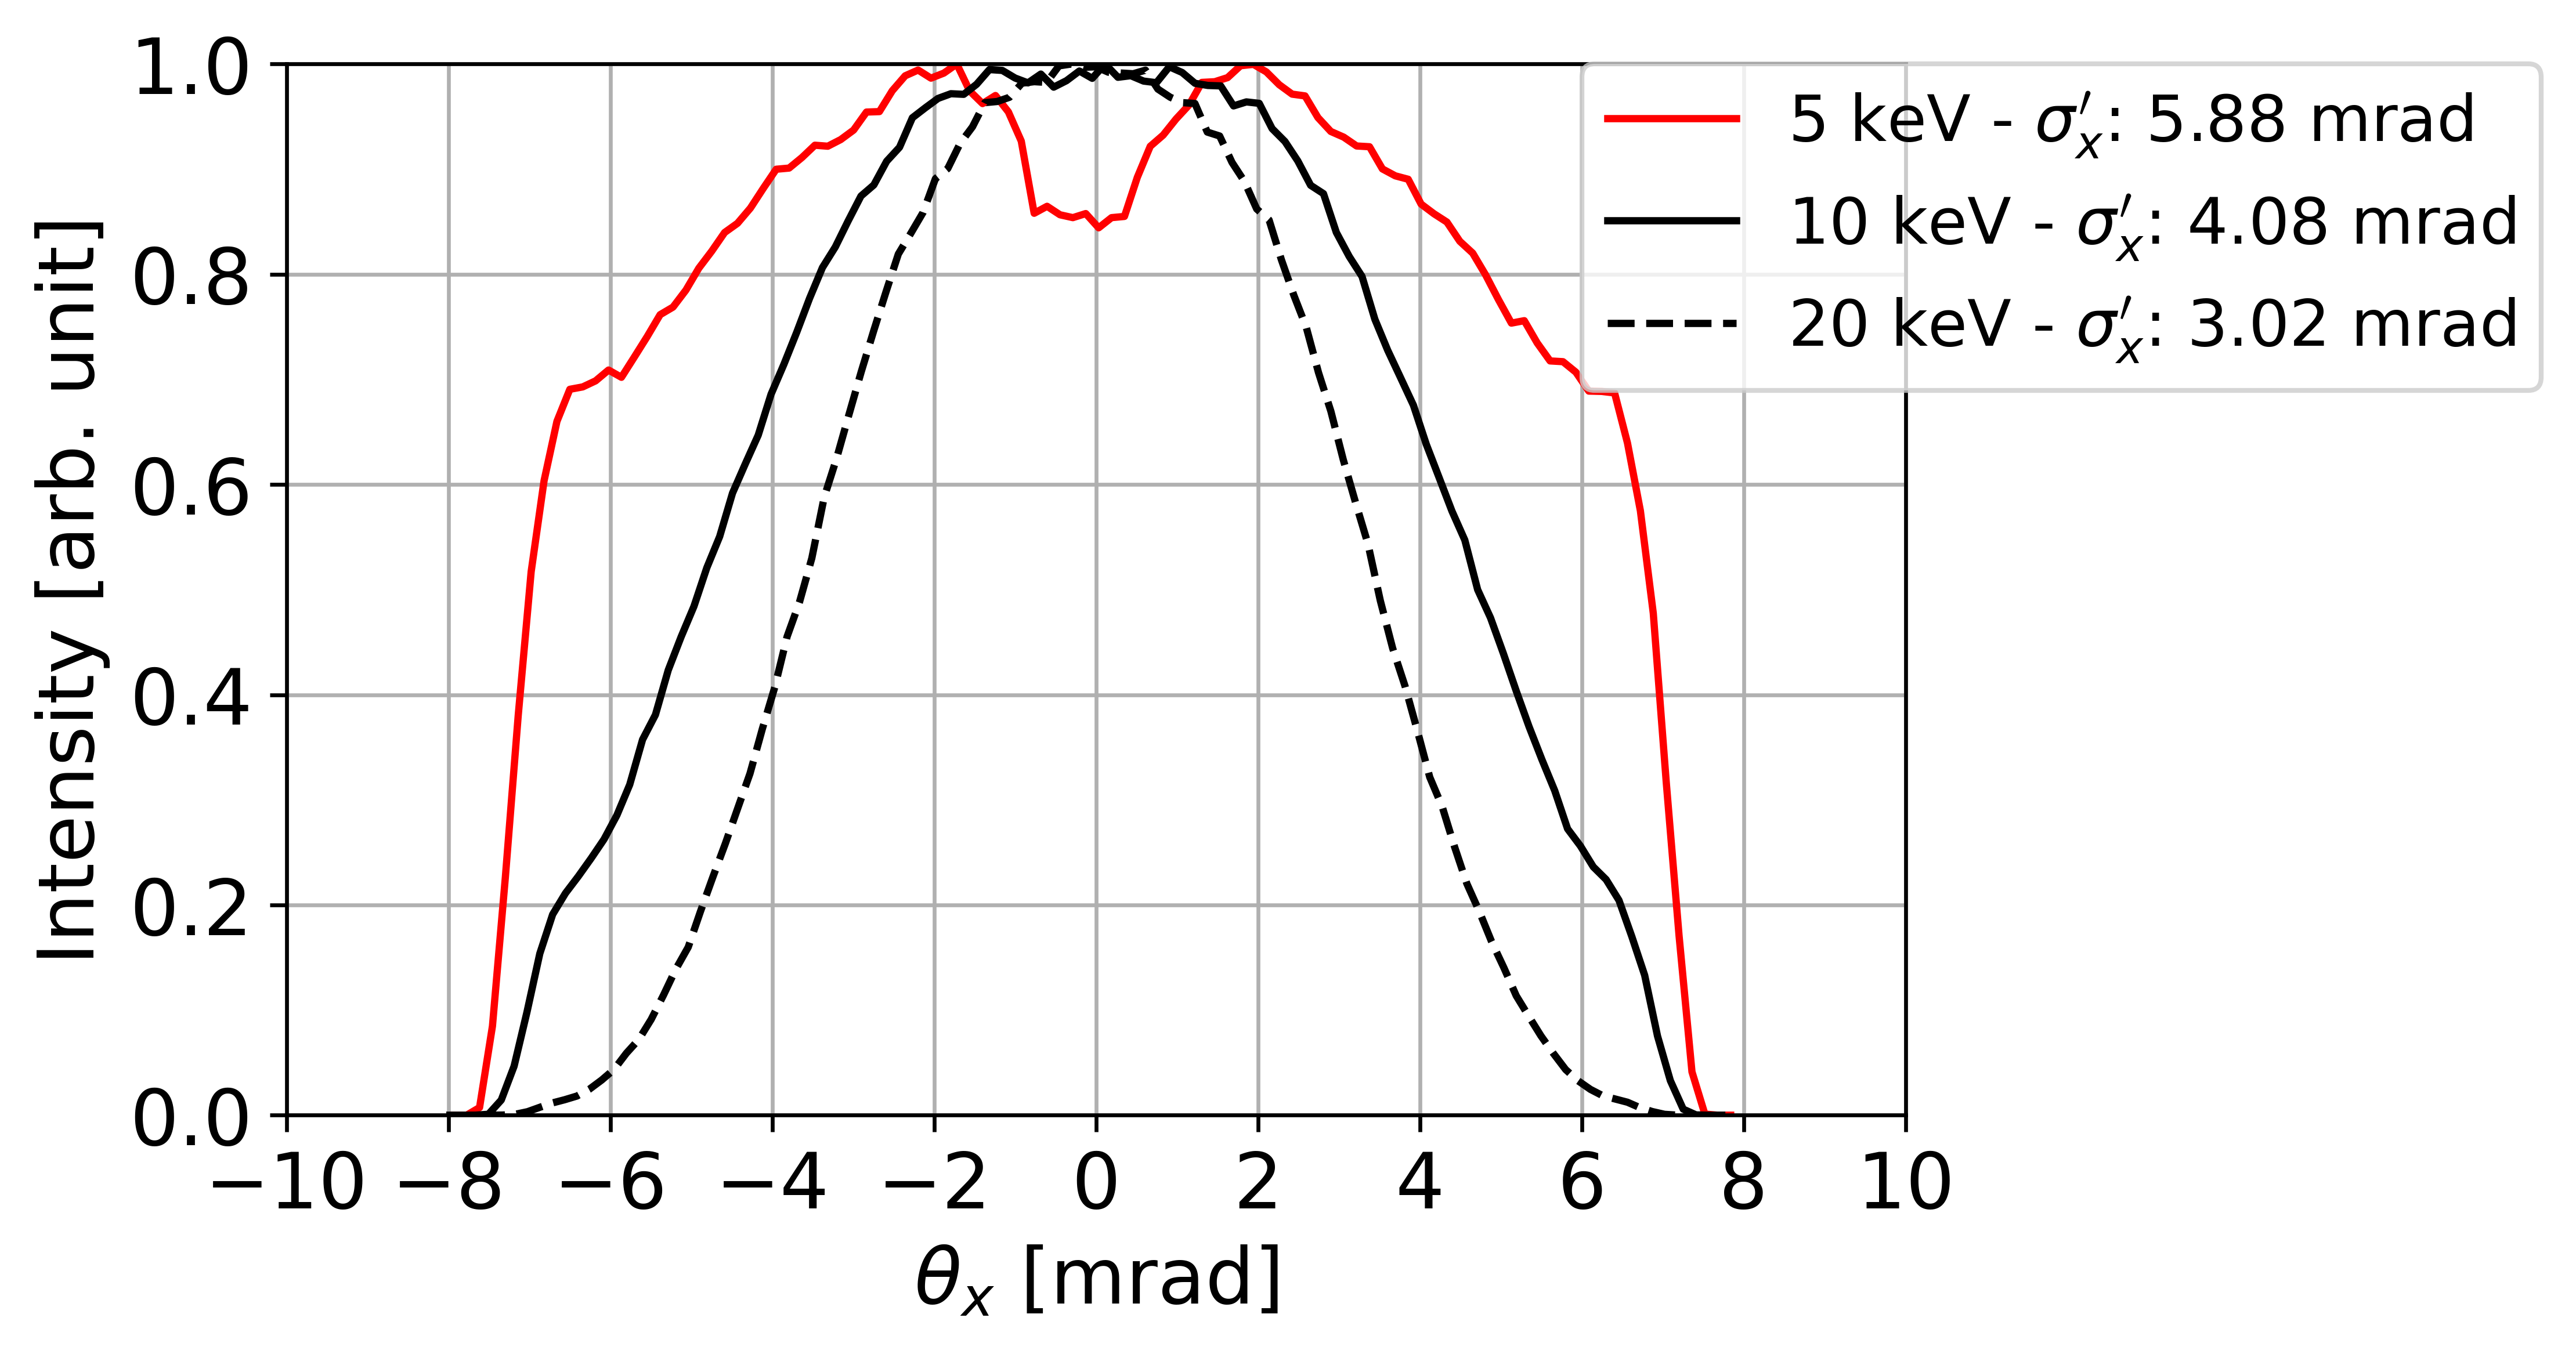
\includegraphics[width=\linewidth]{figures/beam_snapshots/3PW/sigmaXp.png}
% \caption{Network  2}
\end{subfigure}

\bigskip  % some extra vertical whitespace
\begin{subfigure}{0.45\textwidth}
\includegraphics[width=\linewidth]{c.pdf}
\caption{Network  3}
\end{subfigure}
\hfill % maximize the horizontal distance between the graphs
\begin{subfigure}{0.45\textwidth}
\includegraphics[width=\linewidth]{d.pdf}
\caption{Network  4}
\end{subfigure}

\caption{Averages and standard deviations} % Overall figure caption
\end{figure*}

For the power density of the input beam the contribution from two SESAME bending magnets (upstream and downstream of the ID) was considered in addition to the BEATS 3PW. The modified magnetic field profile used for the calculation is shown in Figure \ref{fig:modifiedfieldprofile}. \\
\begin{figure}[ht]
\centering
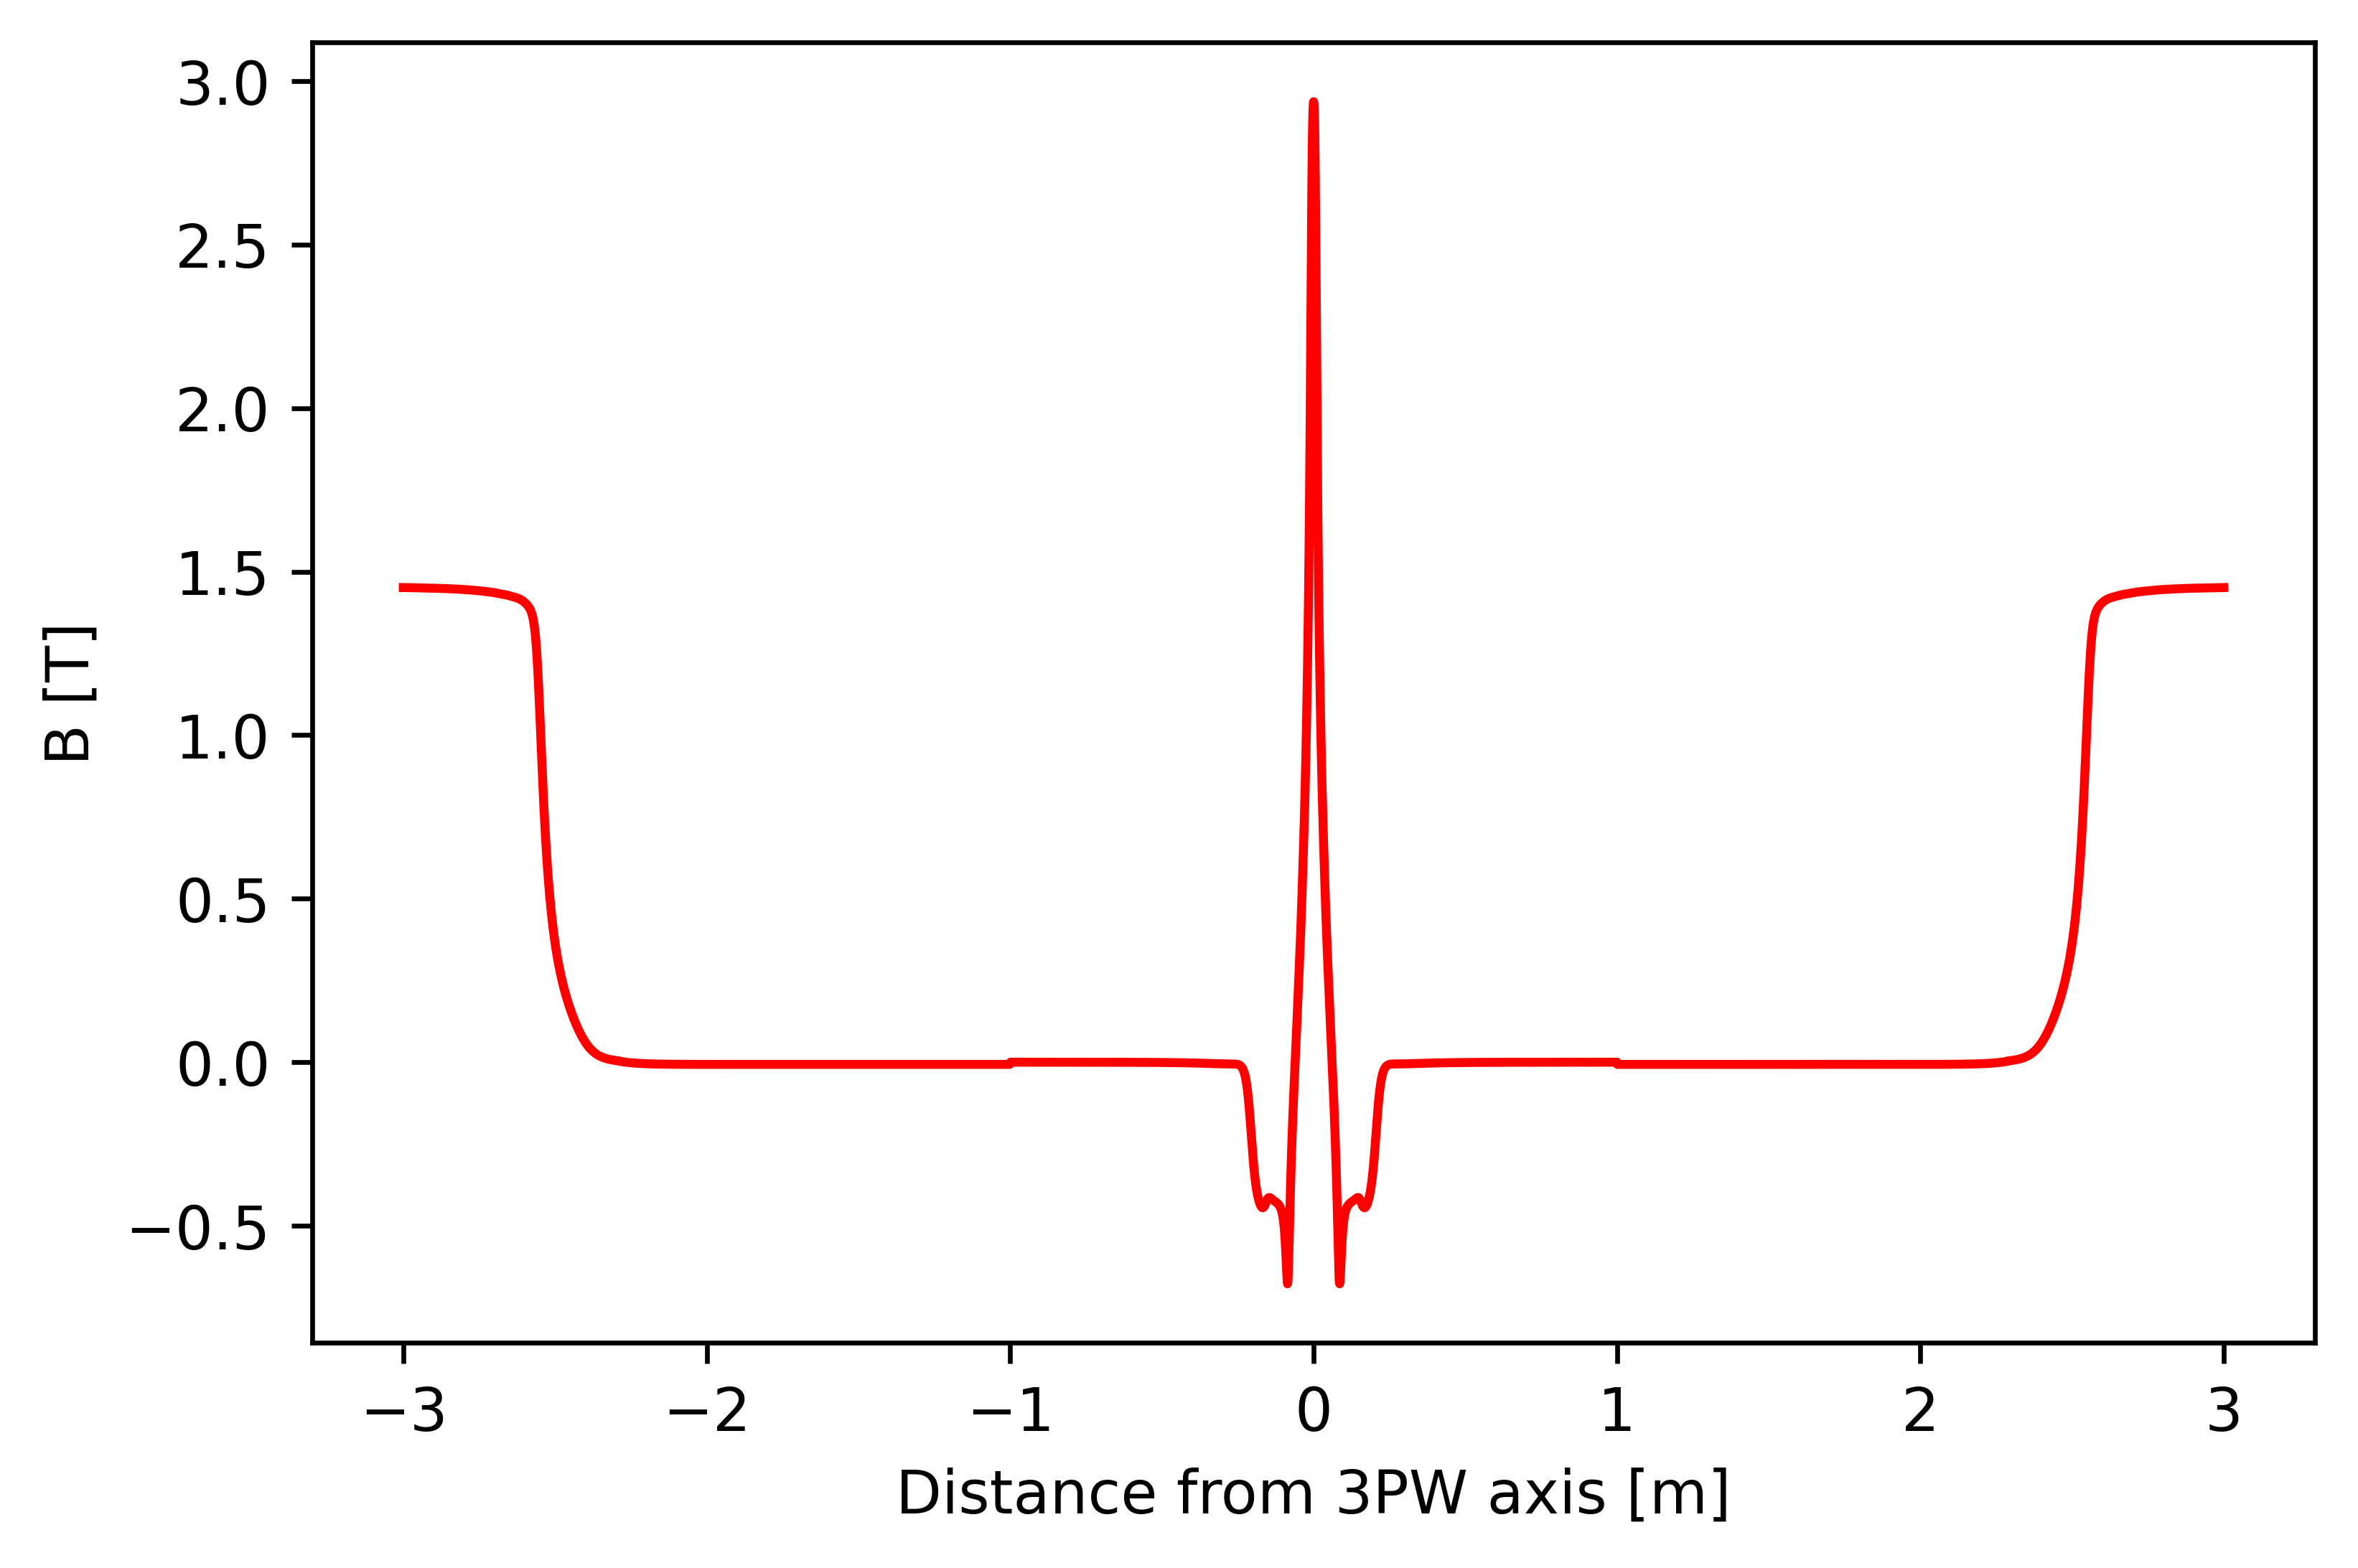
\includegraphics[width=0.8\textwidth]{images/modified_field_profile.png}
\caption{\label{fig:modifiedfieldprofile} Magnetic field profile modified considering the BEATS source plus two BMs (up and downstream) for calculation of the power load on the crotch absorber.}
\end{figure}
\section{Double Multilayer Monochromator (DMM)}
\subsection{Overview}

\begin{center}
\begin{tabular}[bhp]{|p{0.4\textwidth} | p{0.5\textwidth}|}
\hline
Deflection & Vertical \\
Distance from source (1st ML) & 15.165 m \\
Beamline aperture & 1.8 mrad × 0.4 mrad (Hor. × Ver.) \\
Beam size @ 1st mirror & 29 mm × 6 mm (Hor. × Ver.) \\
Working energy & 8 – 50 [keV] \\
ML length & 500 mm \\
Distance between MLs & 510 mm \\
Offset (variable) & Min. 4.2 – Max. 16.0 [mm] \\
Theta (Bragg angle) & -0.5 to +2.5 [deg] \\
Bragg resolution & 0.5 µrad \\
Max. power on 1st mirror & 133 W \\
Supplier & CINEL Strumenti Scientifici S.r.l. \\
\hline
\end{tabular}
\end{center}

\begin{figure}[ht]
\centering
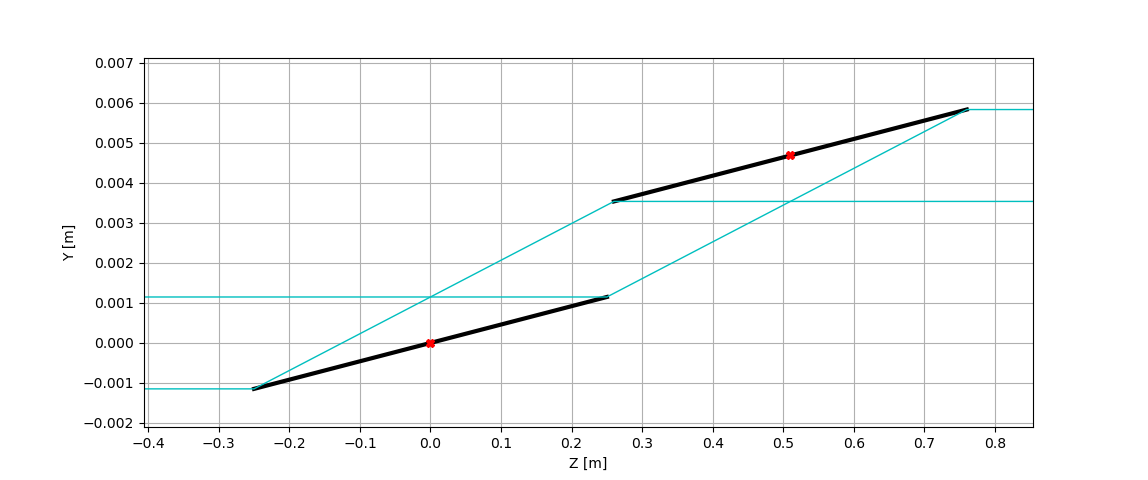
\includegraphics[width=0.8\textwidth]{./../figures/operation/DMM_mirrors_d3_E45_gr0.263_offset4.68.png}
\caption{\label{fig:DMM_mirrors_45keV} Mirrors position for d-spacing of 3 nm and 45 keV energy. Grazing angle: 0.263 deg. Offset: 4.68 mm.}
\end{figure}

%%%%%%%%%%%%%%%%%%%%%%%%%%%%%%%%%%%%%%%%%%%%%%%%%%%%%%%%%%%%%%%%%%%%%%%%%%%%%%%%%%%%
\subsection{Input beam}
A beam snapshot at 15.165 m from source is shown in Figure \ref{fig:snapshot_ML1}.
\begin{figure}[ht]
\centering
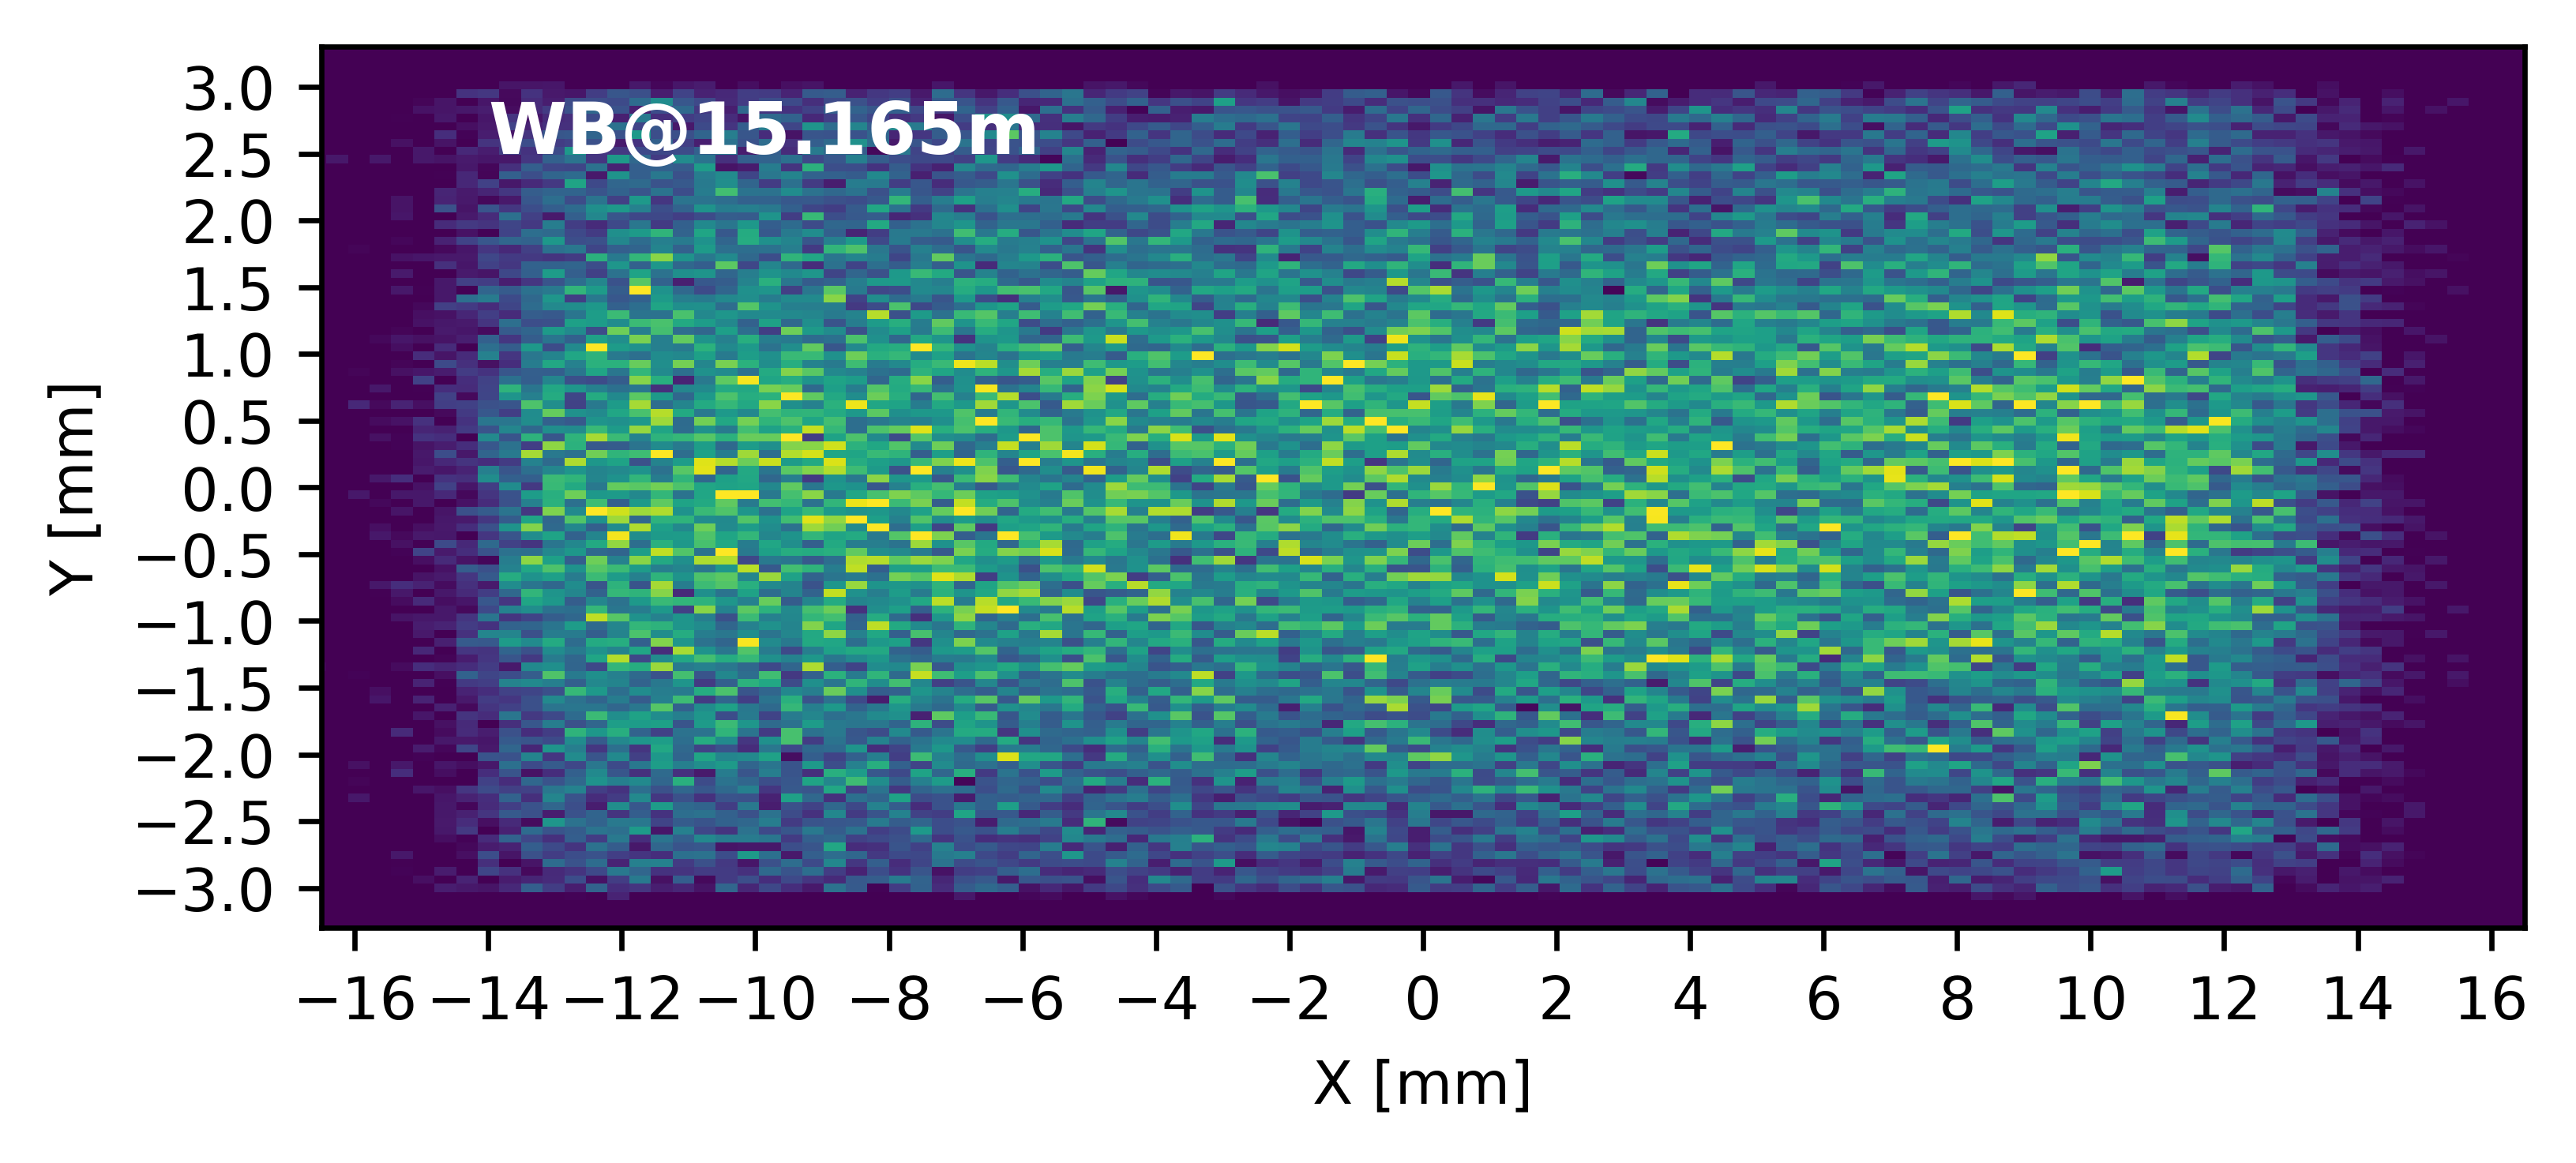
\includegraphics[width=0.8\textwidth]{./../../beam_snapshots/WB_snapshot_15.165.png}
\caption{\label{fig:snapshot_ML1} White beam snapshot at 15.165 m from source (center position of ML1).}
\end{figure}

\subsubsection{Power density}
The power density profile at 15.165 m from source is shown in Figure \ref{fig:power_profile_ML1}. Raw data can be found in the \powerprofilesurl. \\
\begin{figure}[ht]  % spans both columns
\begin{subfigure}{0.5\textwidth}
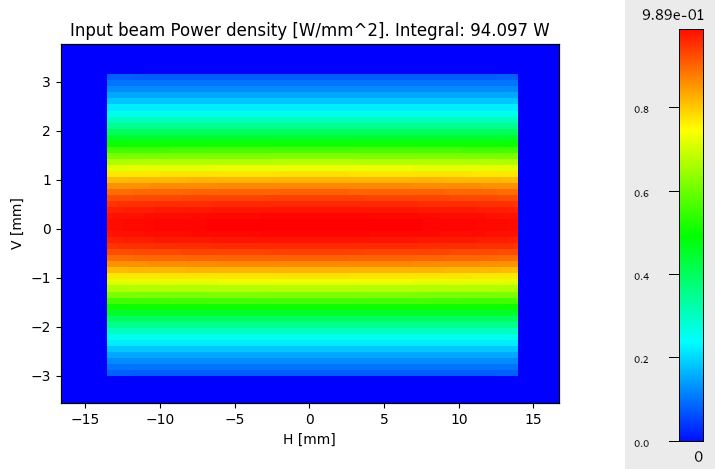
\includegraphics[width=\linewidth]{./../../power_profiles/power_profile_ML1.png}
% \caption{Network 1}
\end{subfigure}
\hfill % maximize the horizontal distance between the graphs
\begin{subfigure}{0.5\textwidth}
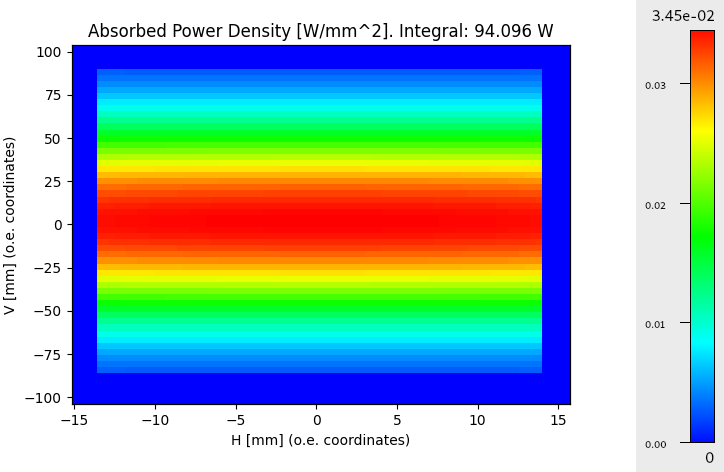
\includegraphics[width=\linewidth]{./../../power_profiles/power_profile_ML1_abs_2deg.png}
% \caption{Network  2}
\end{subfigure}
\caption{\label{fig:power_profile_ML1} Power density profile at 15.165 m from source (center position of ML1). (LEFT) Input beam. (RIGHT) Absorbed by substrate at maximum grazing (2 deg); reflectivity neglected. }
\end{figure}


%%%%%%%%%%%%%%%%%%%%%%%%%%%%%%%%%%%%%%%%%%%%%%%%%%%%%%%%%%%%%%%%%%%%%%%%%%%%%%%%%%%%
\subsection{ML coatings}
Following the increase in ML length to 500 mm the d-spacing of the high-energy stripe is changed back from 2.5 nm to 3.0 nm. This gives approx. +50\% int. reflectivity (dE/E increases from 2.3\% to 3.2\%). Thanks to the increased mirror length the whole vertical beam is intercepted even at min. grazing. \\
Coating specs of the two ML stripes are given in Table \ref{tab:coatings}.
\begin{center}
\begin{tabular}[bhp]{|p{0.4\textwidth} | p{0.3\textwidth} | p{0.3\textwidth} |}
\hline
 & \textbf{STRIPE 1} & \textbf{STRIPE 2} \\
 & \textbf{$[W/B_{4}C]_{100} - d 3.0 nm $} & \textbf{$[Ru/B_{4}C]_{65} - d 4.0 nm $} \\
\hline
\label{tab:coatings}
\end{tabular}
\end{center}

%%%%%%%%%%%%%%%%%%%%%%%%%%%%%%%%%%%%%%%%%%%%%%%%%%%%%%%%%%%%%%%%%%%%%%%%%%%%%%%%%%%%
\subsection{Substrates}
The ML length was increased to 500 mm. A drawing of the substrate size proposed by CINEL is attached.

\begin{center}
\begin{tabular}[bhp]{|p{0.4\textwidth} | p{0.5\textwidth}|}
\hline
Substrate dimension & 500 mm × 70 mm × 60 mm \\
 & (drawing BEATS_DMM_ML_400mm_2 attached) \\
Coated area & 500 mm × 25 mm (2 stripes) \\
Surface roughness & < 0.3 nm rms \\
Slope error along Z & ≤ 0.3 µrad rms \\
Slope error along X & < 20 µrad rms \\
\hline
\end{tabular}
\end{center}


%%%%%%%%%%%%%%%%%%%%%%%%%%%%%%%%%%%%%%%%%%%%%%%%%%%%%%%%%%%%%%%%%%%%%%%%%%%%%%%%%%%%
\subsection{Substrates slope error}
For this paragraph a substrate length of 500 mm is considered.

\subsubsection{Raytracing}
\begin{wrapfigure}{r}{0.3\linewidth}
\centering
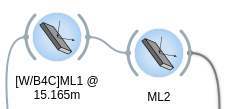
\includegraphics[width=0.3\textwidth]{images/DMM_oasys.png}
\caption{\label{fig:DMM_oasys} Double Multilayer Monochromator in Oasys Shadow.}
\end{wrapfigure}

The double-bounce DMM is modelled with two Shadow Plane Mirror widgets in series (Figure \ref{fig:DMM_oasys}). ML reflectivity is modelled with a Shadow PreMLayer widget as shown in Figure \ref{fig:PreMLayer}. The mirror surface is modified with Surface Error external splines with varying longitudinal slope error (0.1, 0.2, 0.3, 0.4 and 0.5 $\mu rad$ RMS). These modified surfaces (\ref{fig:fractals}) are simulated with the Shadow PreProcessor - Height Profile Simulator widget. The transversal slope error is kept constant at 20 $\mu rad$ RMS and fractal profiles are chosen. 

\begin{figure}  % spans both columns
\begin{subfigure}{0.5\textwidth}
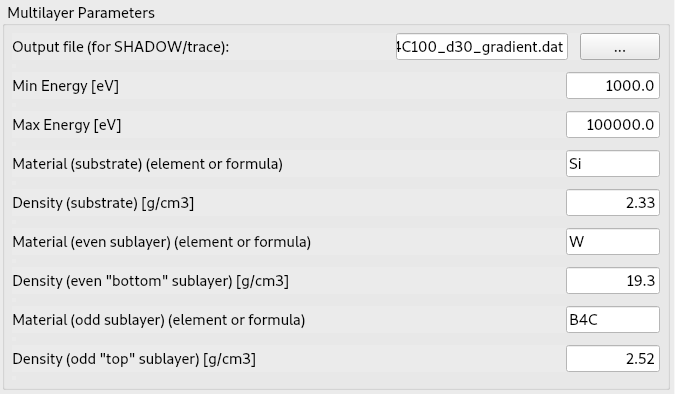
\includegraphics[width=\linewidth]{images/MLspecs_a.png}
\end{subfigure}
\hfill % maximize the horizontal distance between the graphs
\begin{subfigure}{0.5\textwidth}
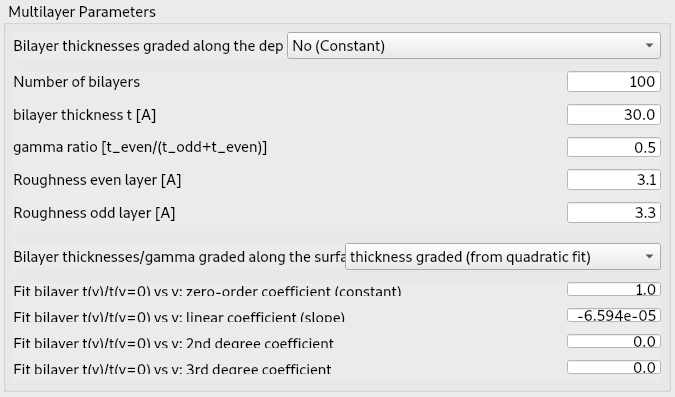
\includegraphics[width=\linewidth]{images/MLspecs_b.png}
\end{subfigure}
\caption{\label{fig:PreMLayer} PreMLayer widget settings in Shadow. }
\end{figure}

\begin{figure}[!htb]
\minipage{0.32\textwidth}
  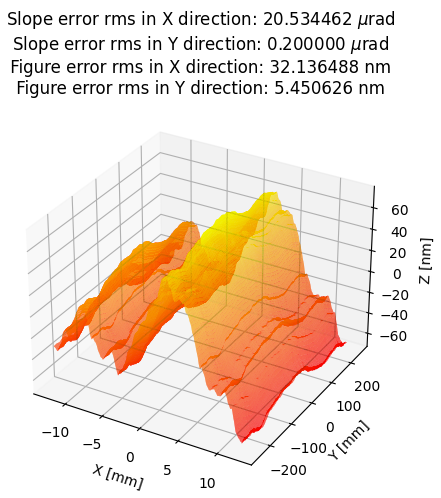
\includegraphics[width=\linewidth]{./../figures/slope_error/surface_error_profile_500x25_02x20urad.png}
  % \caption{A really Awesome Image}\label{fig:awesome_image1}
\endminipage\hfill
\minipage{0.32\textwidth}
  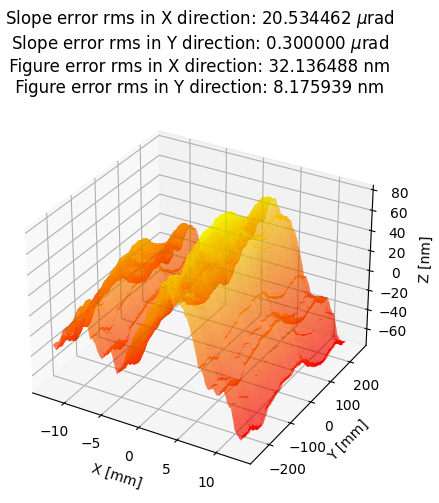
\includegraphics[width=\linewidth]{./../figures/slope_error/surface_error_profile_500x25_03x20urad.png}
  % \caption{A really Awesome Image}\label{fig:awesome_image2}
\endminipage\hfill
\minipage{0.32\textwidth}%
  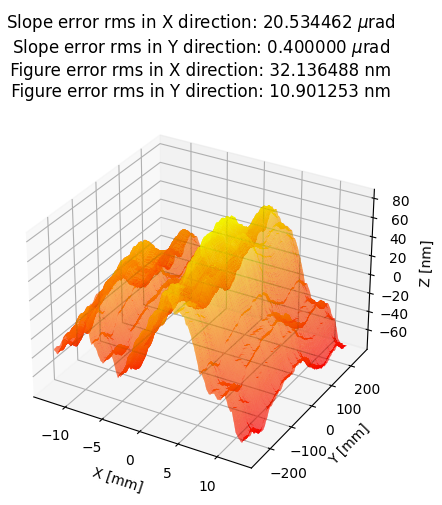
\includegraphics[width=\linewidth]{./../figures/slope_error/surface_error_profile_500x25_04x20urad.png}
  %\caption{A really Awesome Image}\label{fig:awesome_image3}
\endminipage
\caption{\label{fig:fractals} Modified mirror surfaces. }
\end{figure}

%%%%%%%%%%%%%%%%%%%%%%%%%%%%%%%%%%%%%%%%%%%%%%%%%%%%%%%%%%%%%%%%%%%%%%%%%%%%%%%%%%
\clearpage
\subsubsection{0.1 urad}
\begin{figure}[H]
\centering
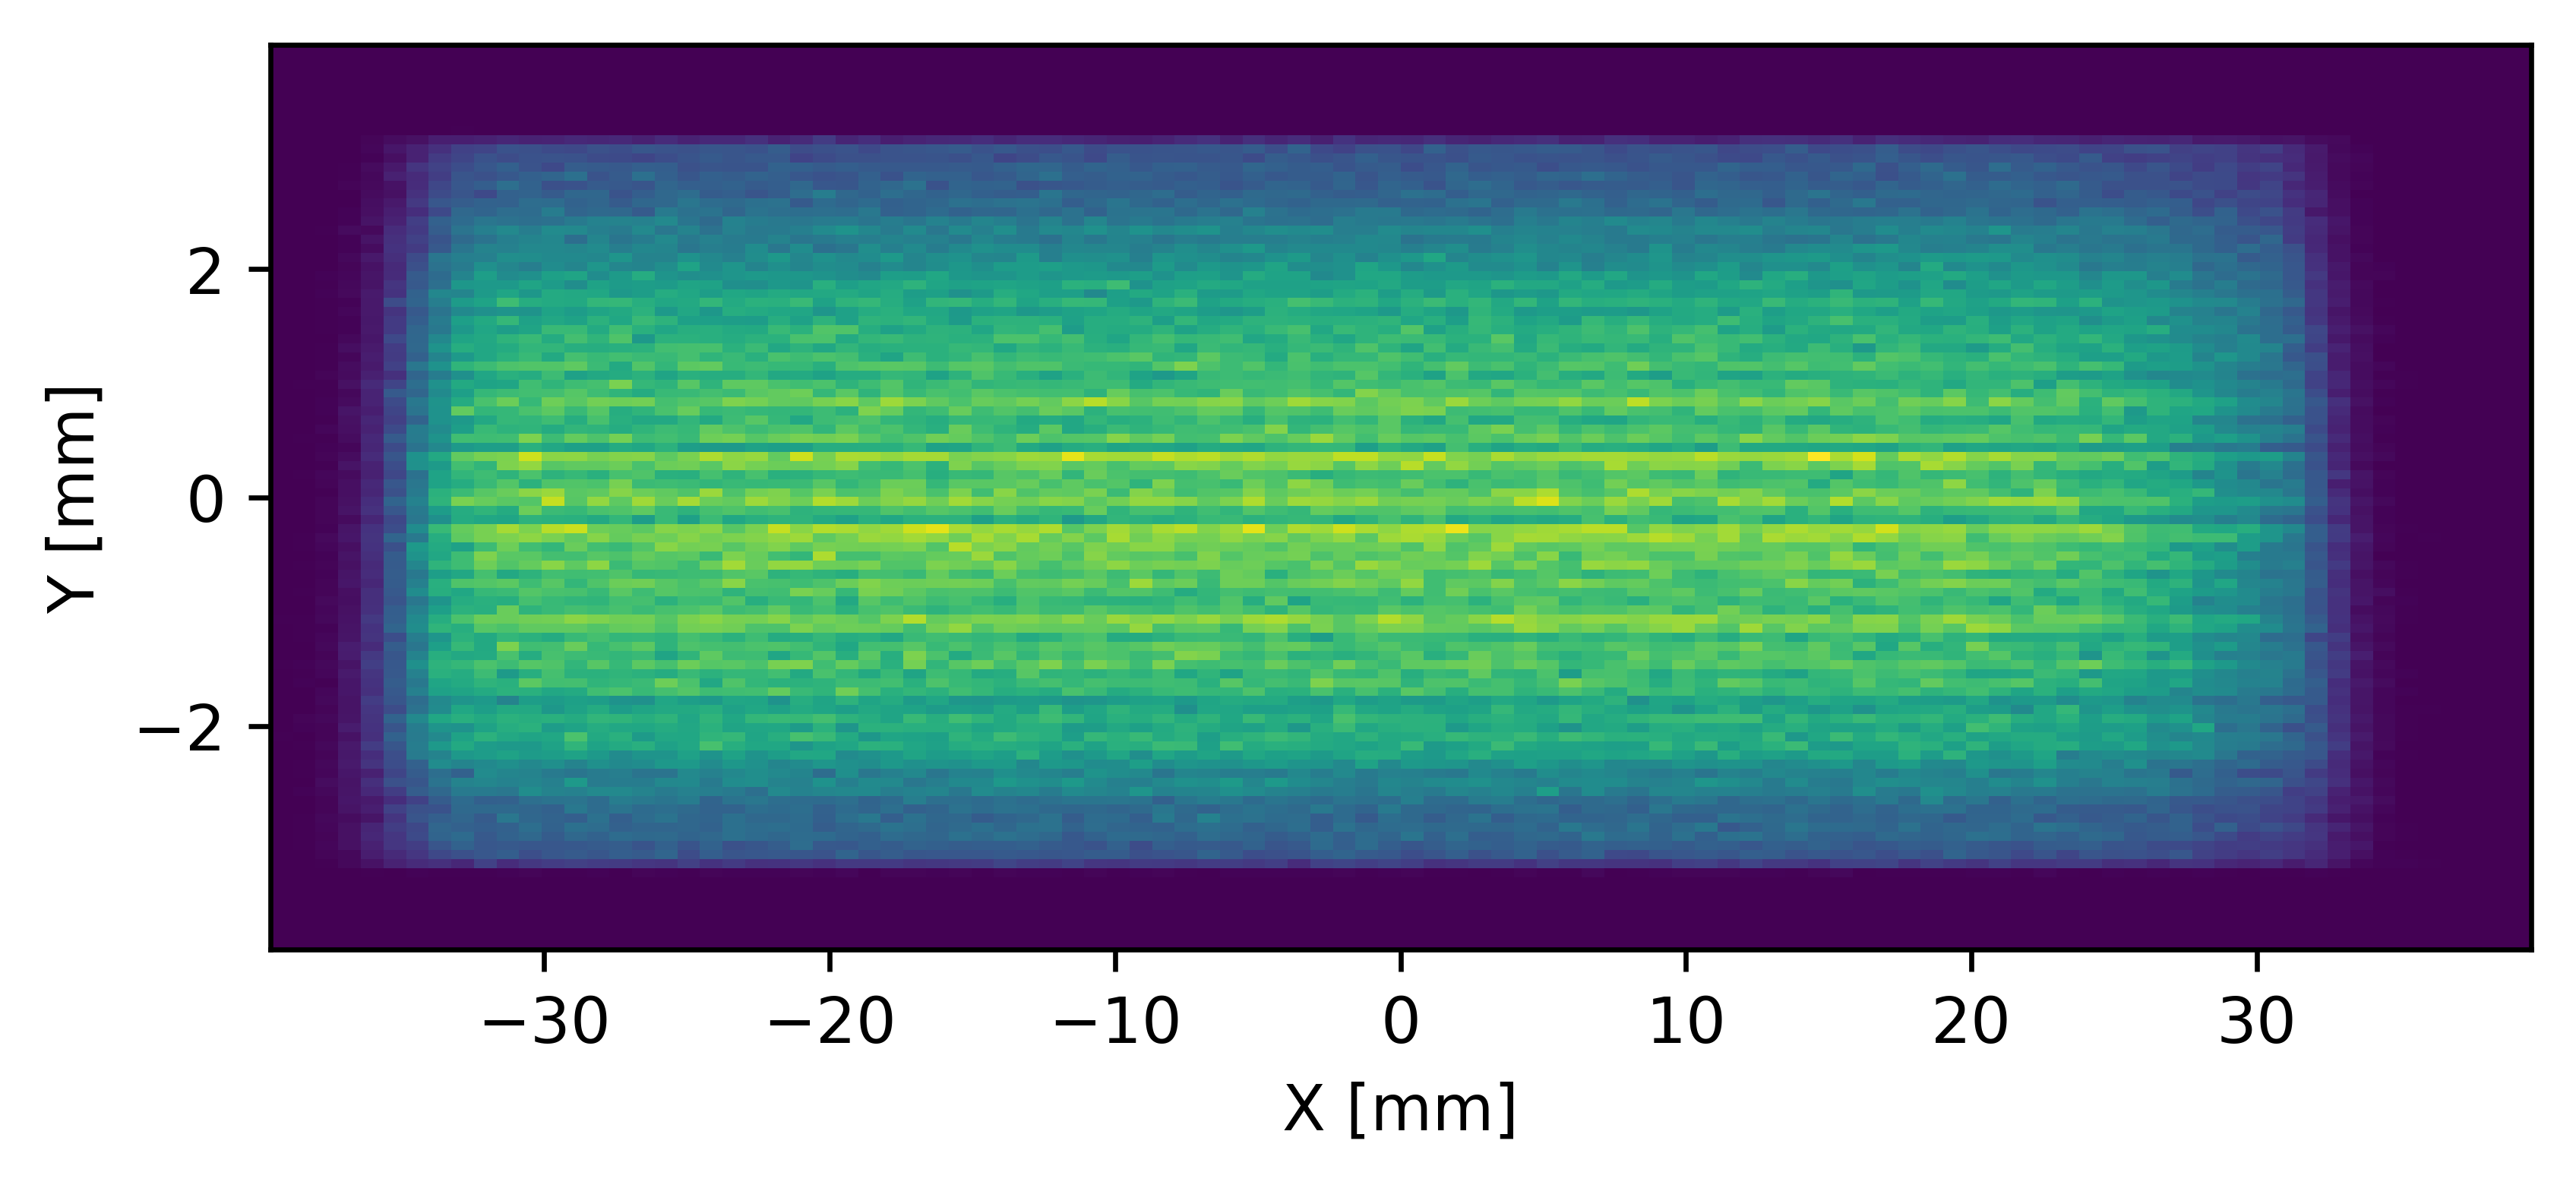
\includegraphics[width=0.9\linewidth]{./../figures/slope_error/WB4C_d30_d-spacing_gradient_45keV_slope_error01urad.png}
\end{figure}

\begin{figure}[H]
\centering
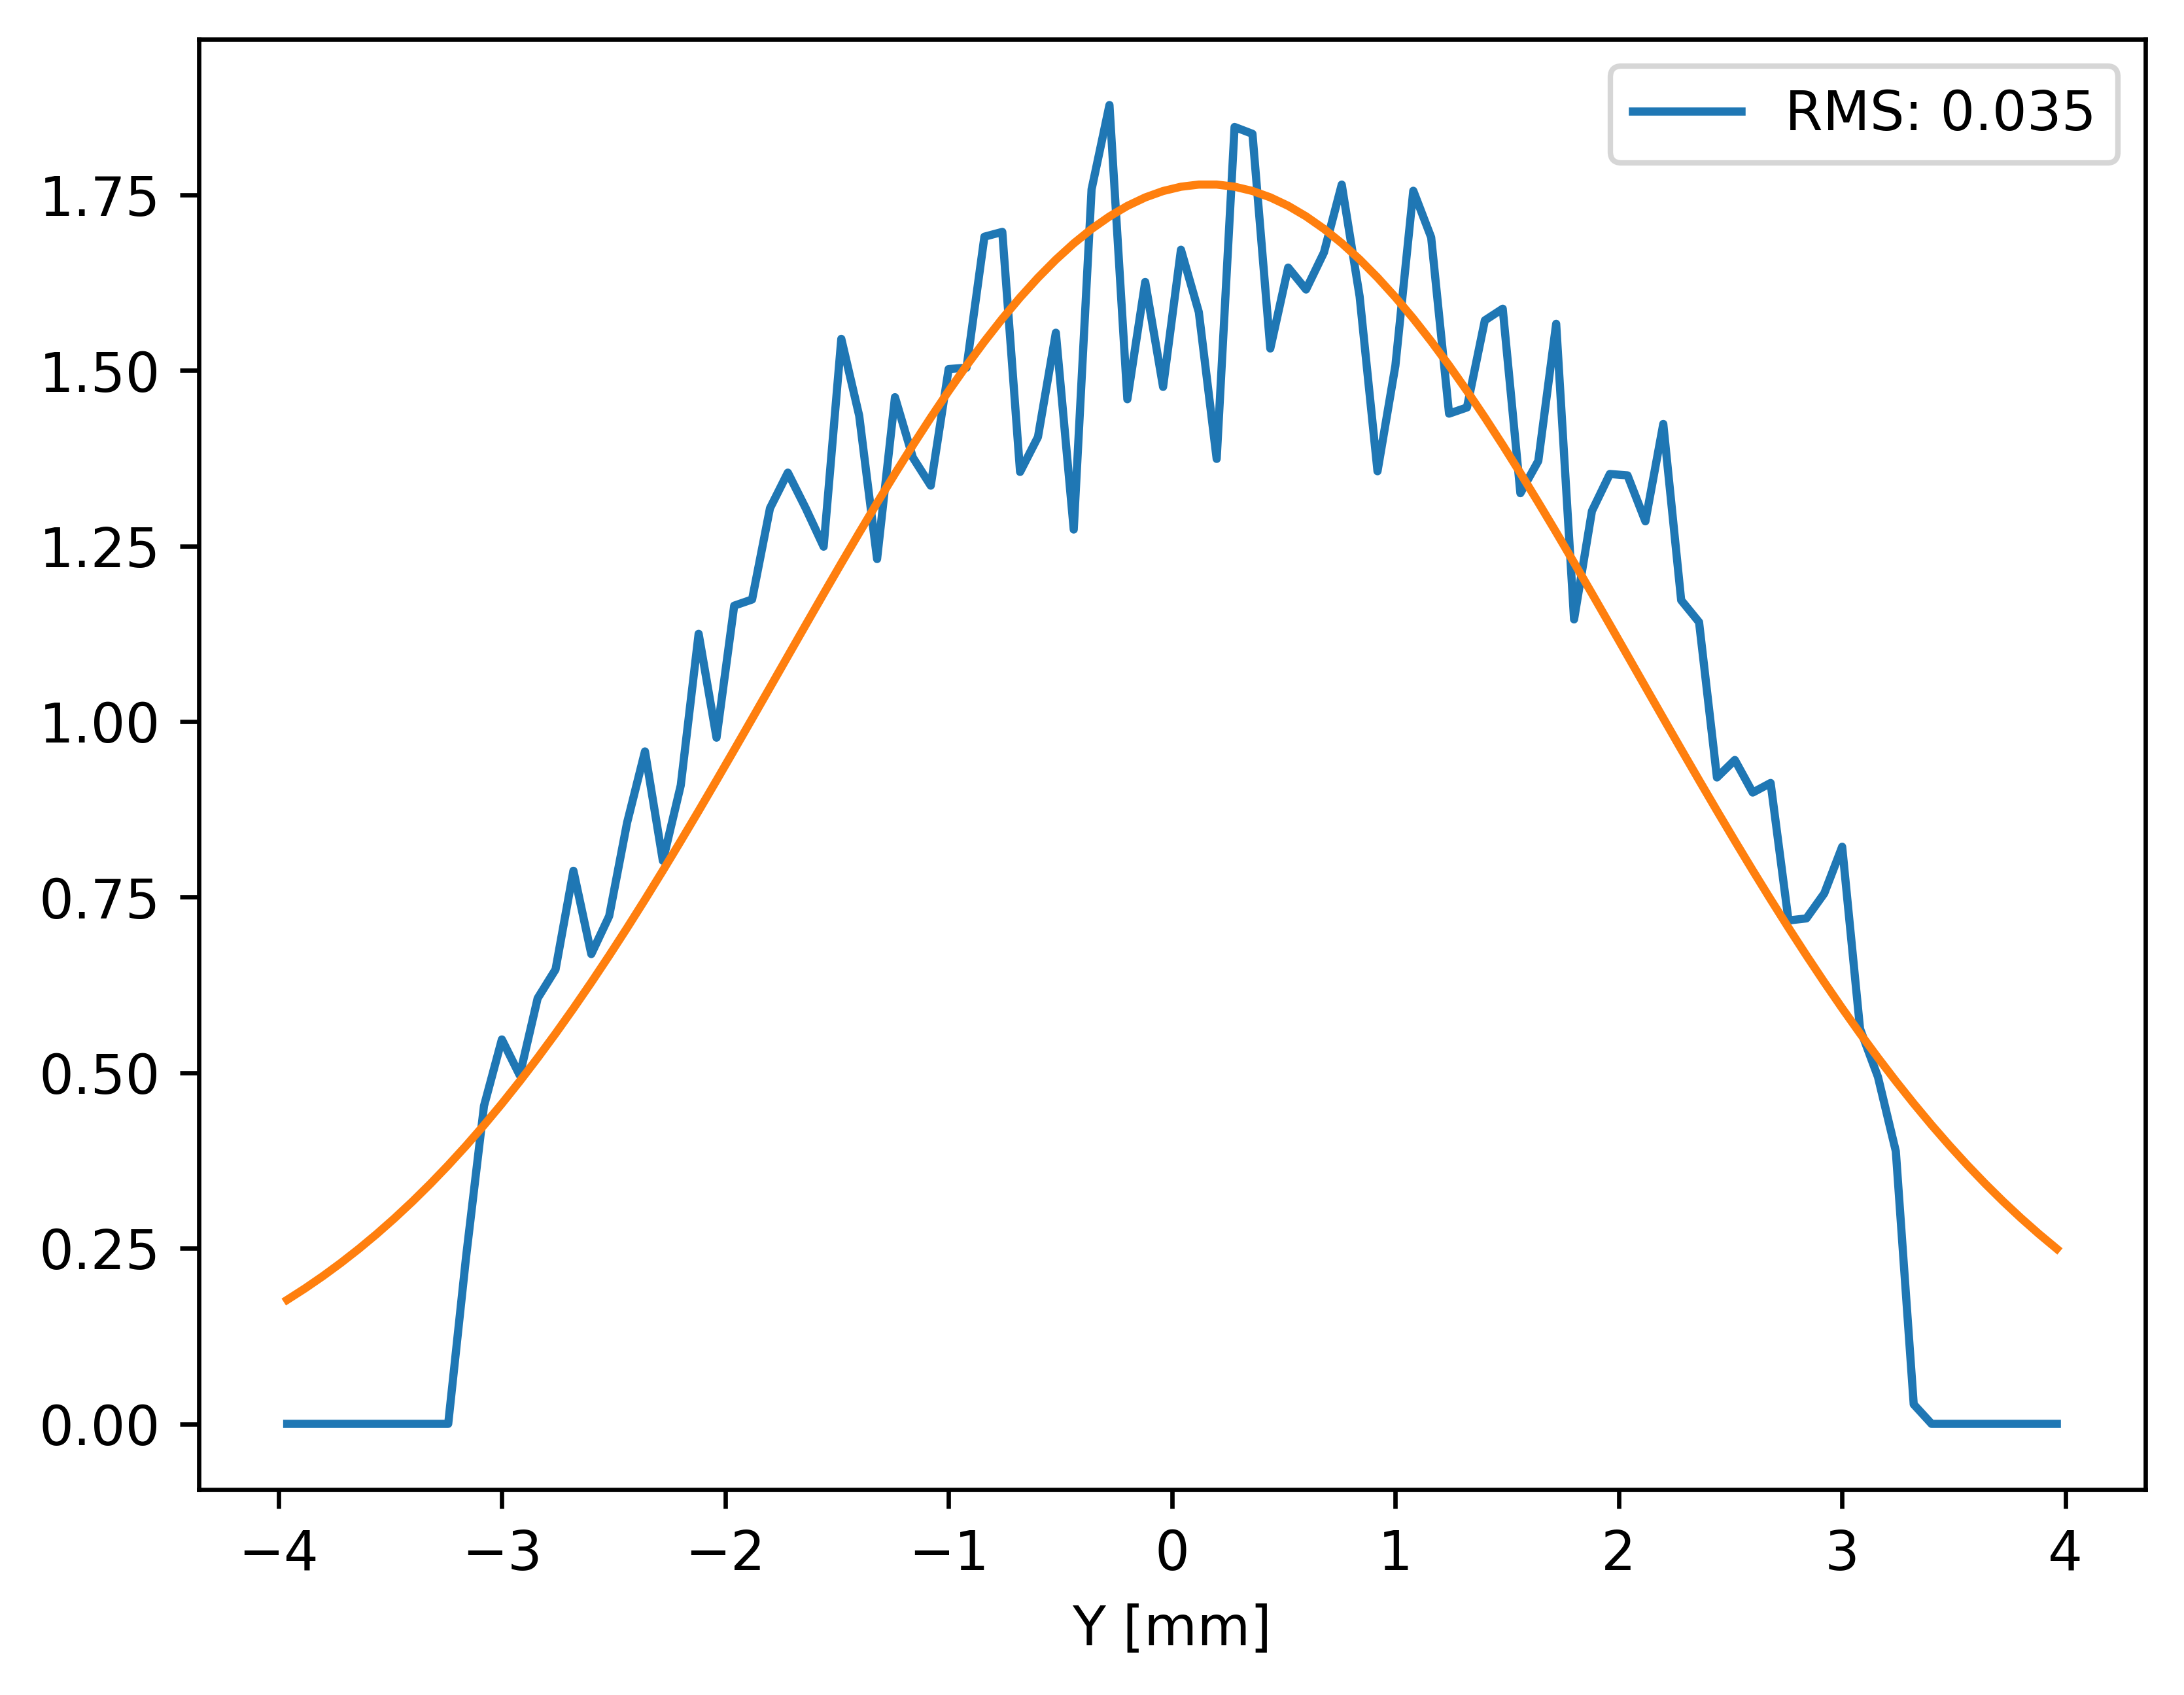
\includegraphics[width=0.9\linewidth]{./../figures/slope_error/WB4C_d30_d-spacing_gradient_45keV_slope_error01urad_Yprofile.png}
\caption{0.1 urad}
\label{fig:01urad}
\end{figure}

%%%%%%%%%%%%%%%%%%%%%%%%%%%%%%%%%%%%%%%%%%%%%%%%%%%%%%%%%%%%%%%%%%%%%%%%%%%%%%%%%%
\clearpage
\subsubsection{0.2 urad}
\begin{figure}[H]
\centering
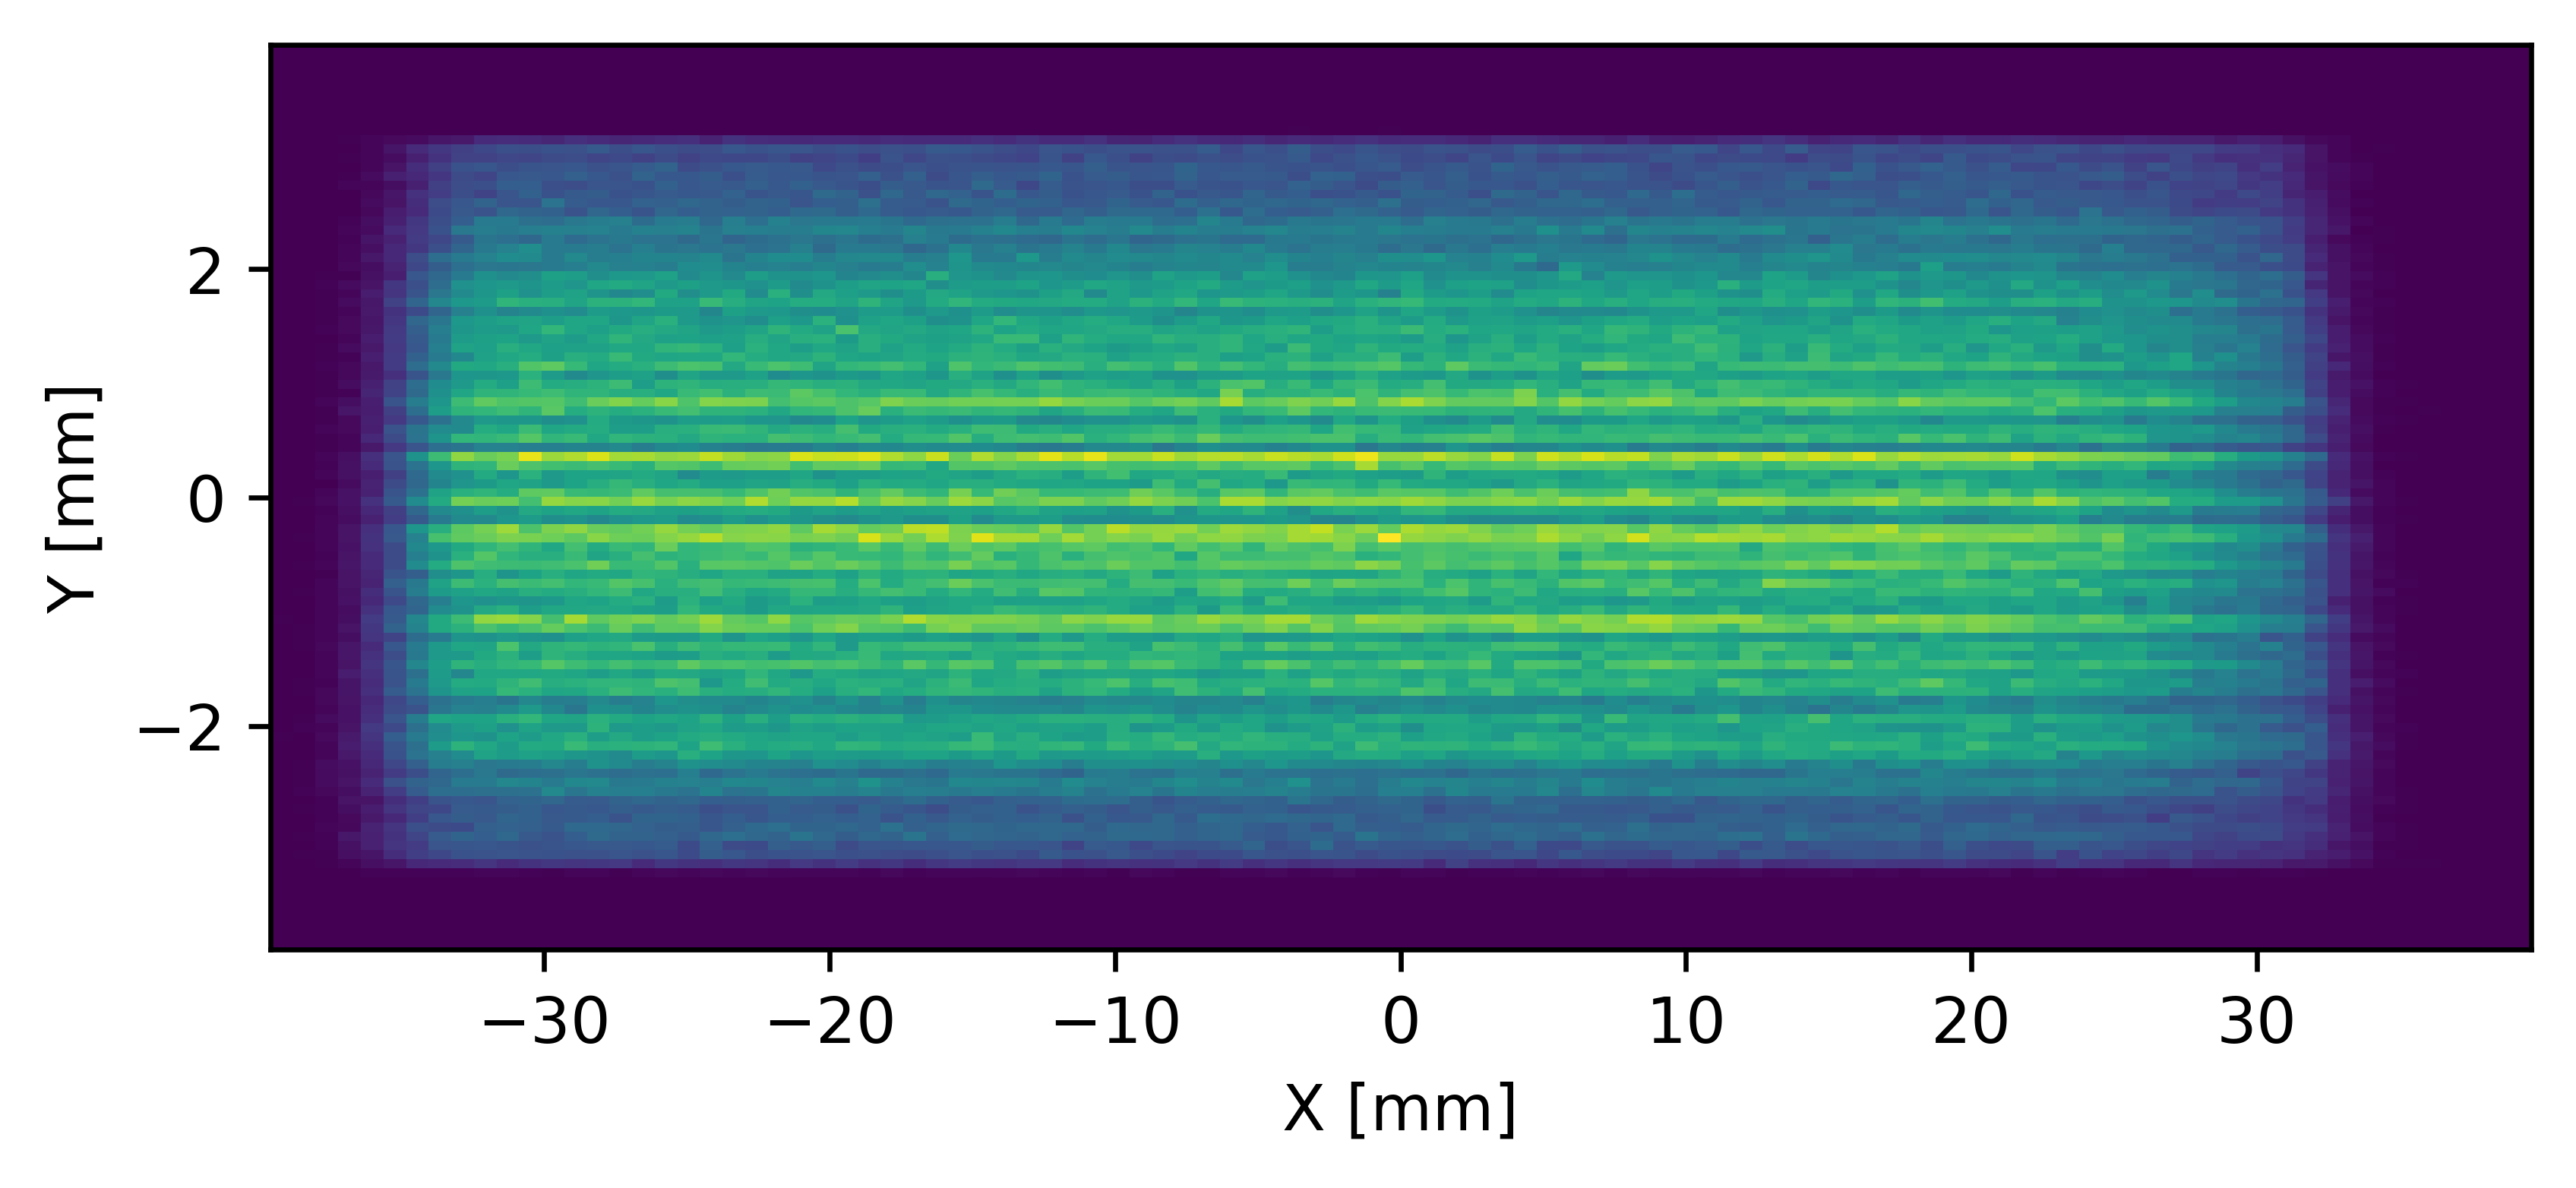
\includegraphics[width=0.9\linewidth]{./../figures/slope_error/WB4C_d30_d-spacing_gradient_45keV_slope_error02urad.png}
\end{figure}

\begin{figure}[H]
\centering
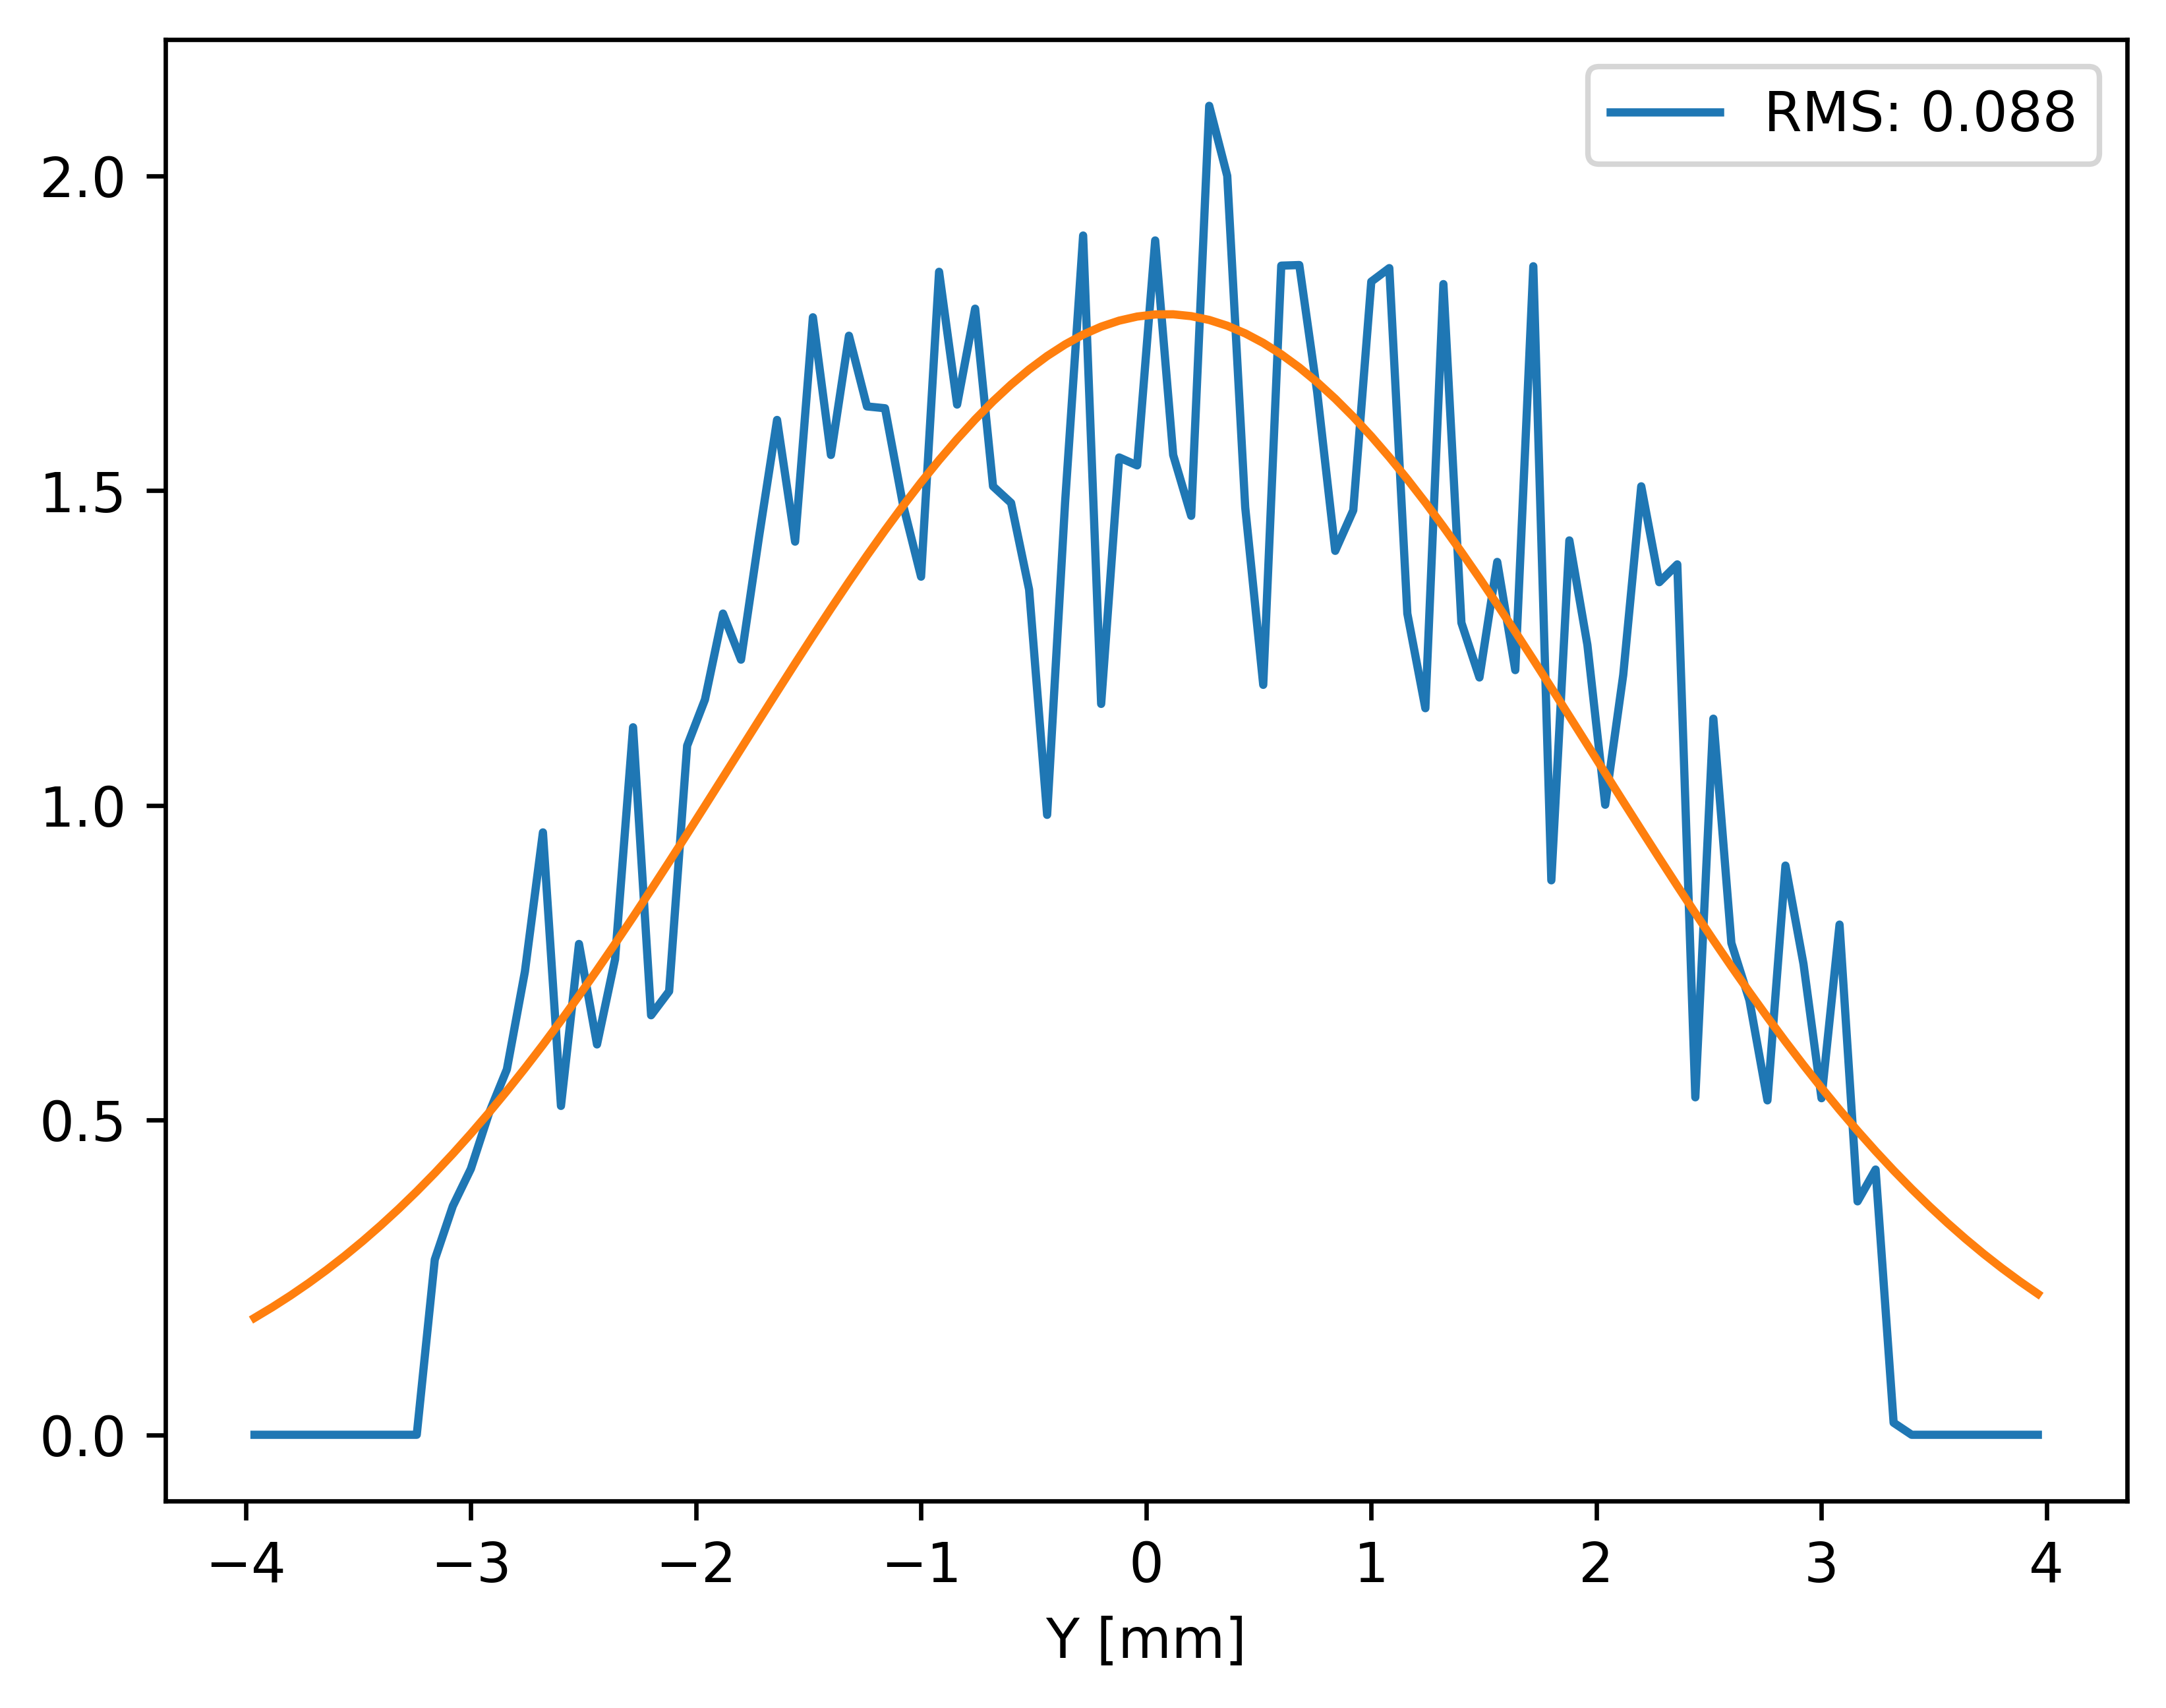
\includegraphics[width=0.9\linewidth]{./../figures/slope_error/WB4C_d30_d-spacing_gradient_45keV_slope_error02urad_Yprofile.png}
\caption{0.2 urad}
\label{fig:02urad}
\end{figure}

%%%%%%%%%%%%%%%%%%%%%%%%%%%%%%%%%%%%%%%%%%%%%%%%%%%%%%%%%%%%%%%%%%%%%%%%%%%%%%%%%%
\clearpage
\subsubsection{0.25 urad}
\begin{figure}[H]
\centering
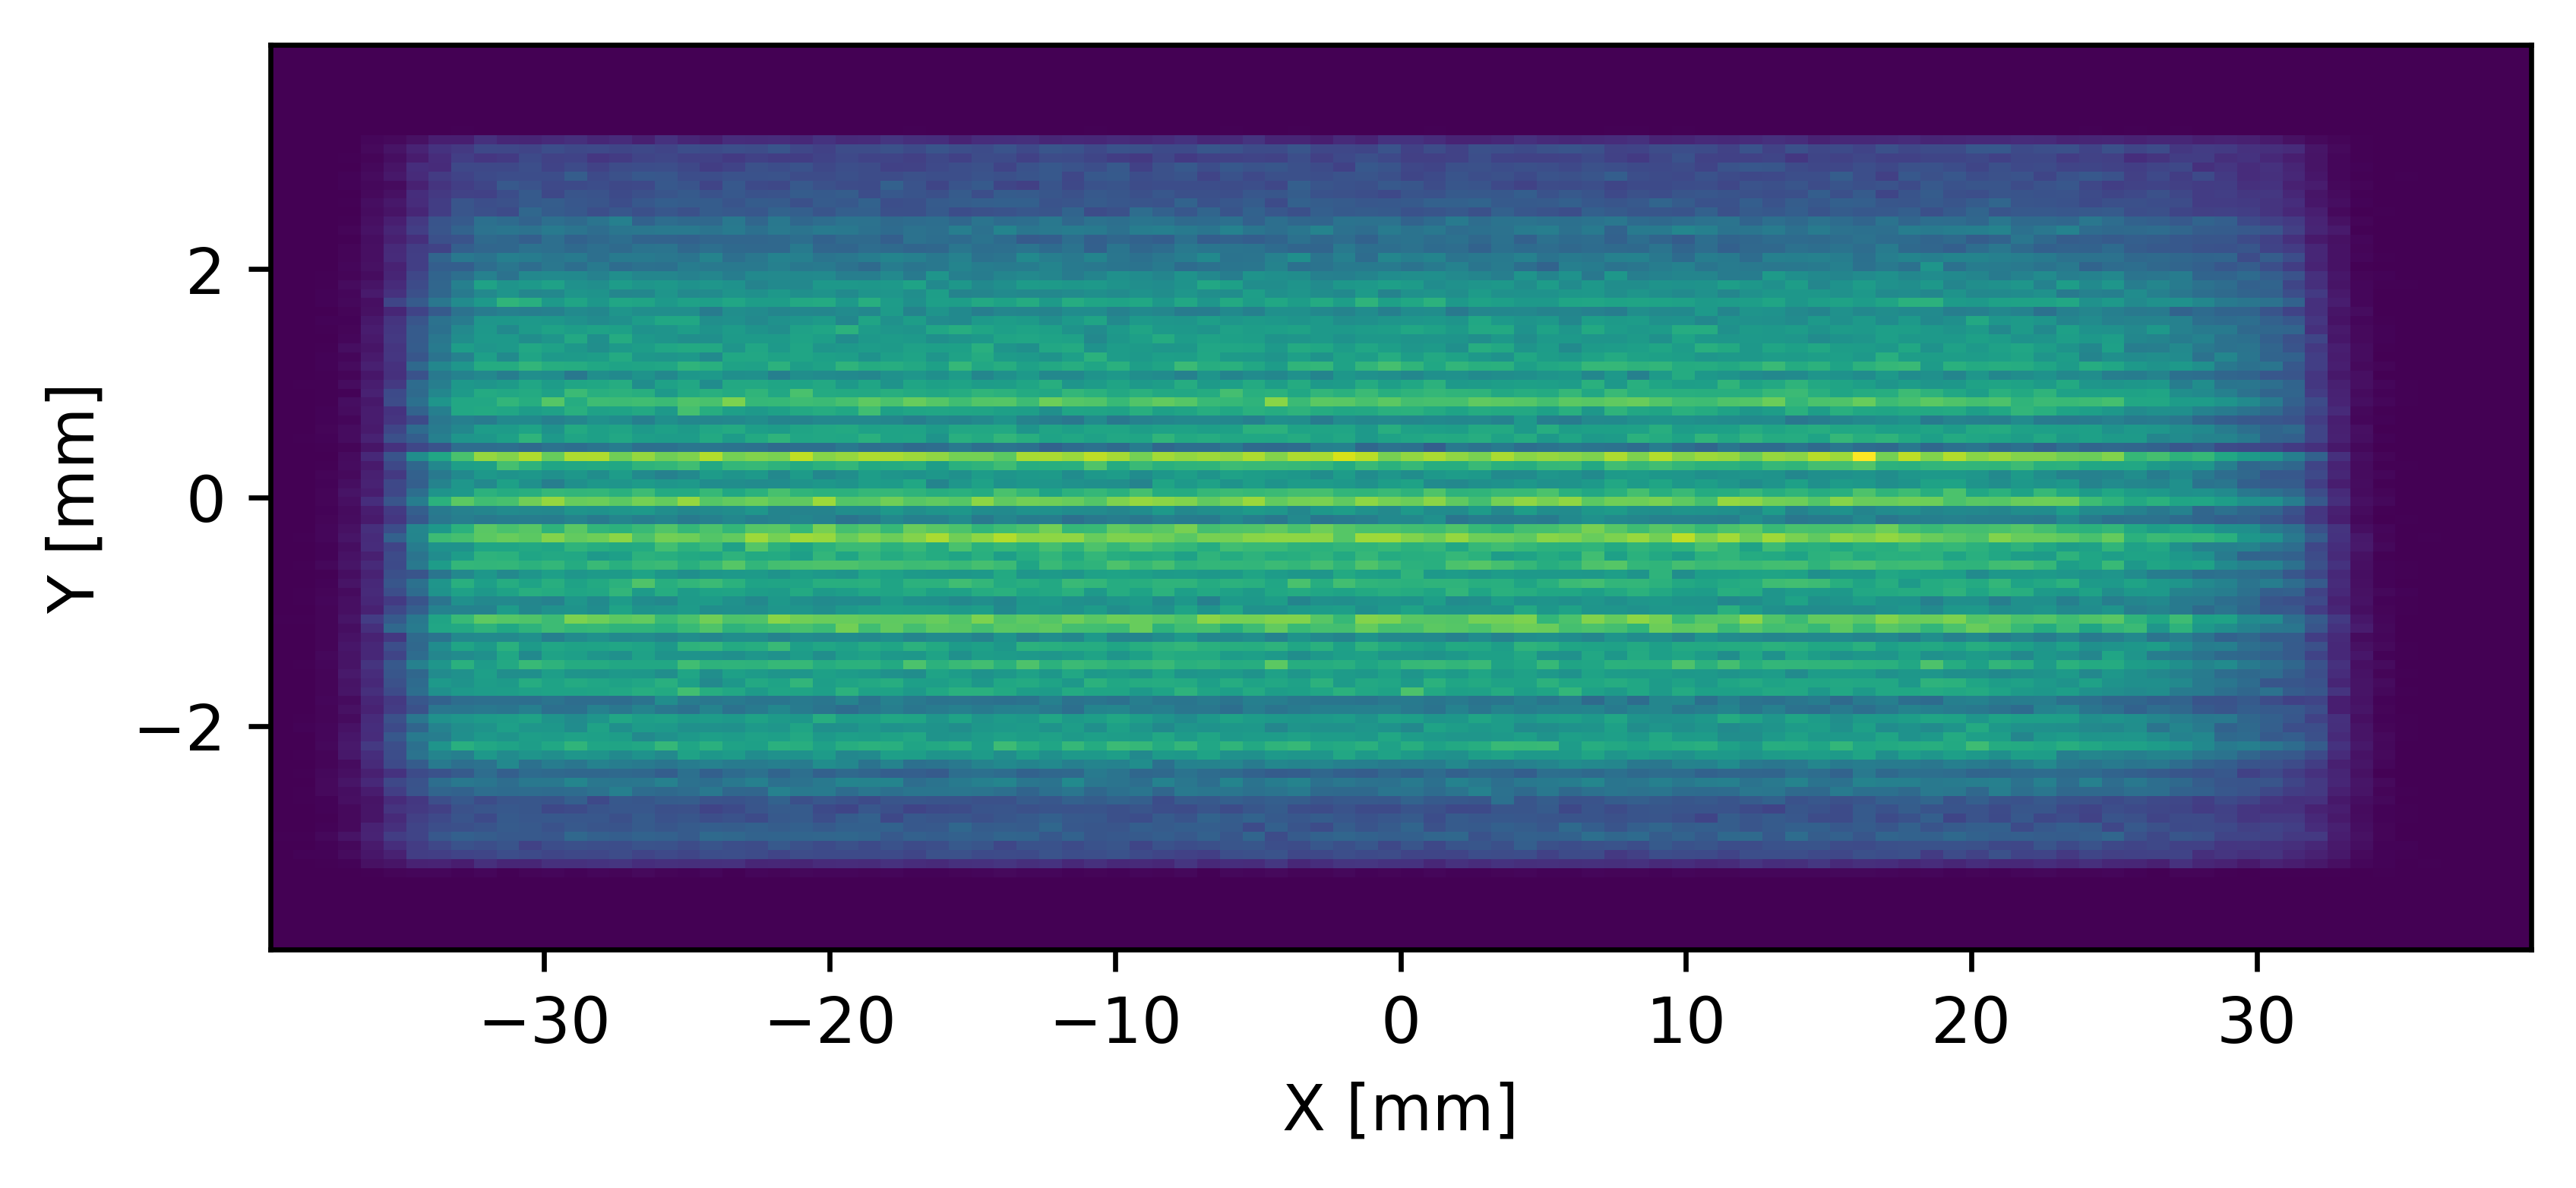
\includegraphics[width=0.9\linewidth]{./../figures/slope_error/WB4C_d30_d-spacing_gradient_45keV_slope_error025urad.png}
\end{figure}

\begin{figure}[H]
\centering
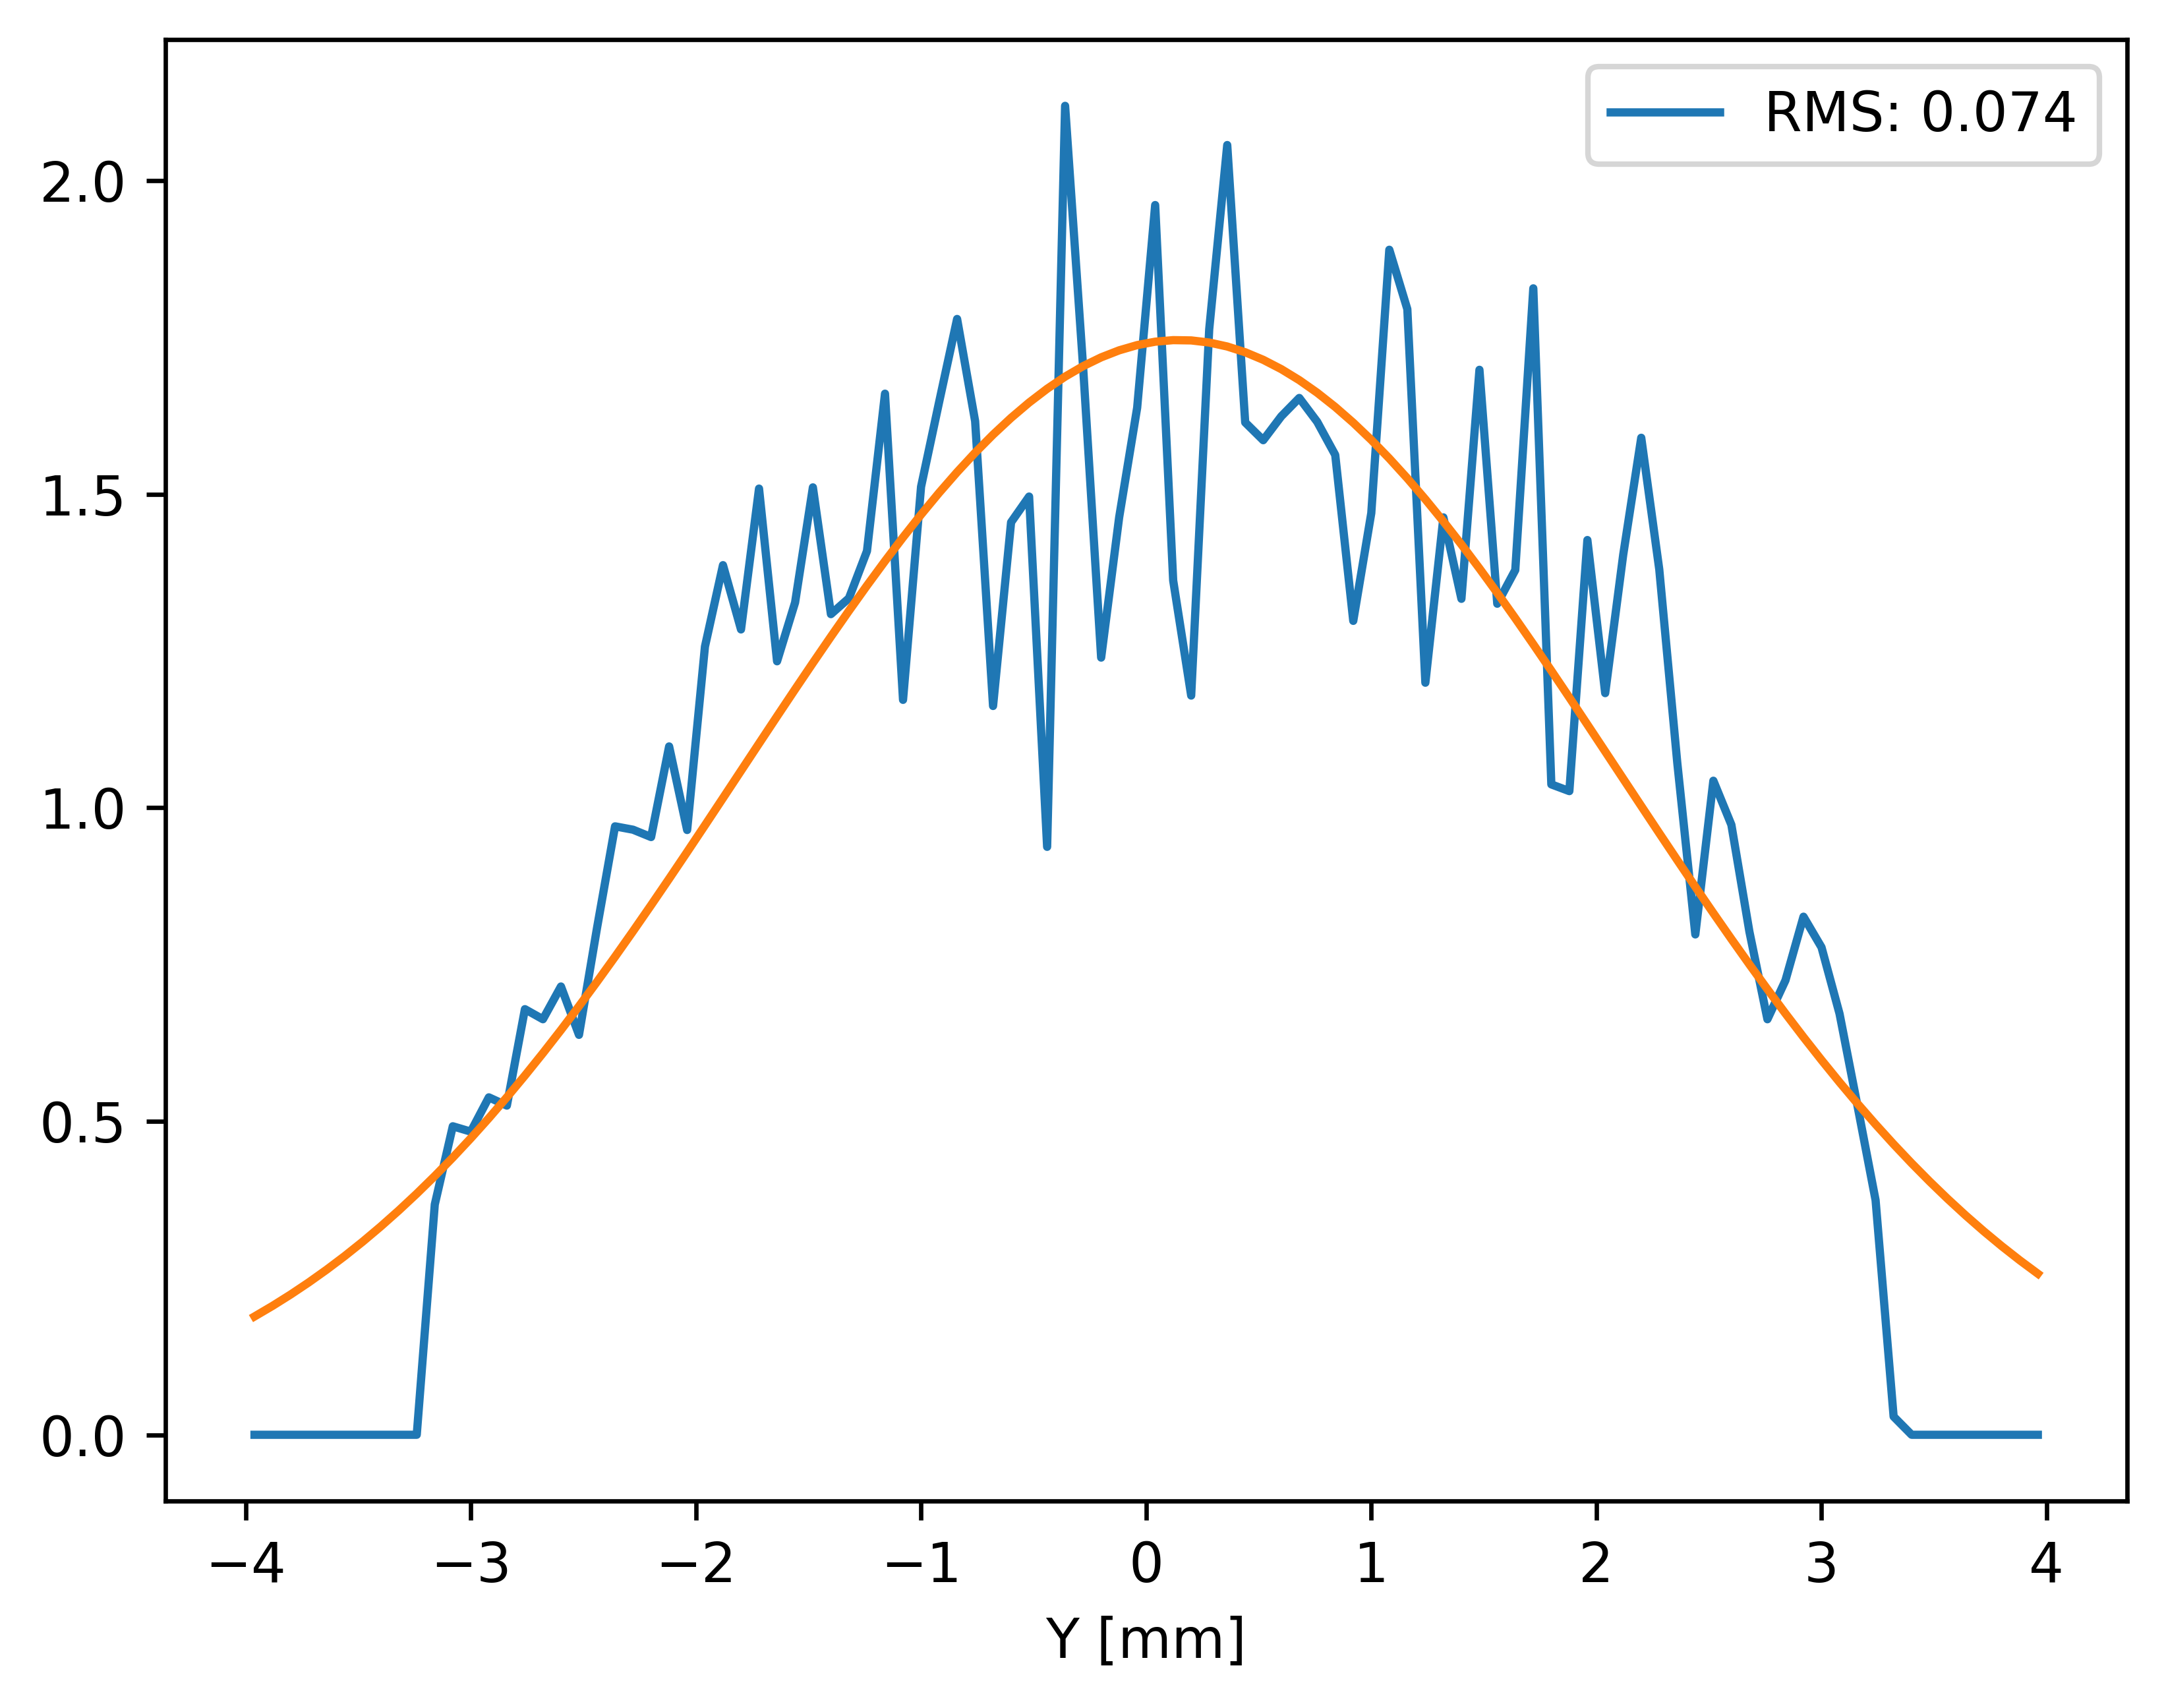
\includegraphics[width=0.9\linewidth]{./../figures/slope_error/WB4C_d30_d-spacing_gradient_45keV_slope_error025urad_Yprofile.png}
\caption{0.25 urad}
\label{fig:025urad}
\end{figure}

%%%%%%%%%%%%%%%%%%%%%%%%%%%%%%%%%%%%%%%%%%%%%%%%%%%%%%%%%%%%%%%%%%%%%%%%%%%%%%%%%%
\clearpage
\subsubsection{0.3 urad}
\begin{figure}[H]
\centering
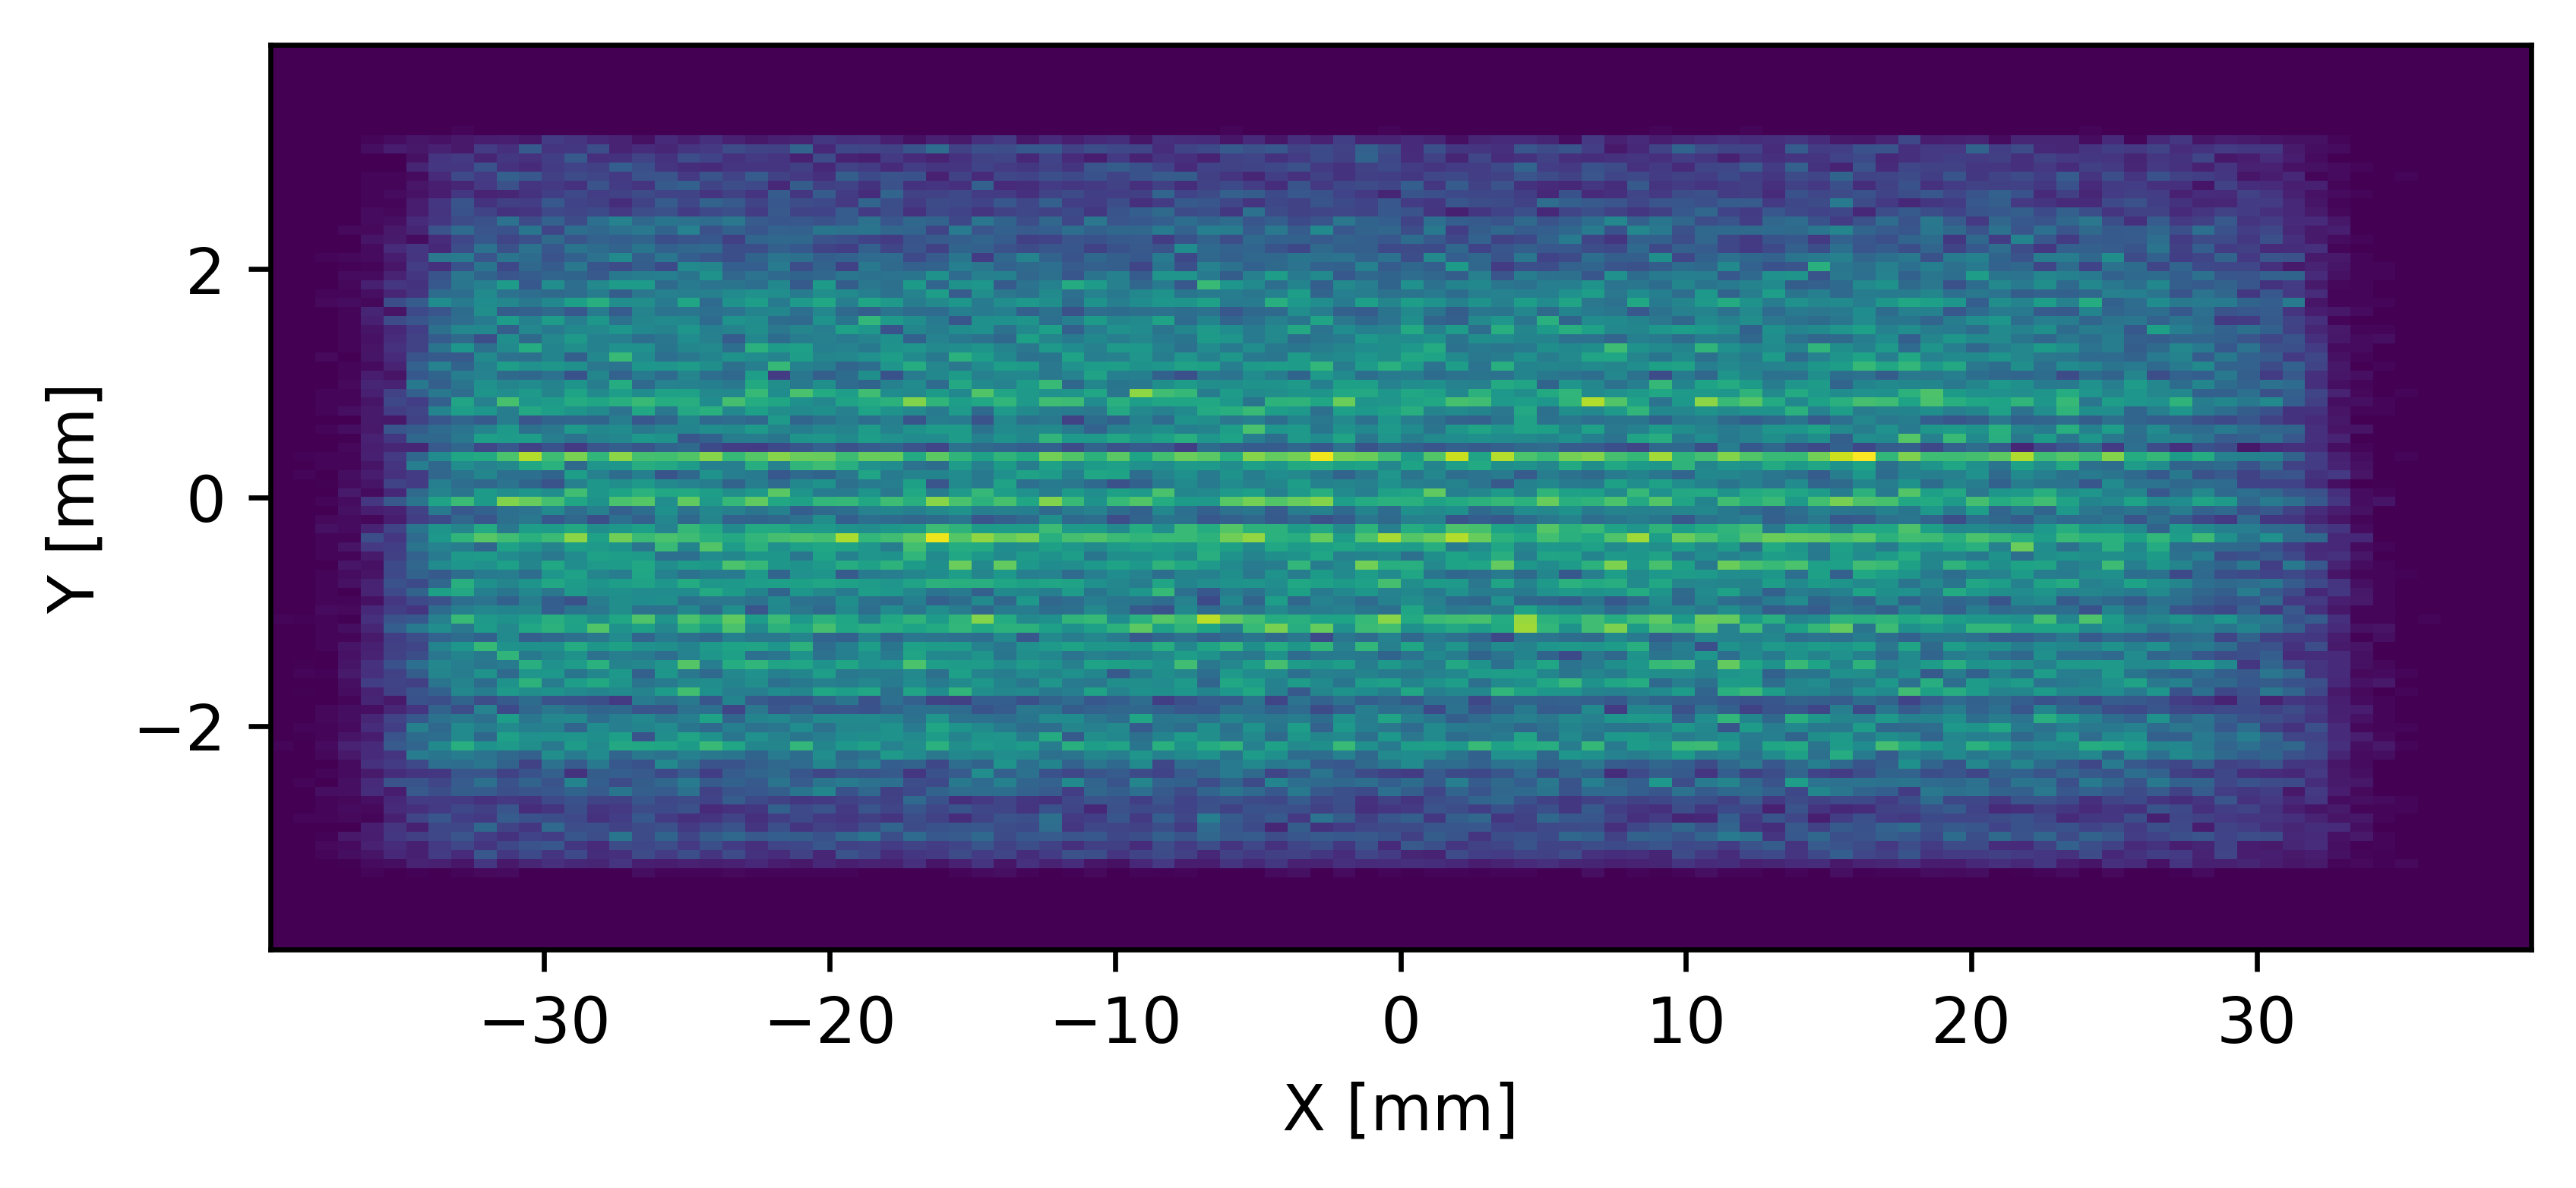
\includegraphics[width=0.9\linewidth]{./../figures/slope_error/WB4C_d30_d-spacing_gradient_45keV_slope_error03urad.png}
\end{figure}

\begin{figure}[H]
\centering
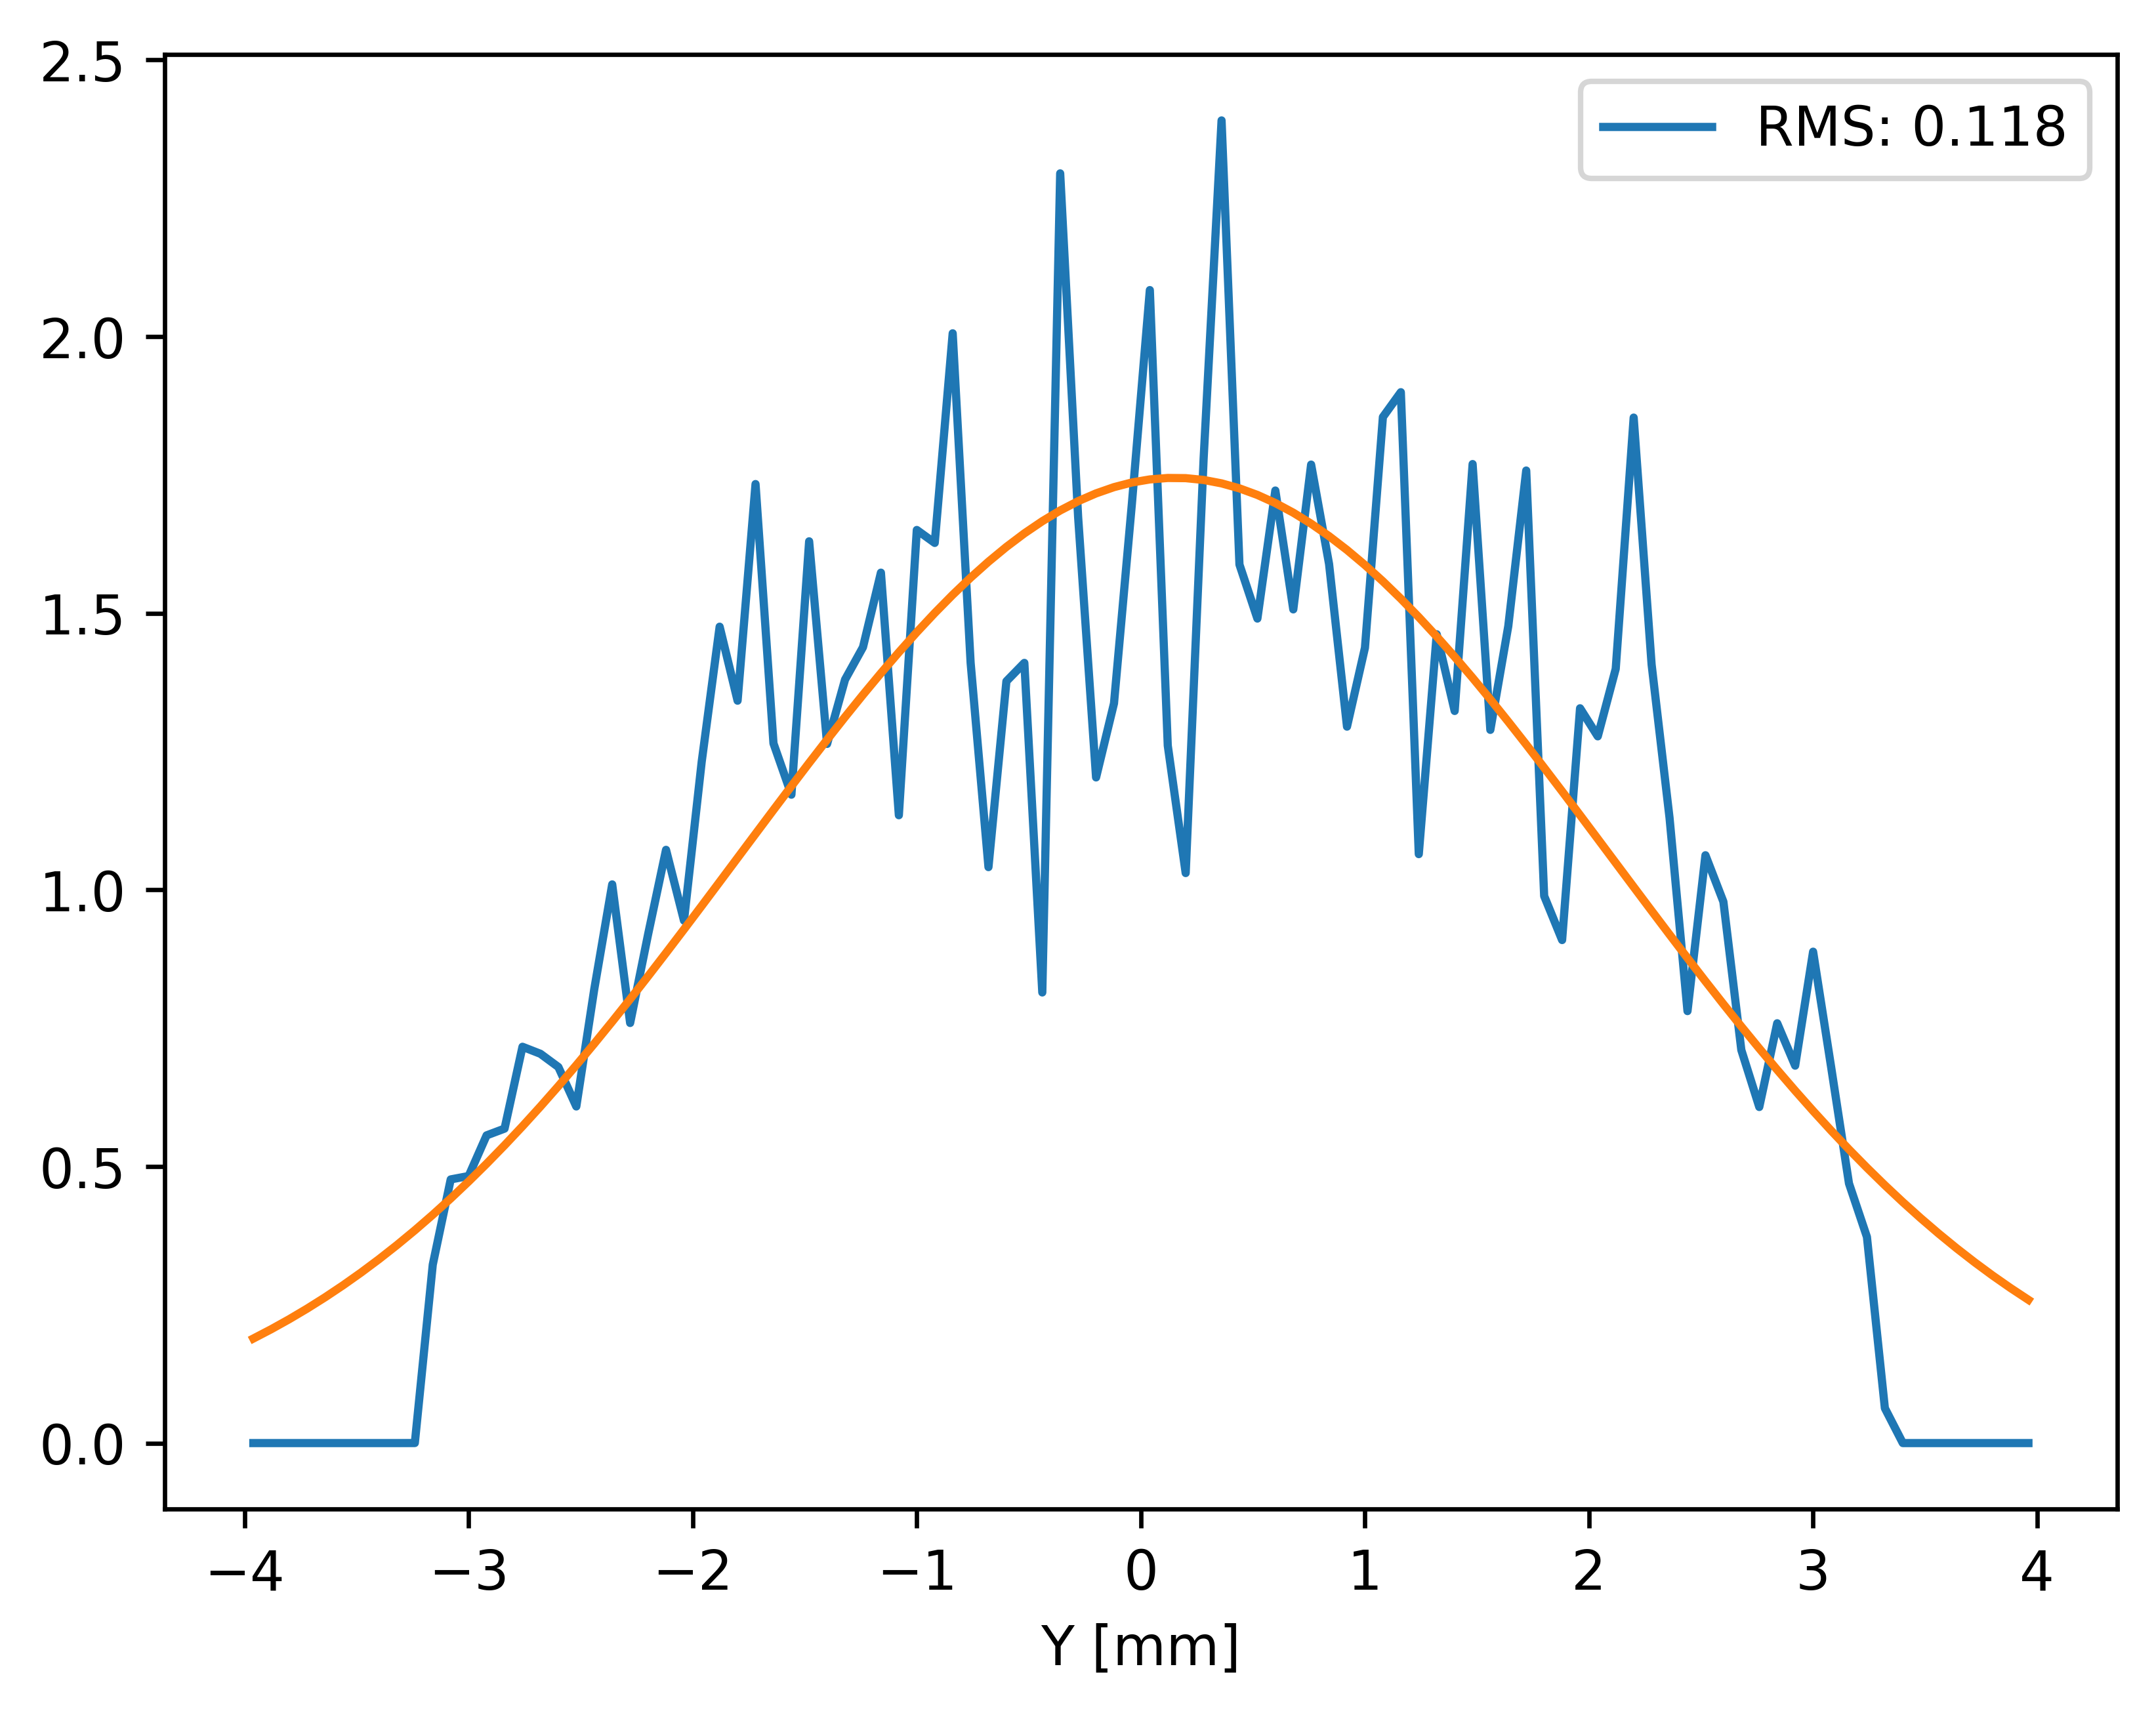
\includegraphics[width=0.9\linewidth]{./../figures/slope_error/WB4C_d30_d-spacing_gradient_45keV_slope_error03urad_Yprofile.png}
\caption{0.3 urad}
\label{fig:03urad}
\end{figure}

%%%%%%%%%%%%%%%%%%%%%%%%%%%%%%%%%%%%%%%%%%%%%%%%%%%%%%%%%%%%%%%%%%%%%%%%%%%%%%%%%%
\clearpage
\subsubsection{0.35 urad}
\begin{figure}[H]
\centering
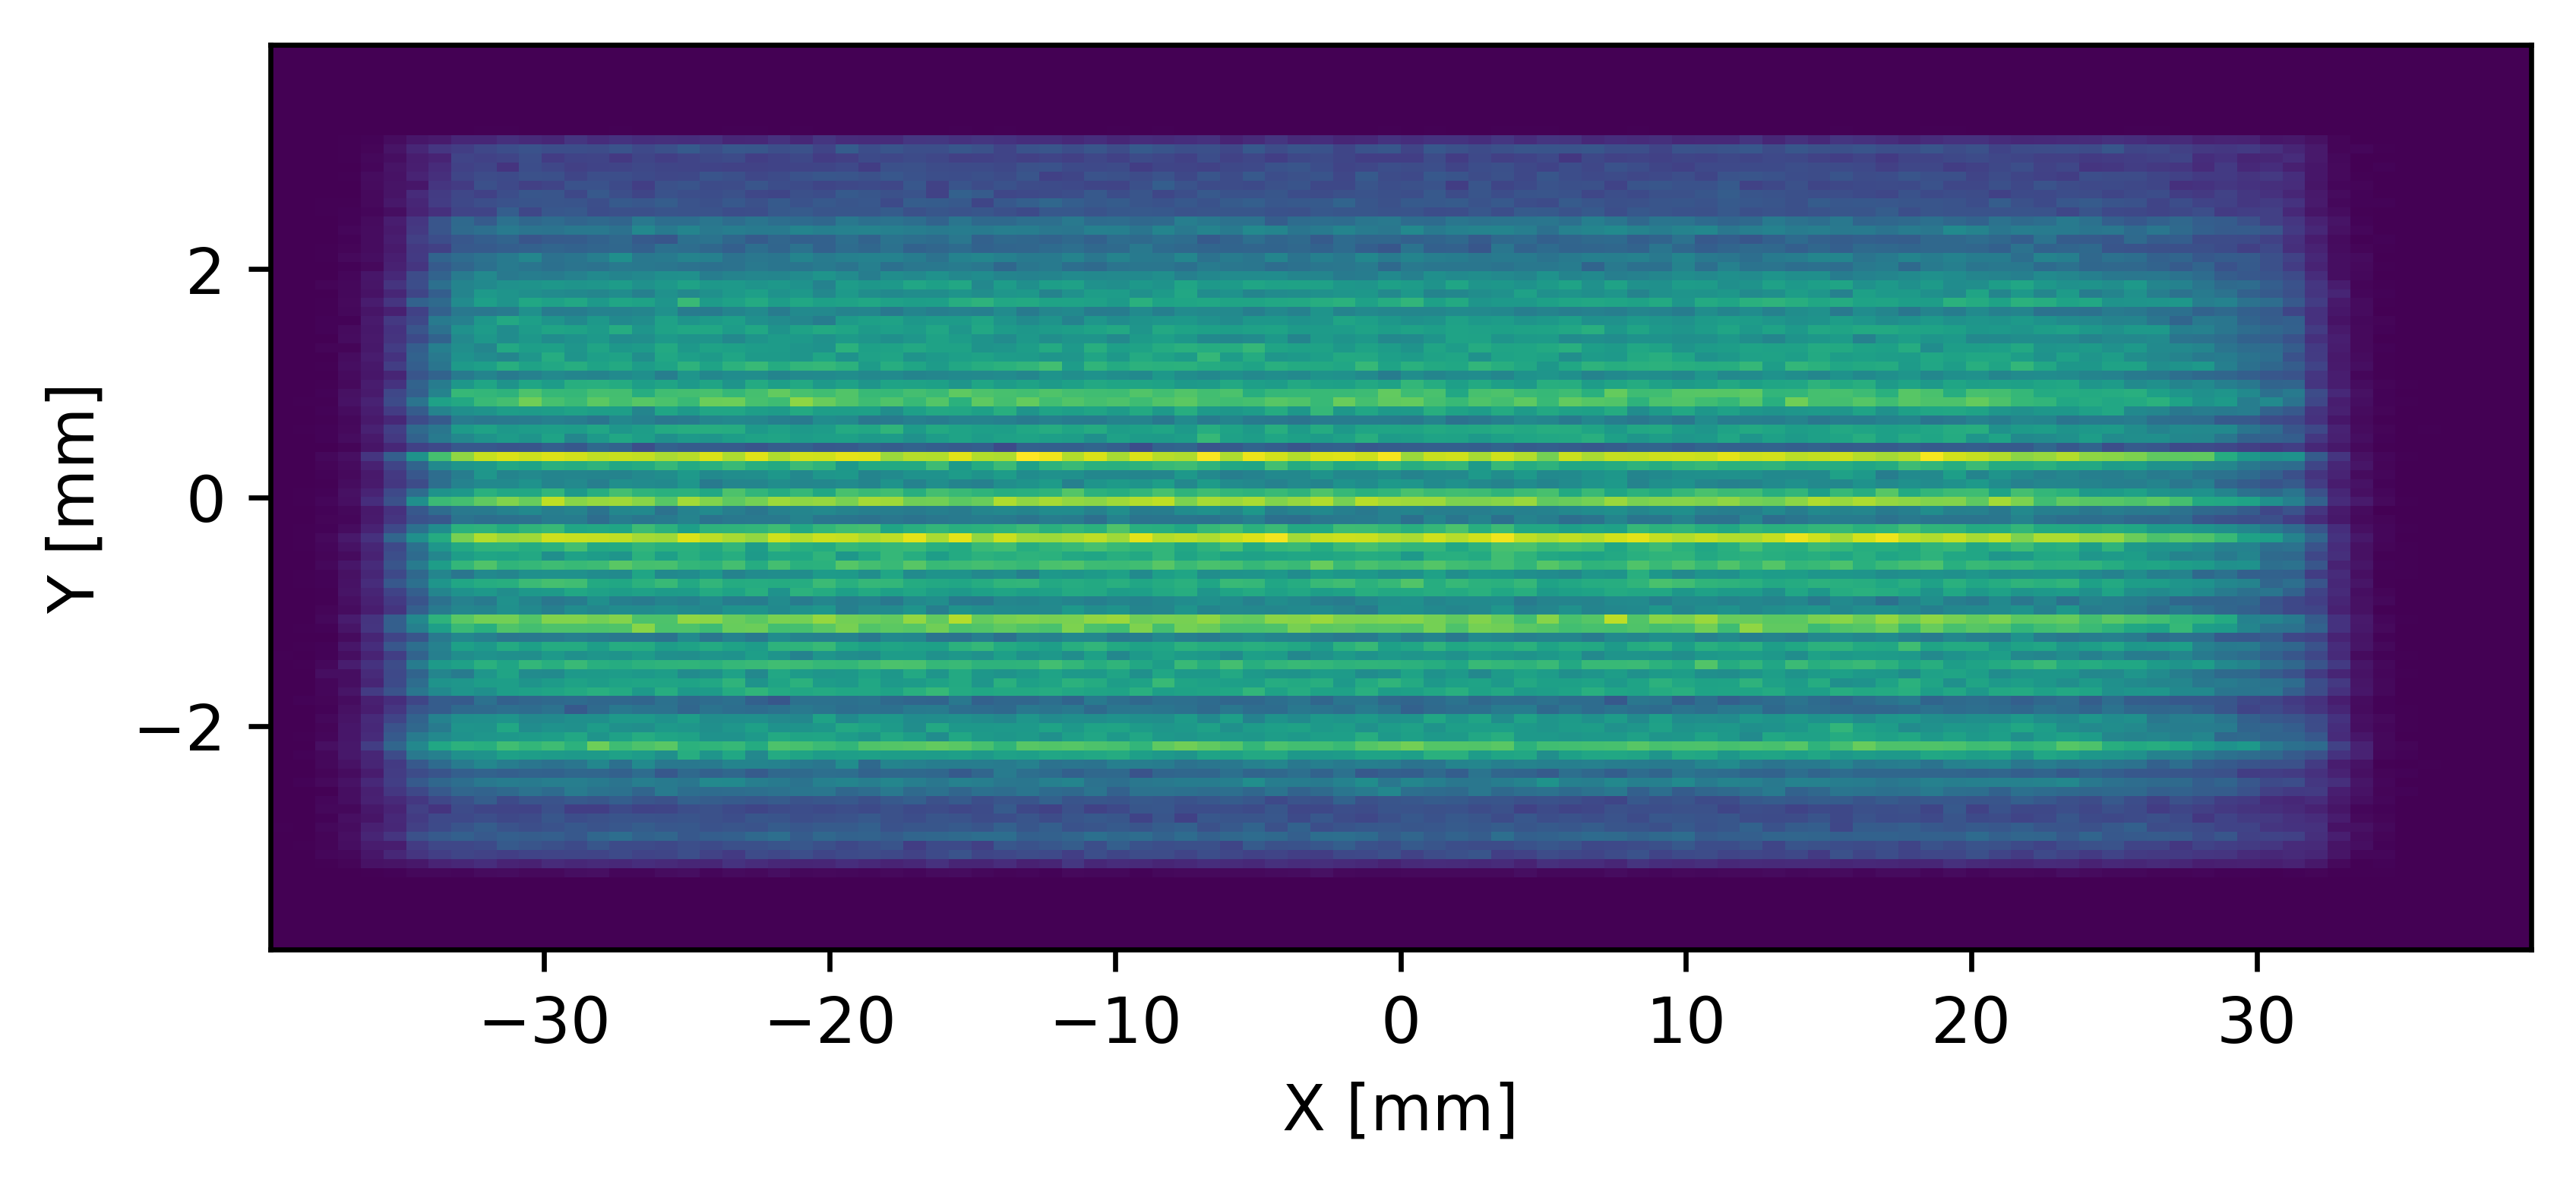
\includegraphics[width=0.9\linewidth]{./../figures/slope_error/WB4C_d30_d-spacing_gradient_45keV_slope_error035urad.png}
\end{figure}

\begin{figure}[H]
\centering
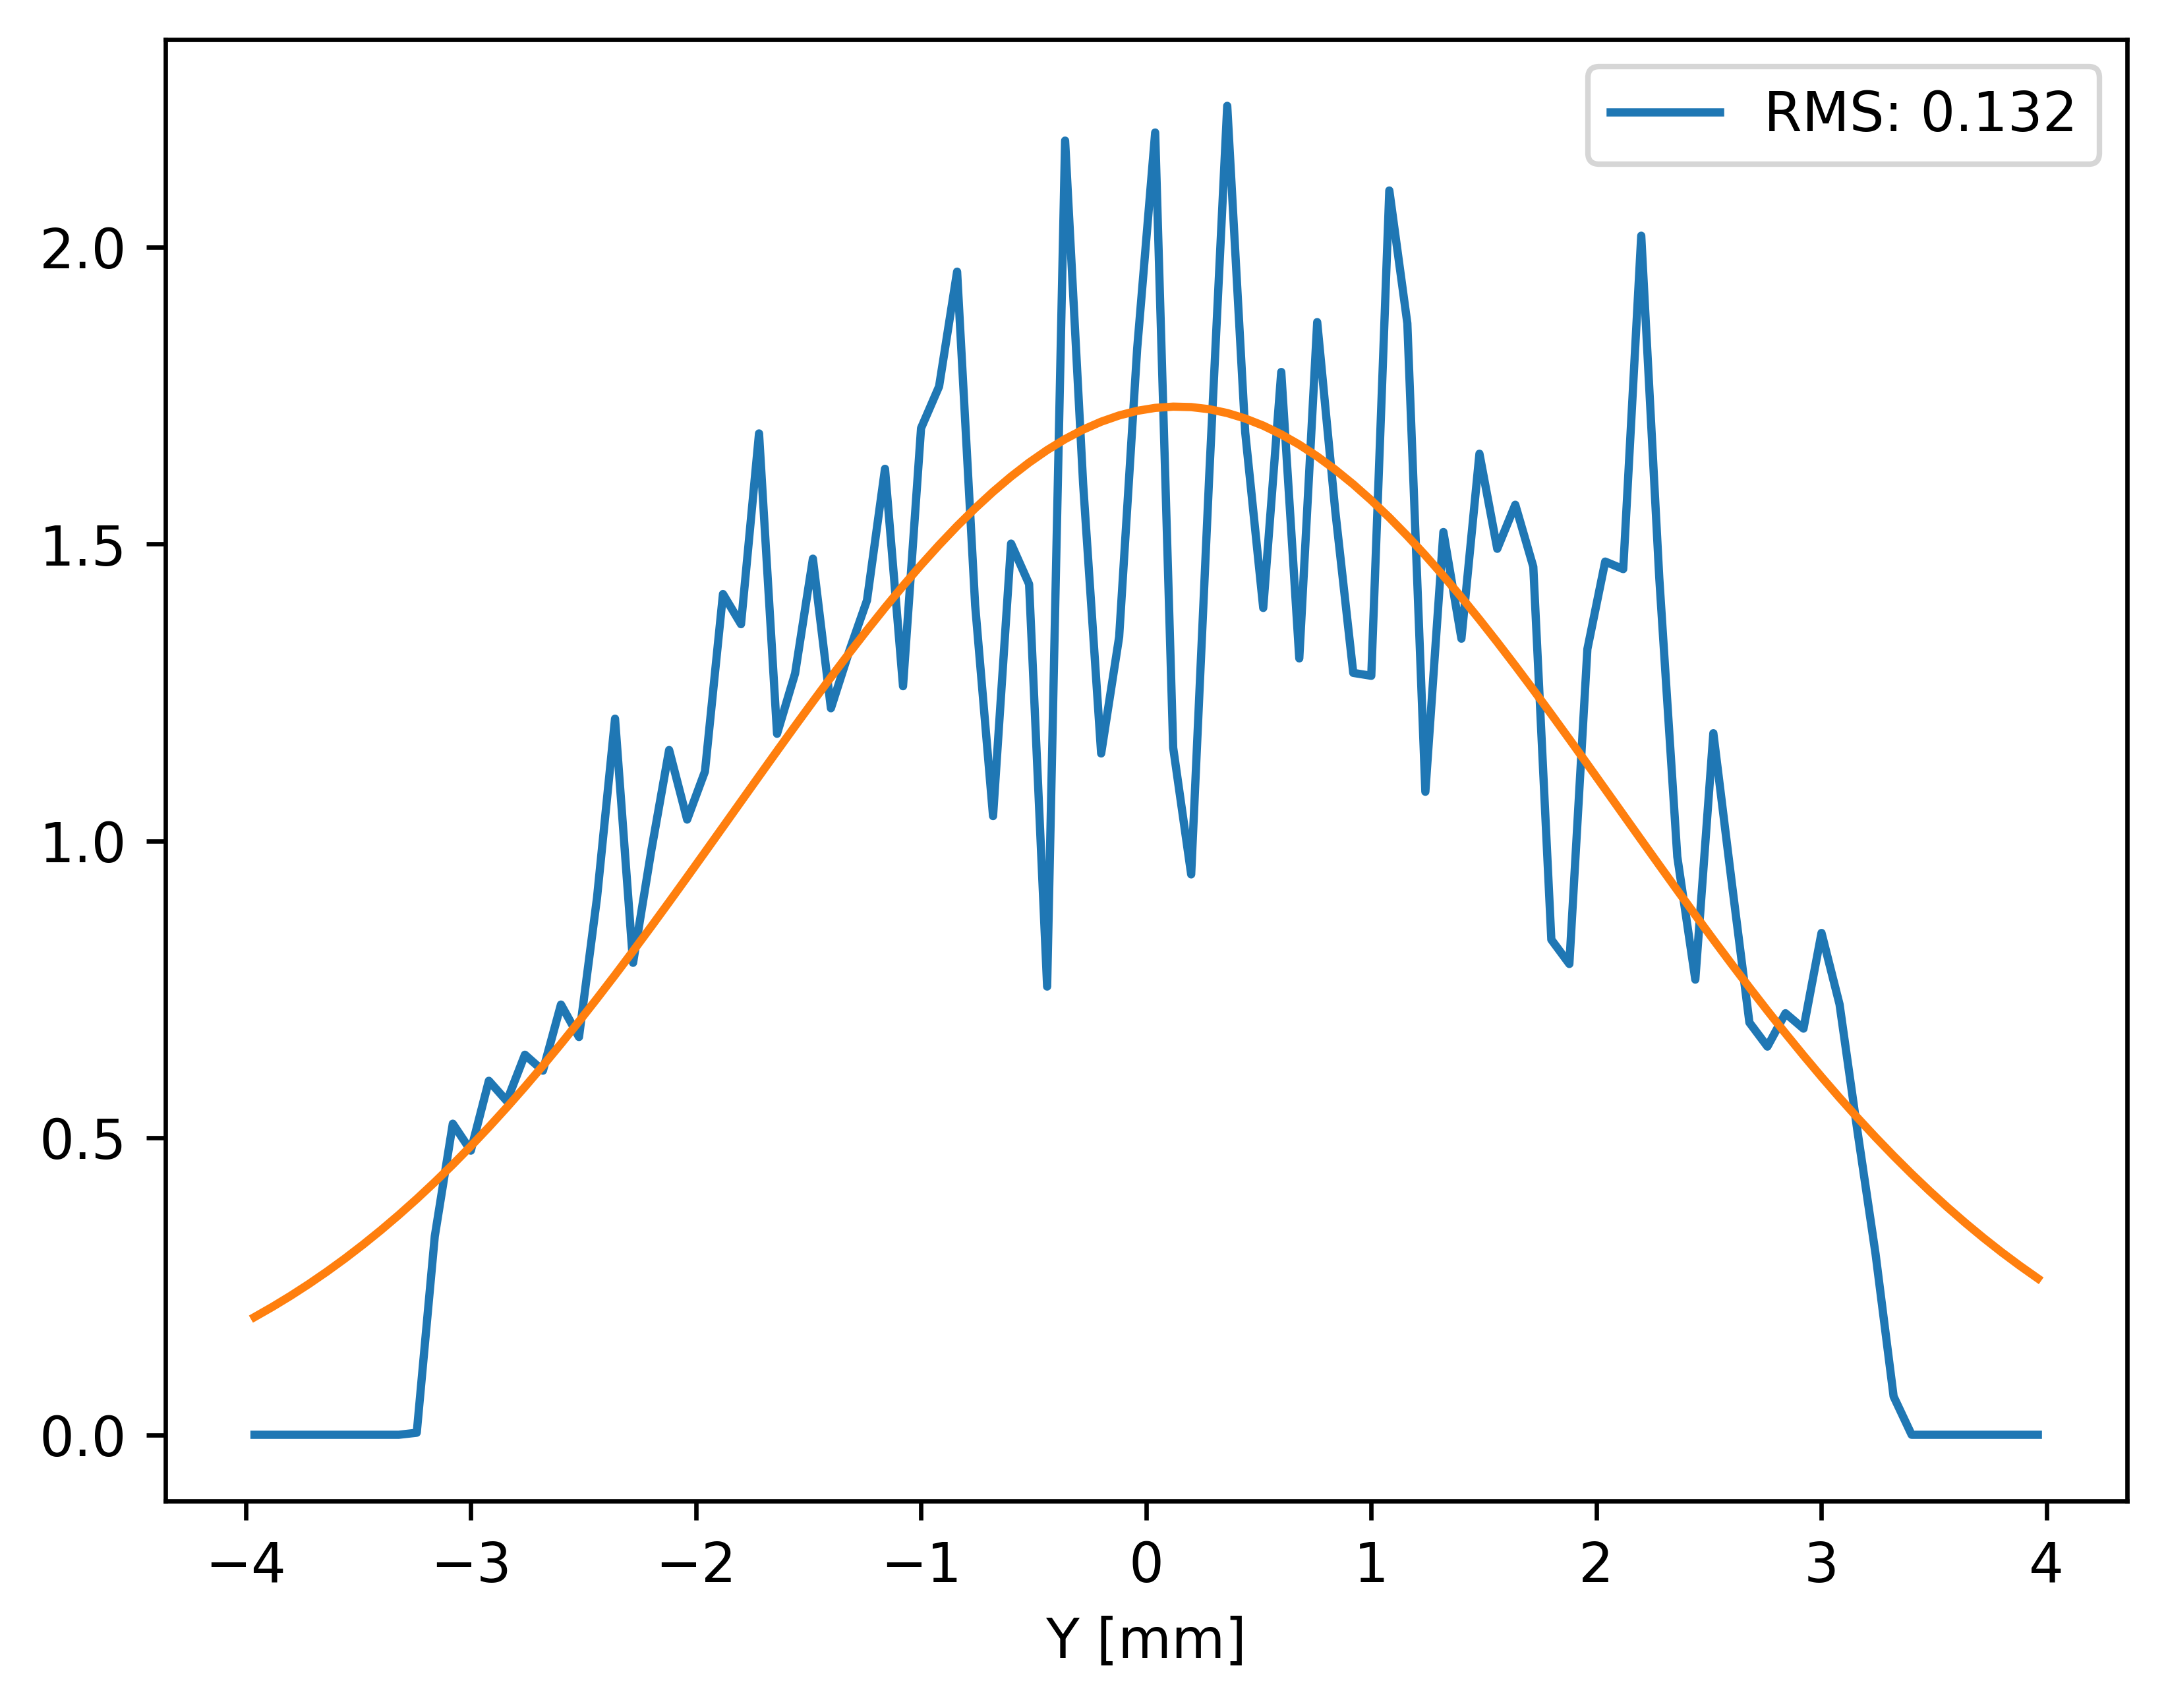
\includegraphics[width=0.9\linewidth]{./../figures/slope_error/WB4C_d30_d-spacing_gradient_45keV_slope_error035urad_Yprofile.png}
\caption{0.35 urad}
\label{fig:035urad}
\end{figure}

%%%%%%%%%%%%%%%%%%%%%%%%%%%%%%%%%%%%%%%%%%%%%%%%%%%%%%%%%%%%%%%%%%%%%%%%%%%%%%%%%%
\clearpage
\subsubsection{0.4 urad}
\begin{figure}[H]
\centering
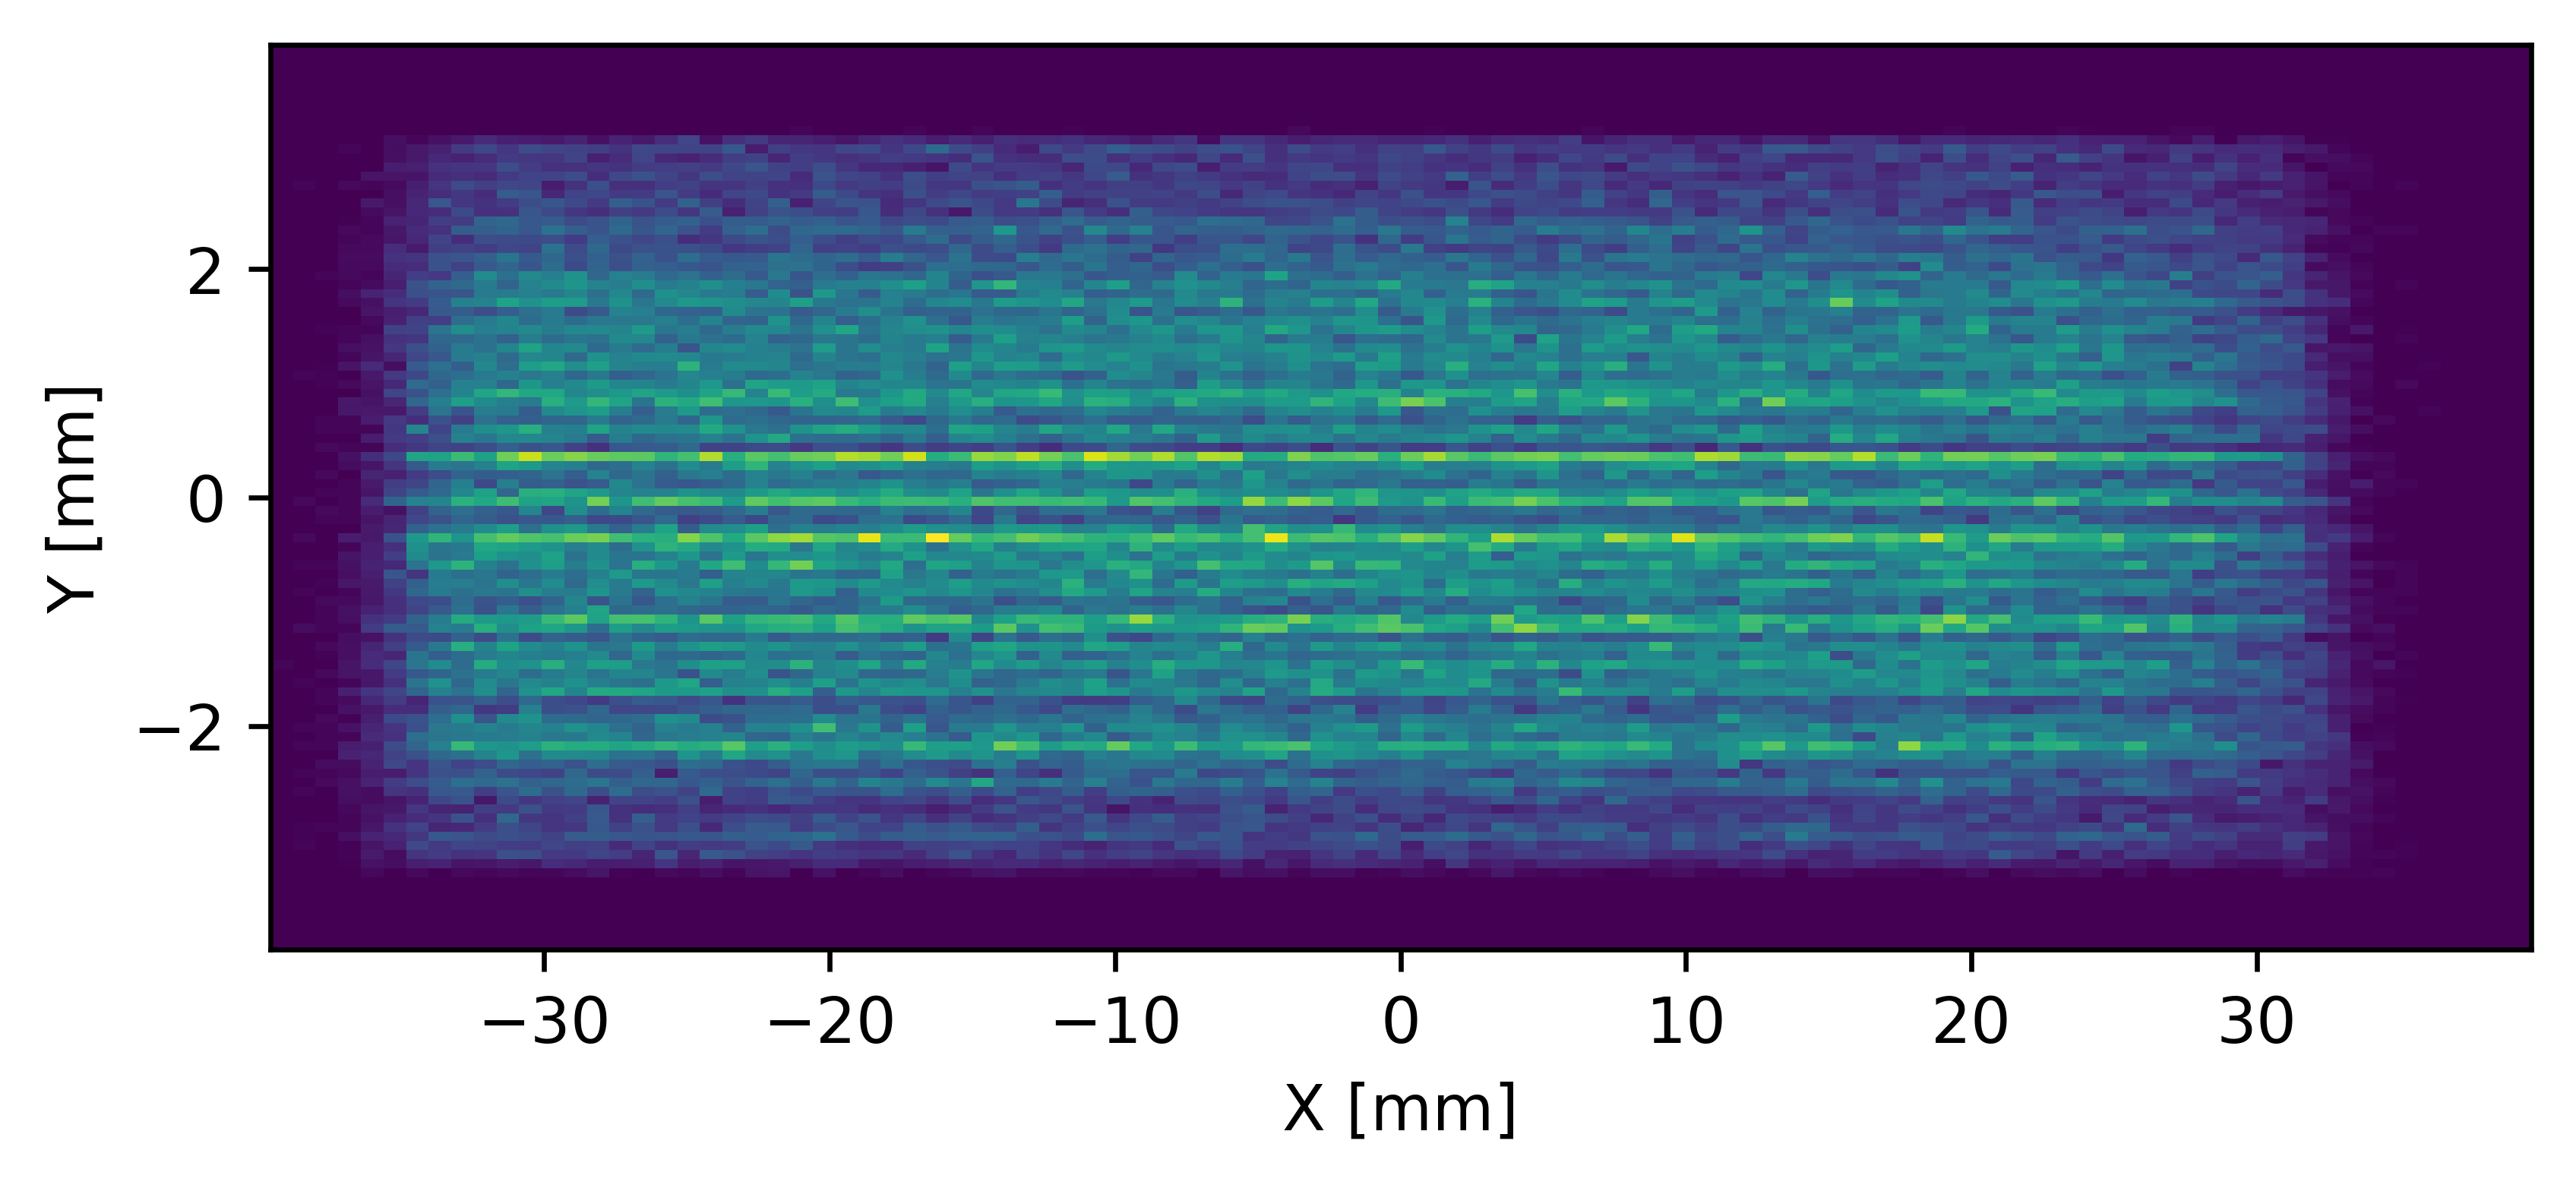
\includegraphics[width=0.9\linewidth]{./../figures/slope_error/WB4C_d30_d-spacing_gradient_45keV_slope_error04urad.png}
\end{figure}

\begin{figure}[H]
\centering
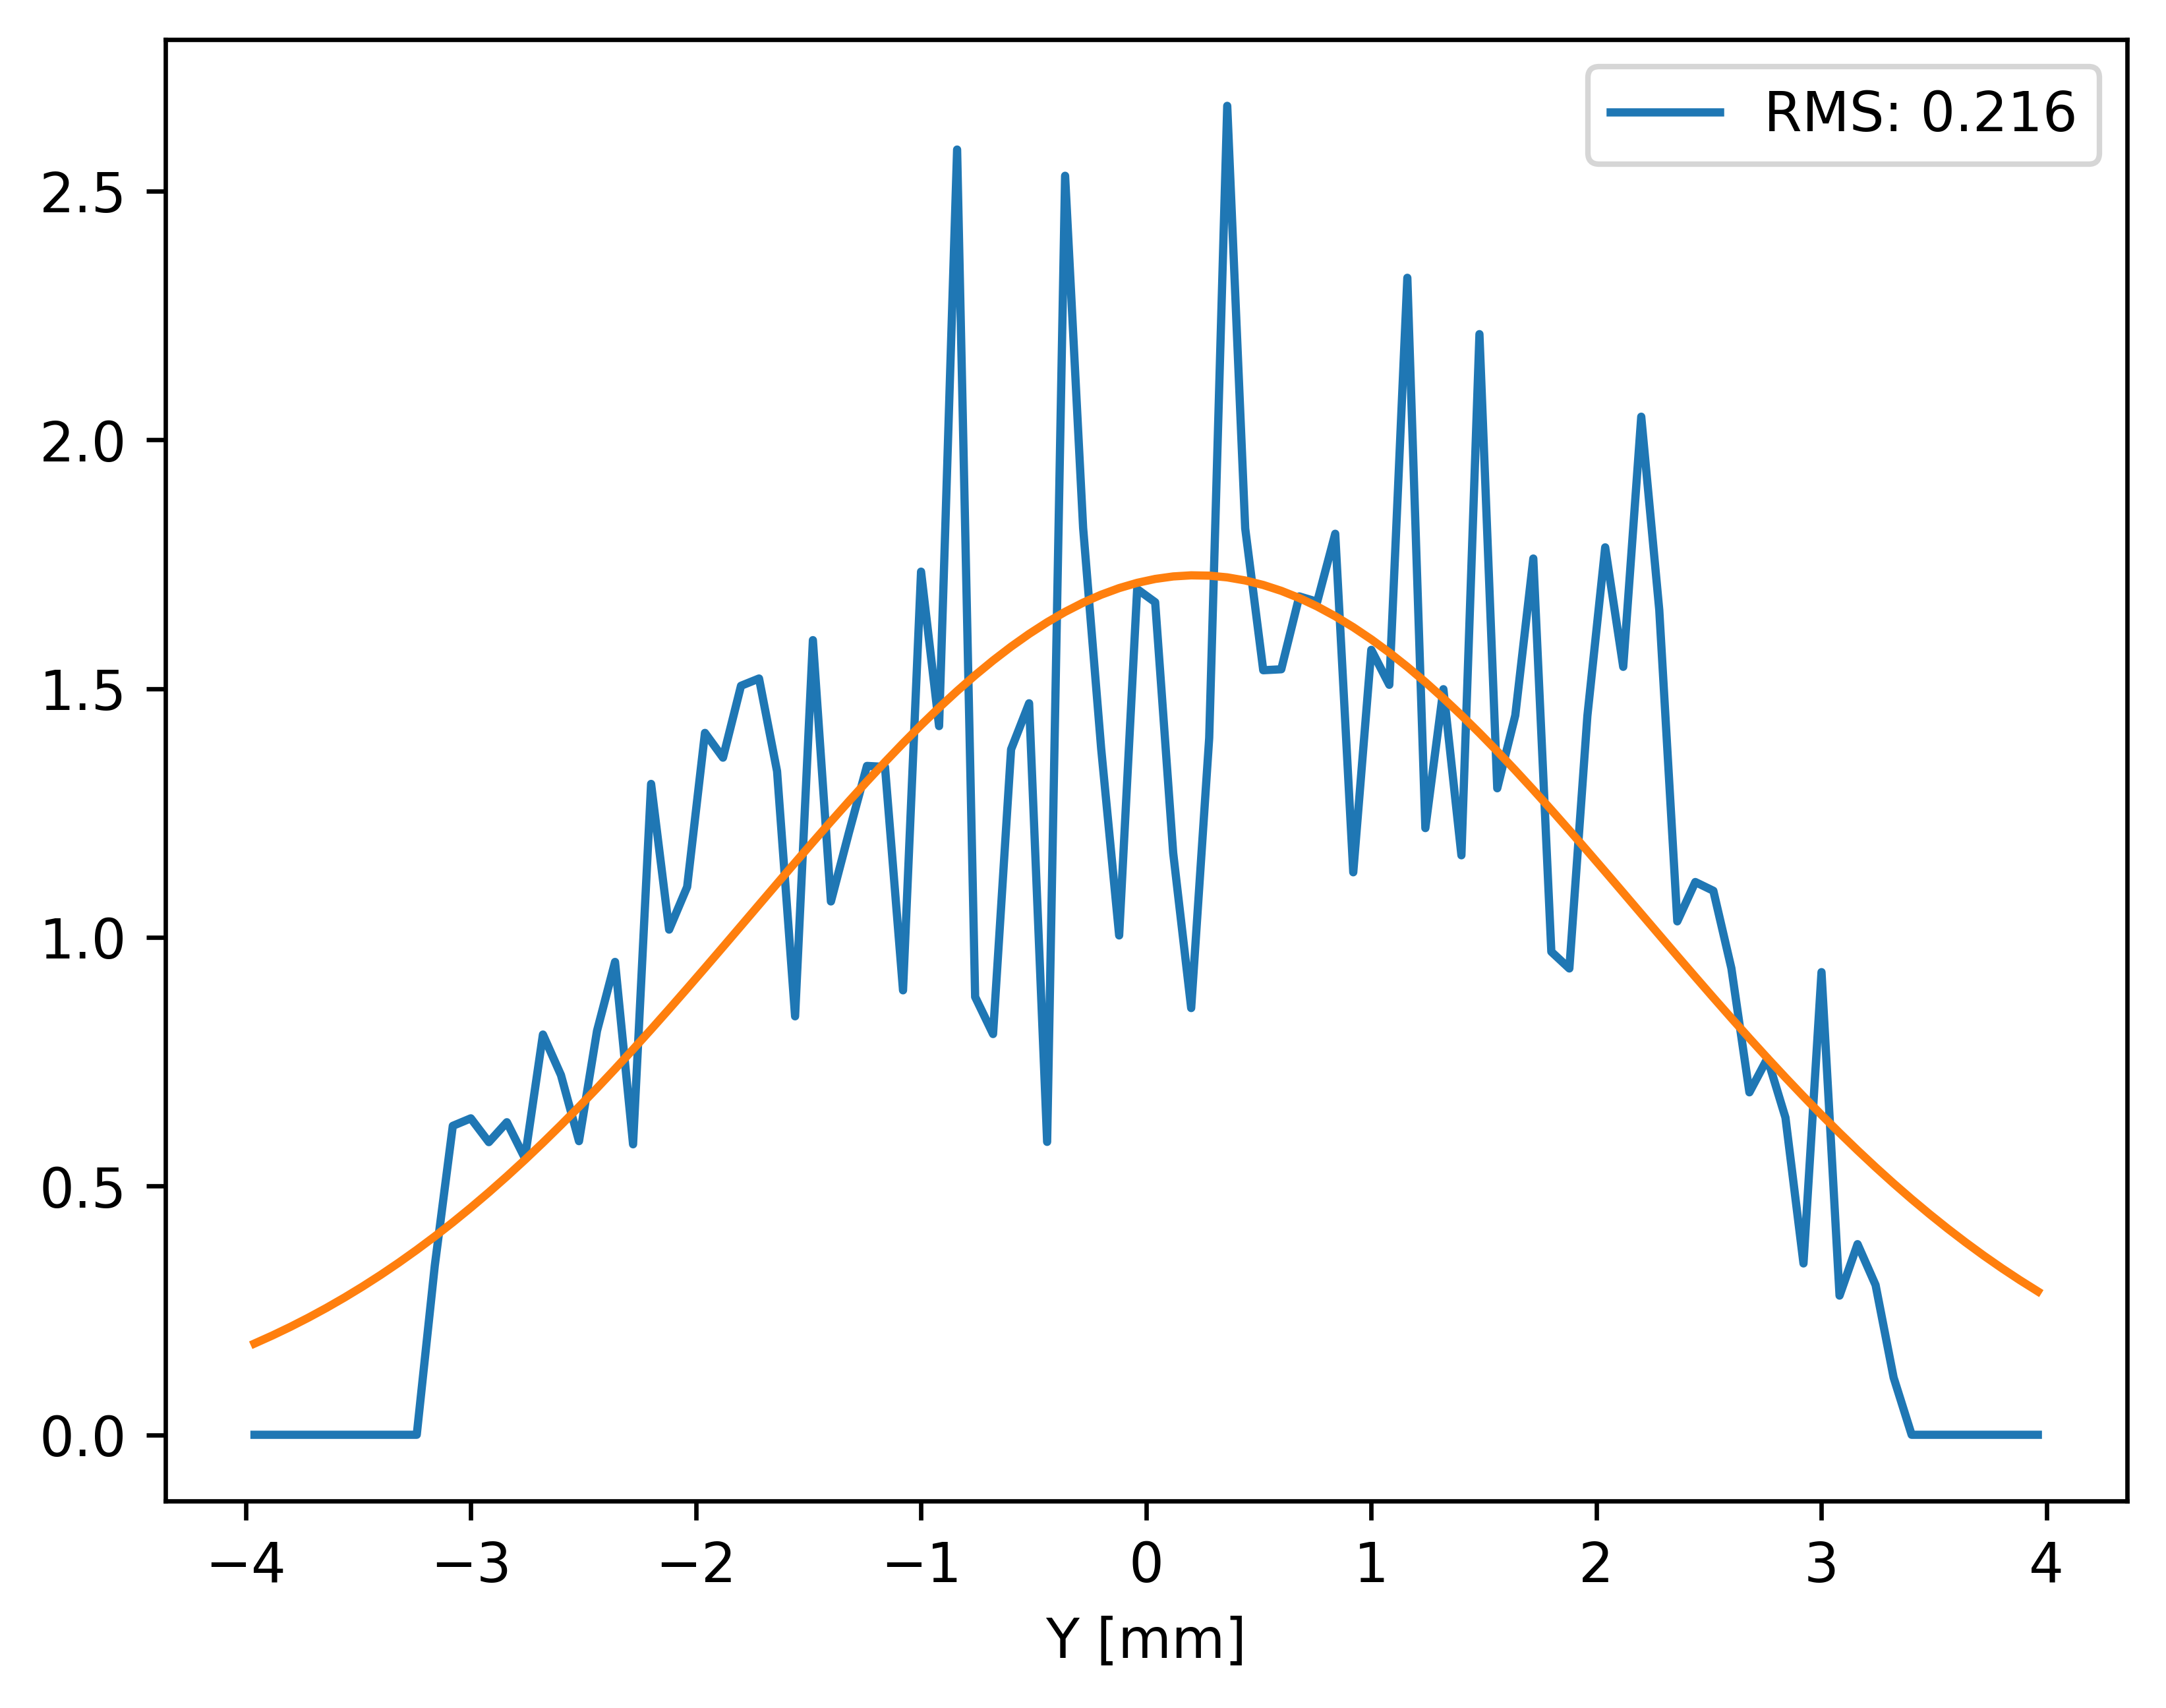
\includegraphics[width=0.9\linewidth]{./../figures/slope_error/WB4C_d30_d-spacing_gradient_45keV_slope_error04urad_Yprofile.png}
\caption{0.4 urad}
\label{fig:04urad}
\end{figure}

%%%%%%%%%%%%%%%%%%%%%%%%%%%%%%%%%%%%%%%%%%%%%%%%%%%%%%%%%%%%%%%%%%%%%%%%%%%%%%%%%%
\clearpage
\subsubsection{0.5 urad}
\begin{figure}[H]
\centering
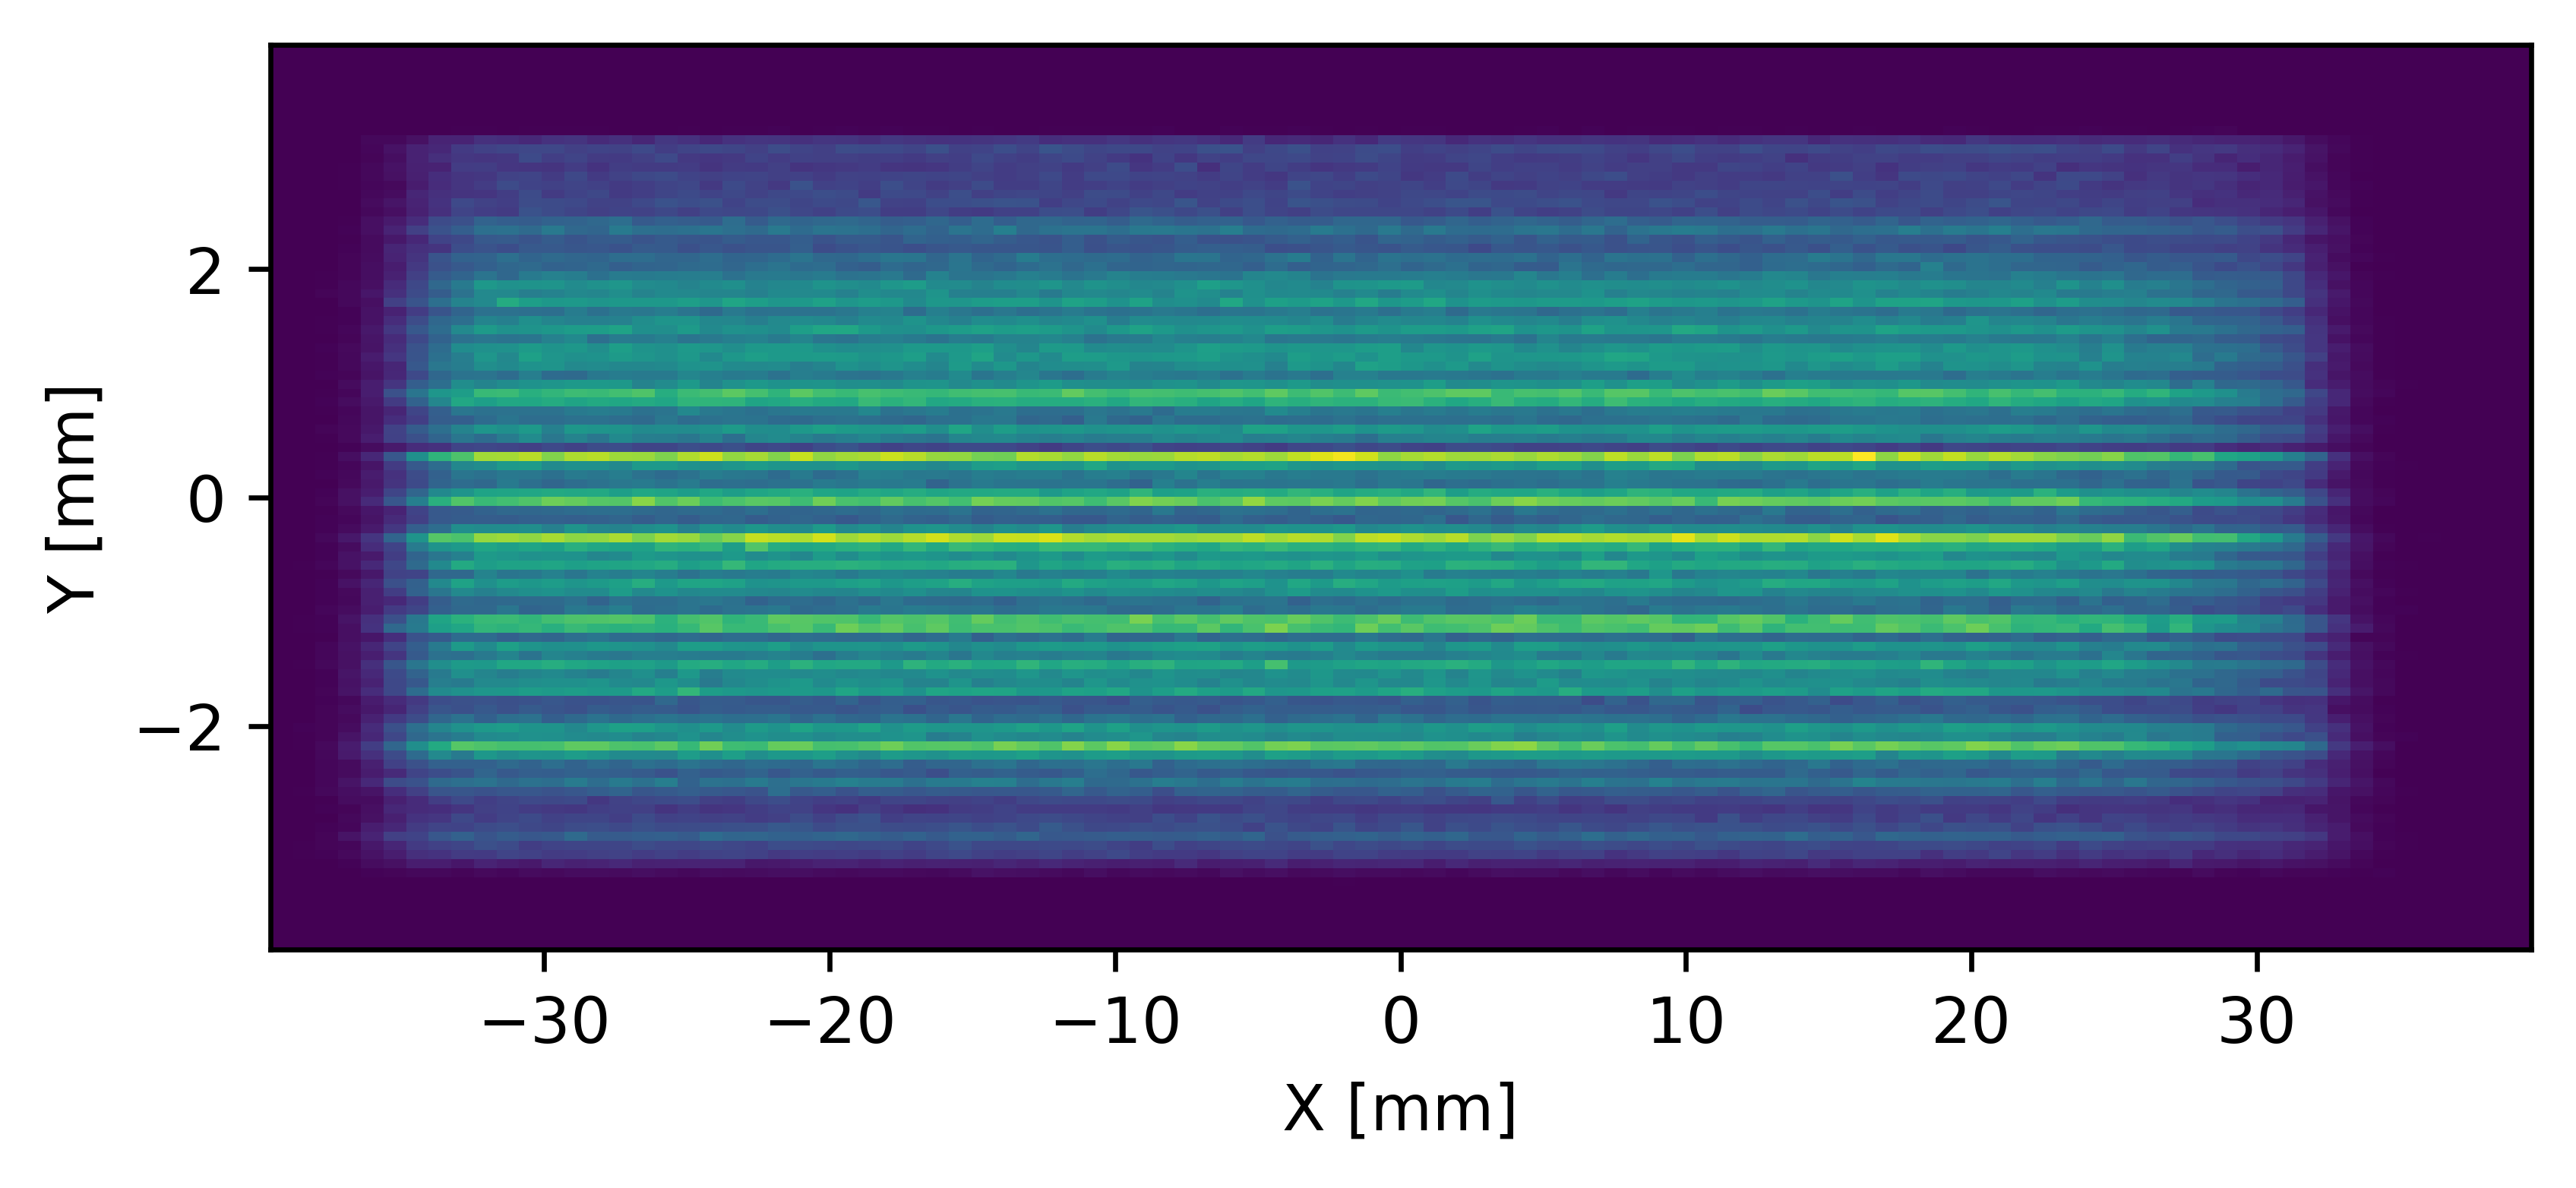
\includegraphics[width=0.9\linewidth]{./../figures/slope_error/WB4C_d30_d-spacing_gradient_45keV_slope_error05urad.png}
\end{figure}

\begin{figure}[H]
\centering
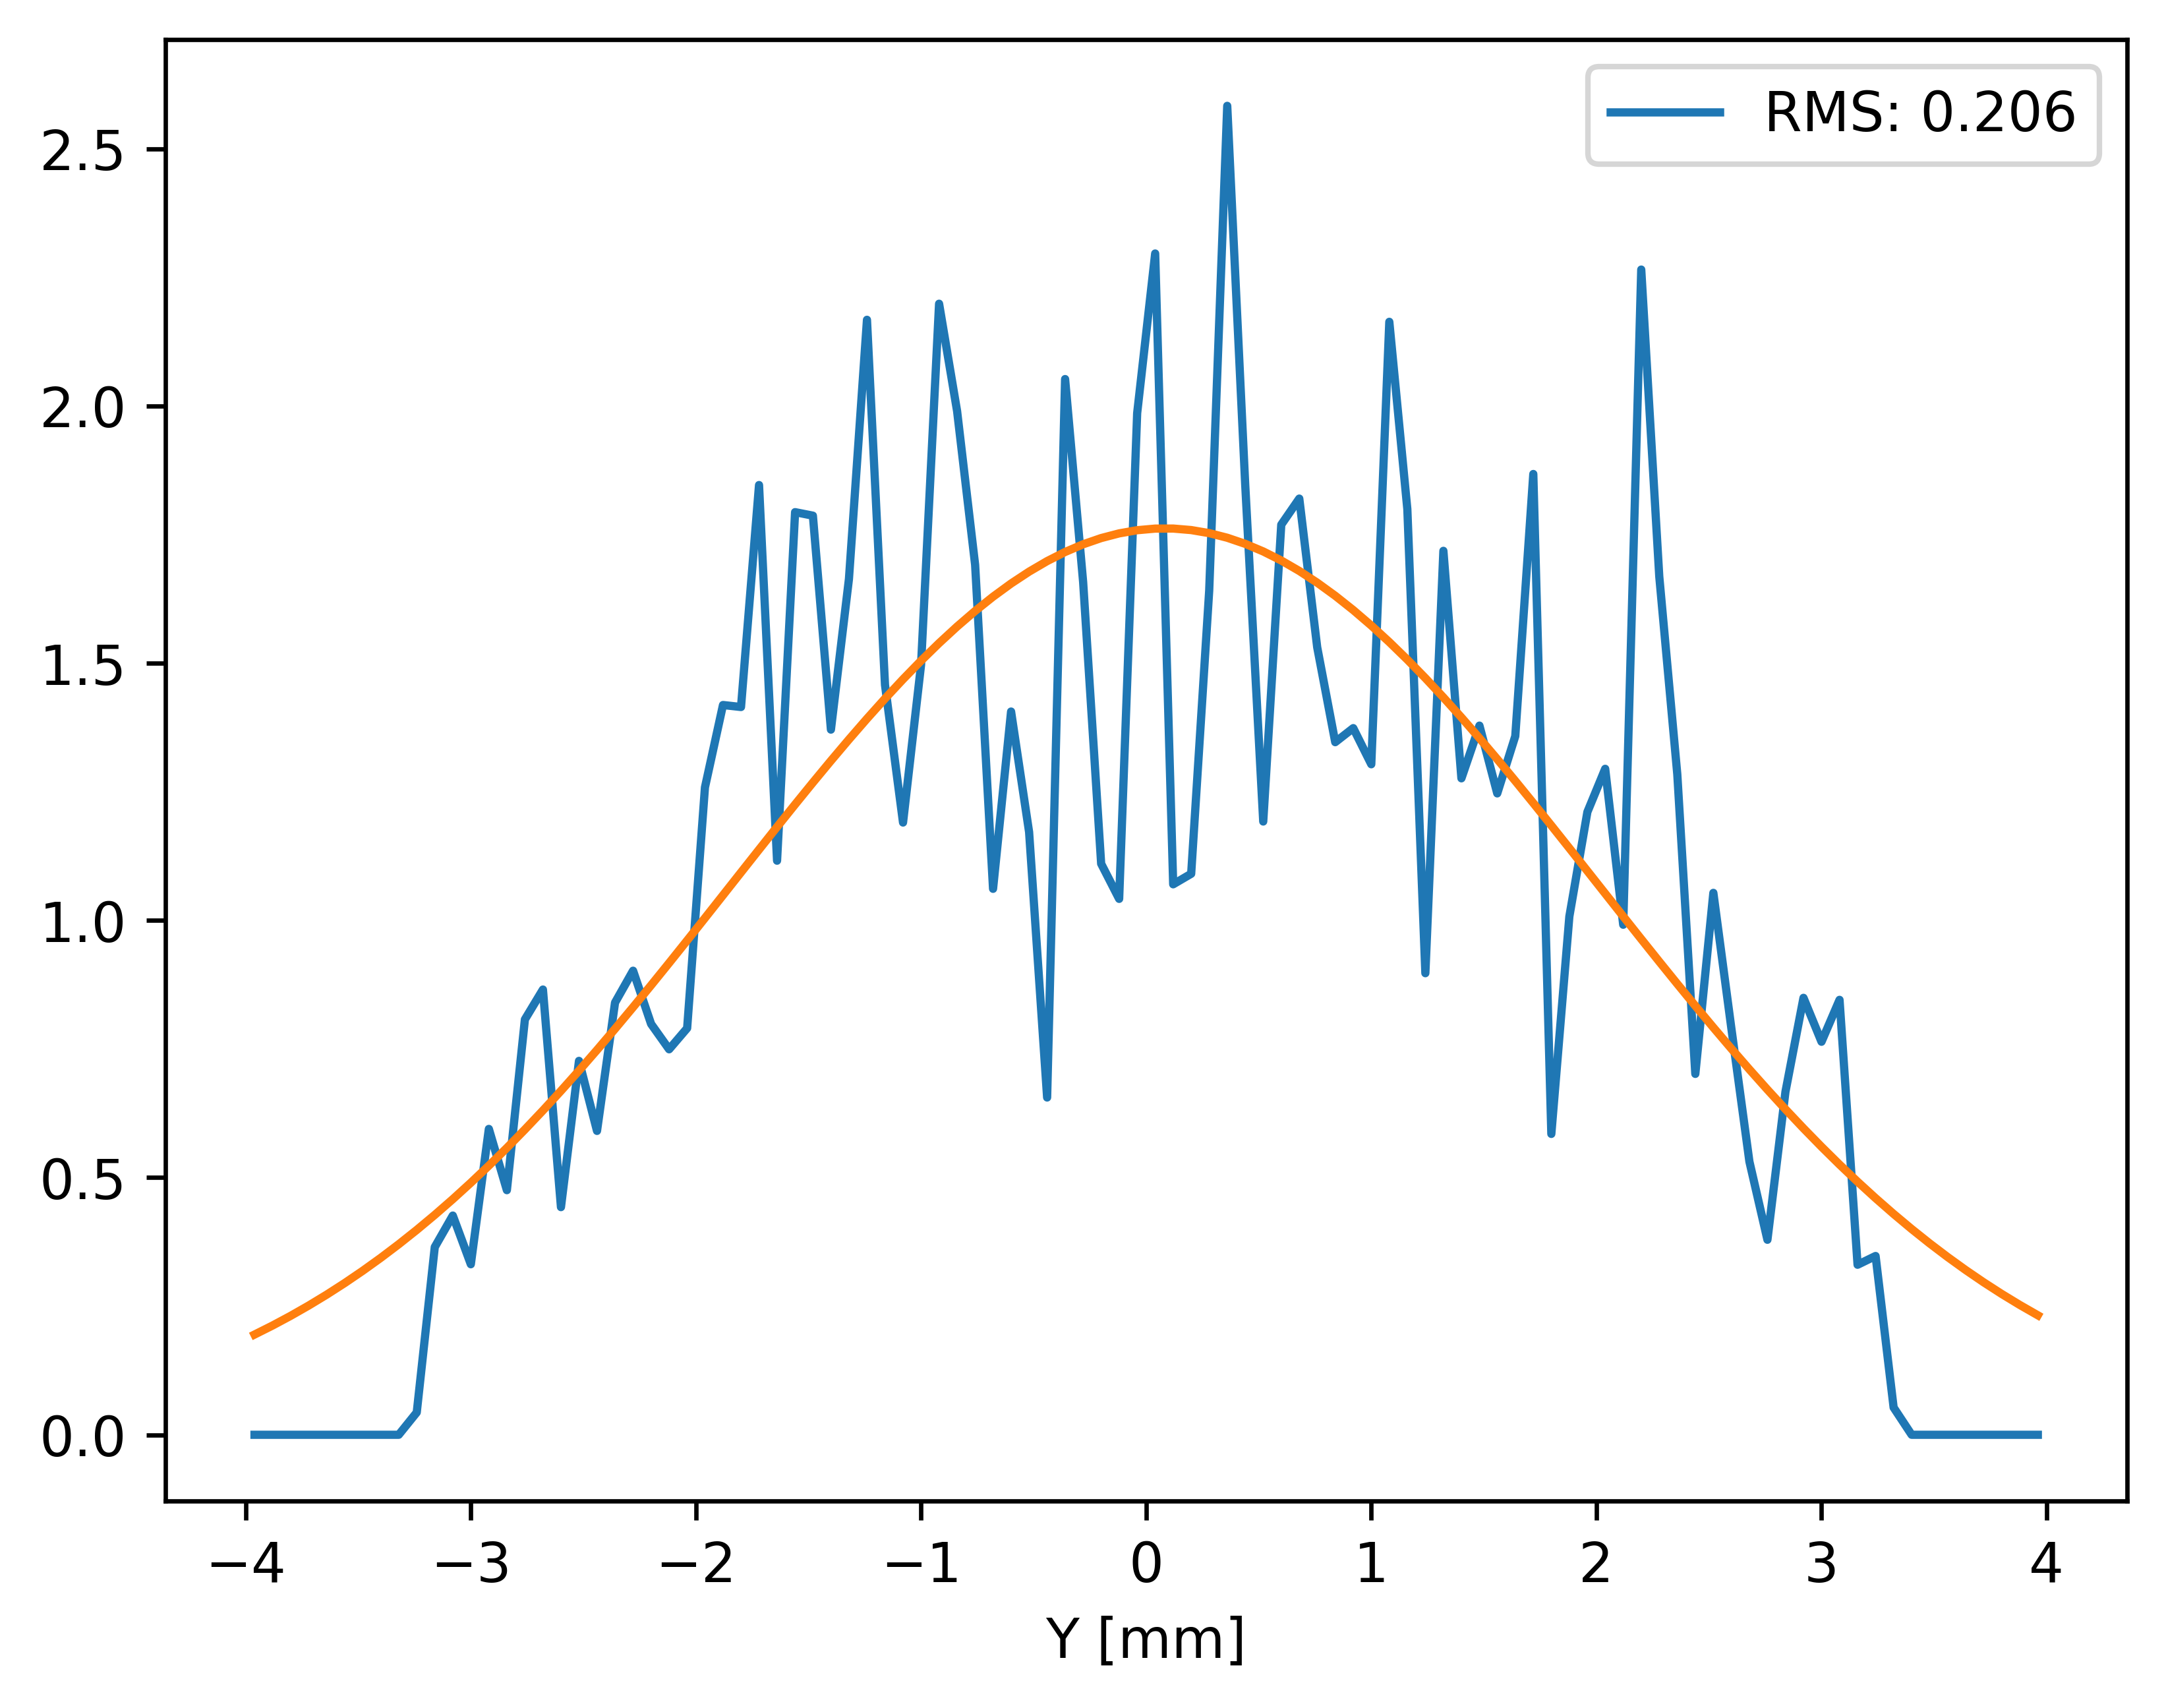
\includegraphics[width=0.9\linewidth]{./../figures/slope_error/WB4C_d30_d-spacing_gradient_45keV_slope_error05urad_Yprofile.png}
\caption{0.5 urad}
\label{fig:05urad}
\end{figure}

\clearpage
\subsection{Mirror slope error - ESRF ID19 source}
The ESRF ID19 PW150 source is considered for this paragraph for comparison. All remaining BL and mirror components are identical. 

\subsubsection{0.1 urad}
\begin{figure}[H]
\centering
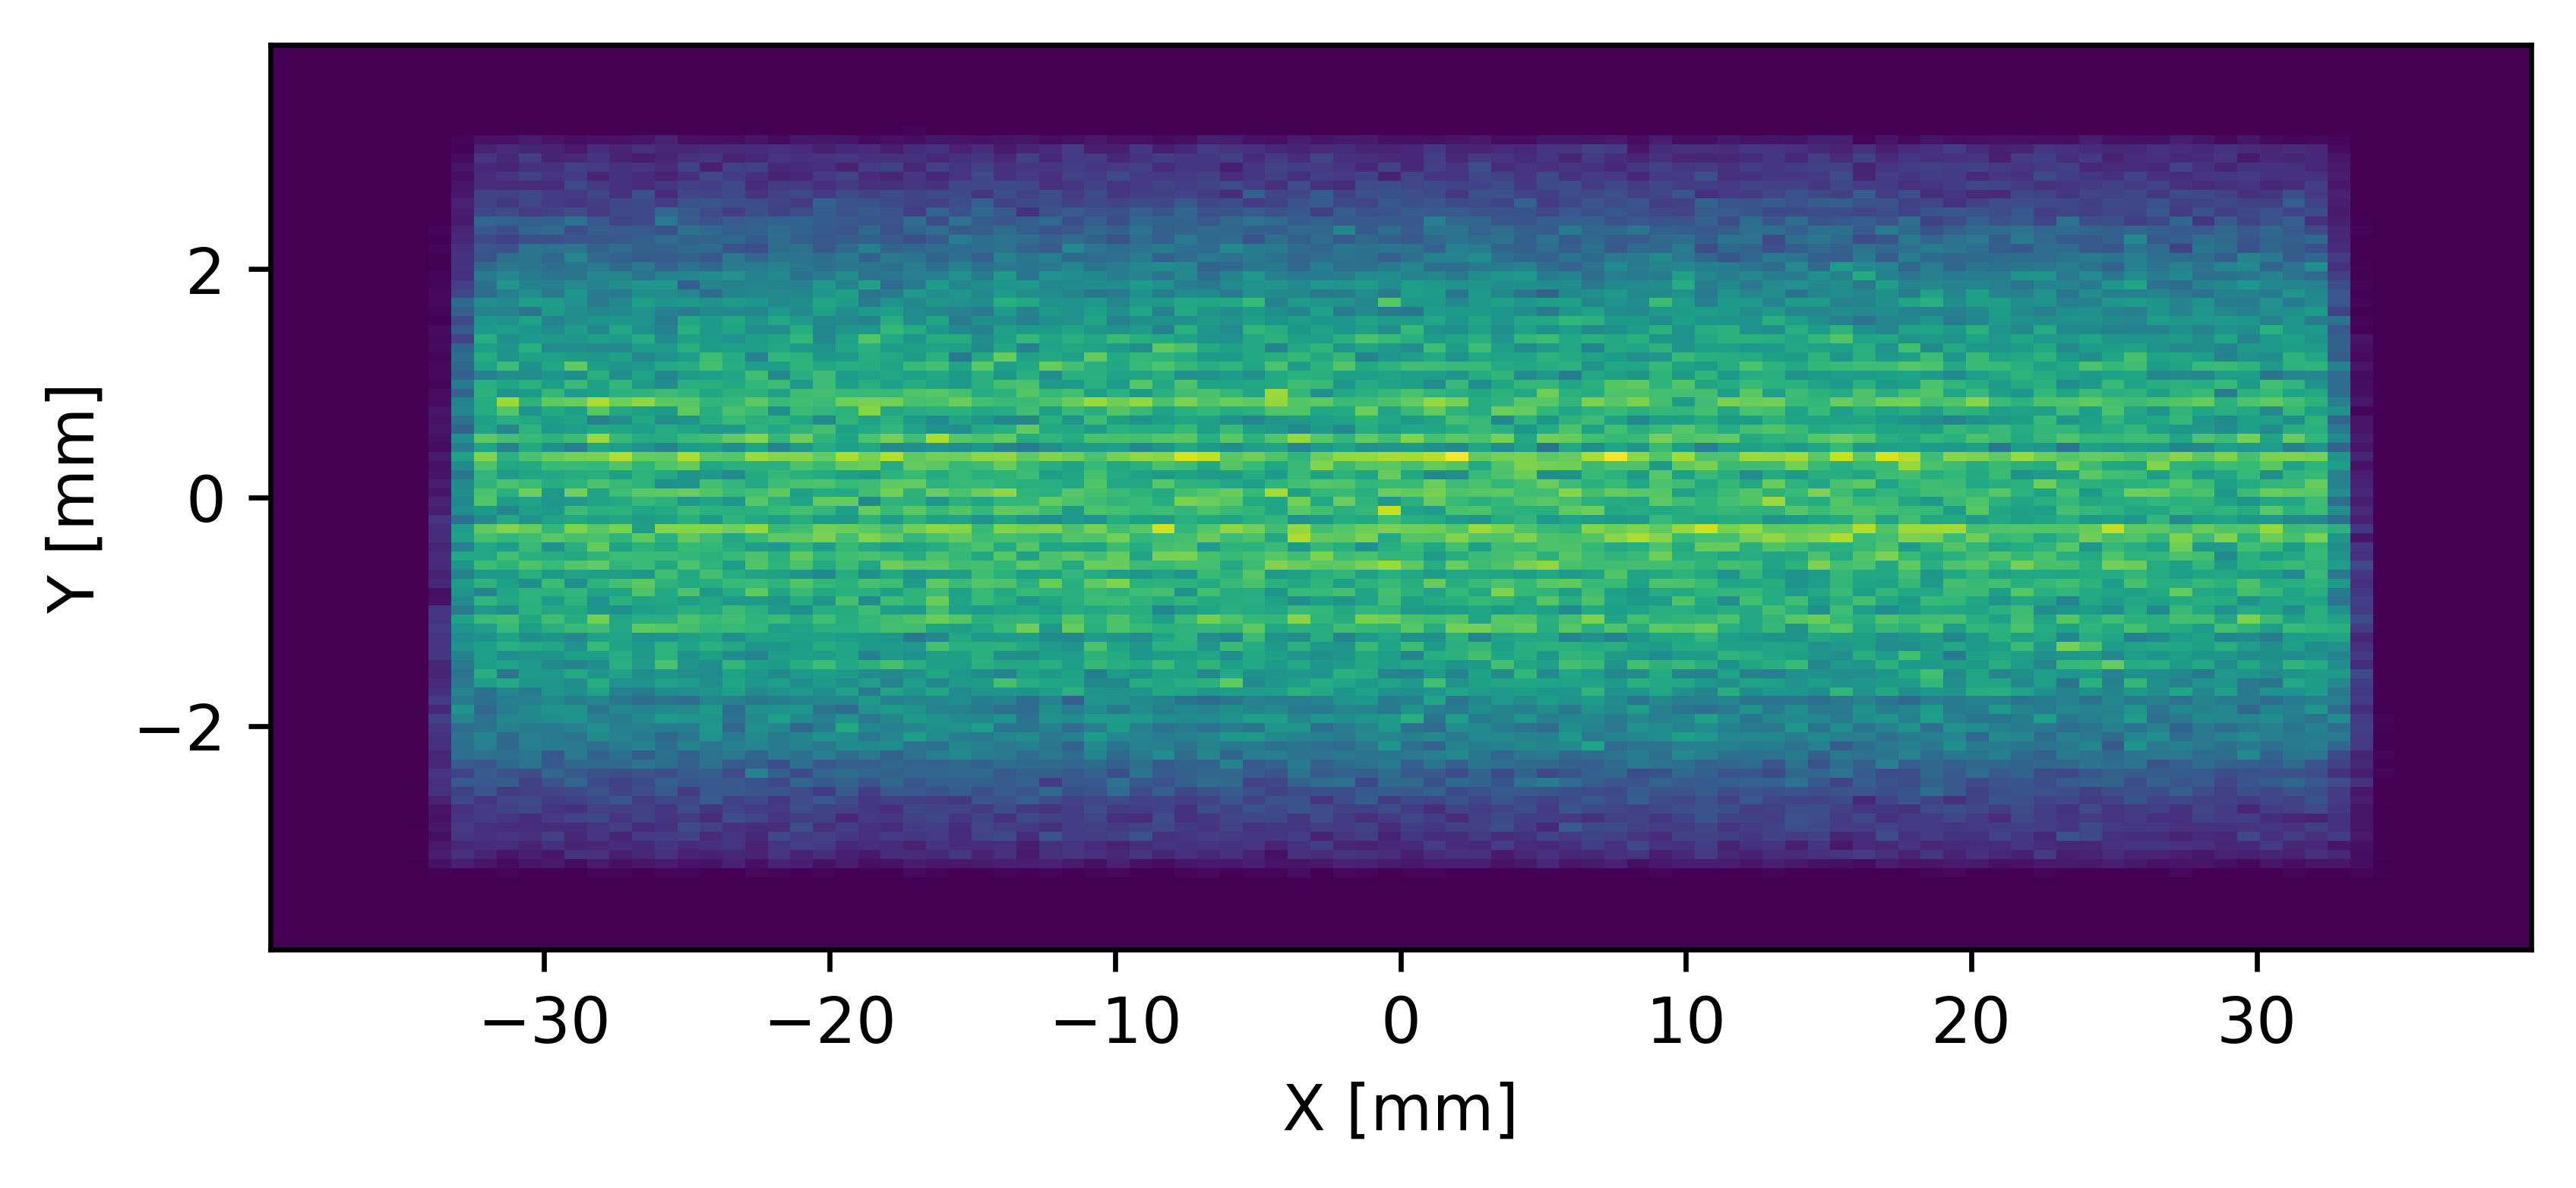
\includegraphics[width=0.85\linewidth]{./../figures/slope_error/WB4C_d30_d-spacing_gradient_45keV_slope_error01urad_ESRFID19PW150.png}
\end{figure}

\begin{figure}[H]
\centering
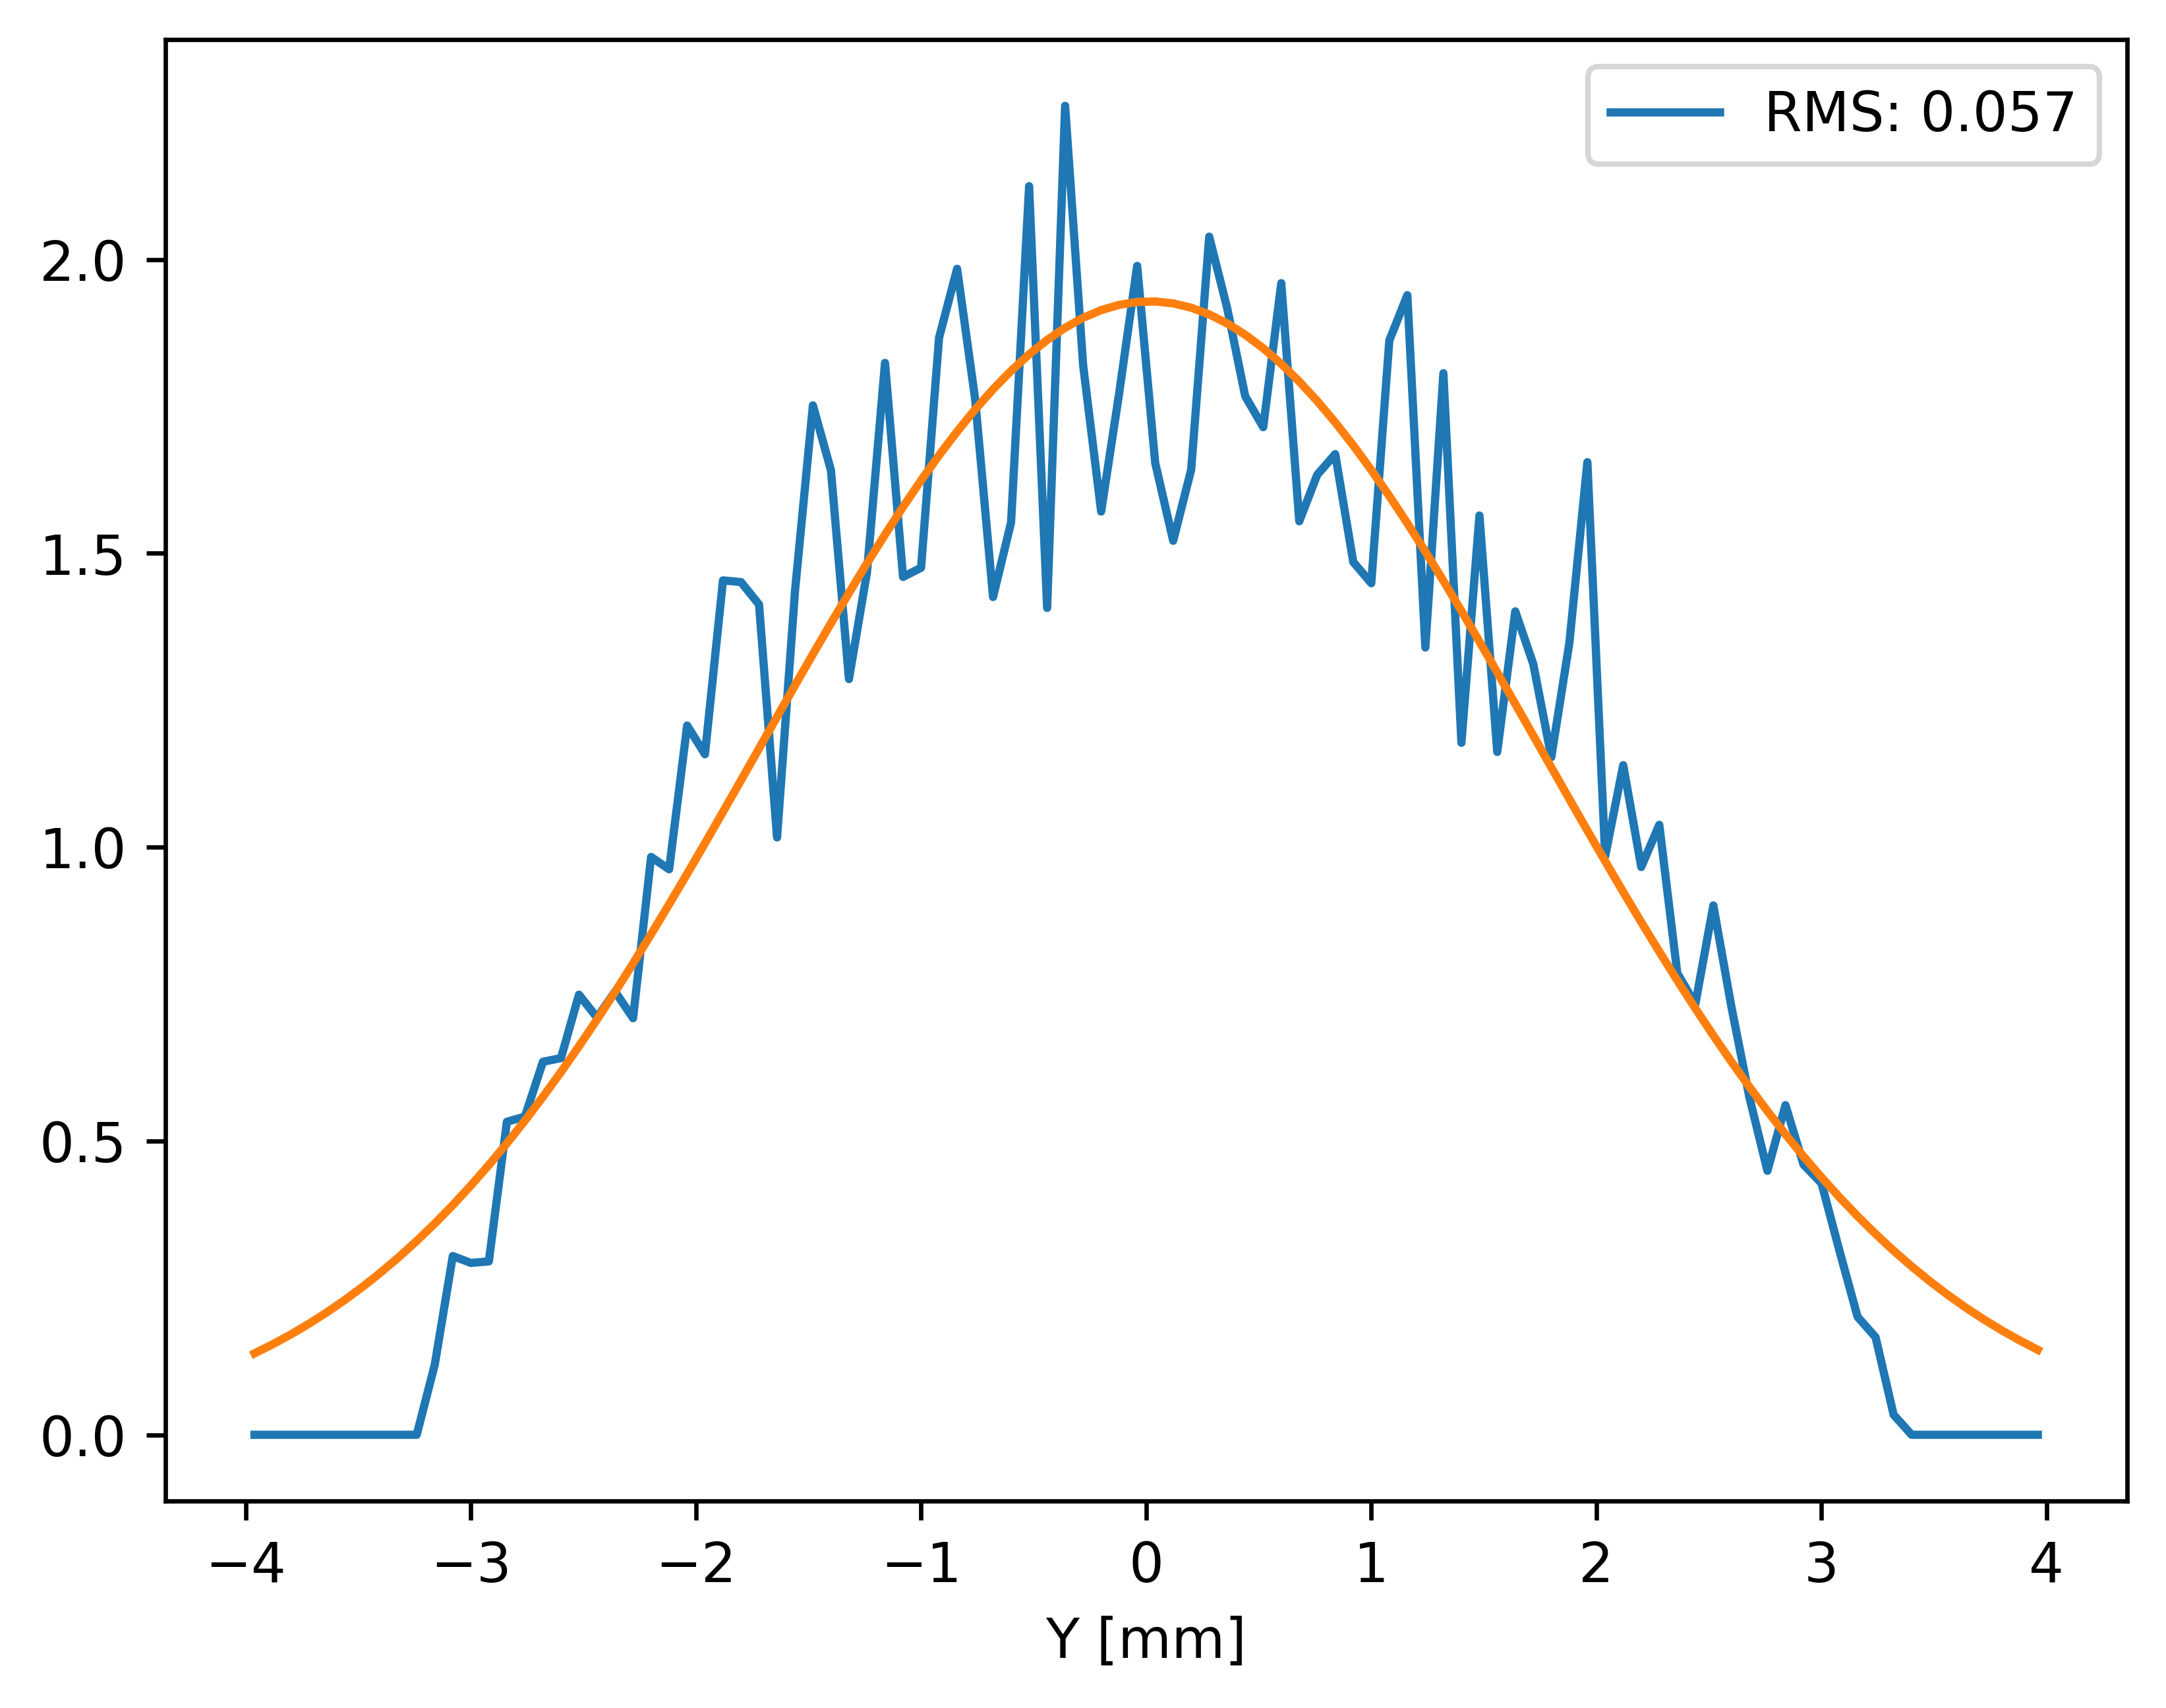
\includegraphics[width=0.85\linewidth]{./../figures/slope_error/WB4C_d30_d-spacing_gradient_45keV_slope_error01urad_ESRFID19PW150_Yprofile.png}
\caption{0.1 urad}
\label{fig:01urad}
\end{figure}

\clearpage
\subsubsection{0.2 urad}
\begin{figure}[H]
\centering
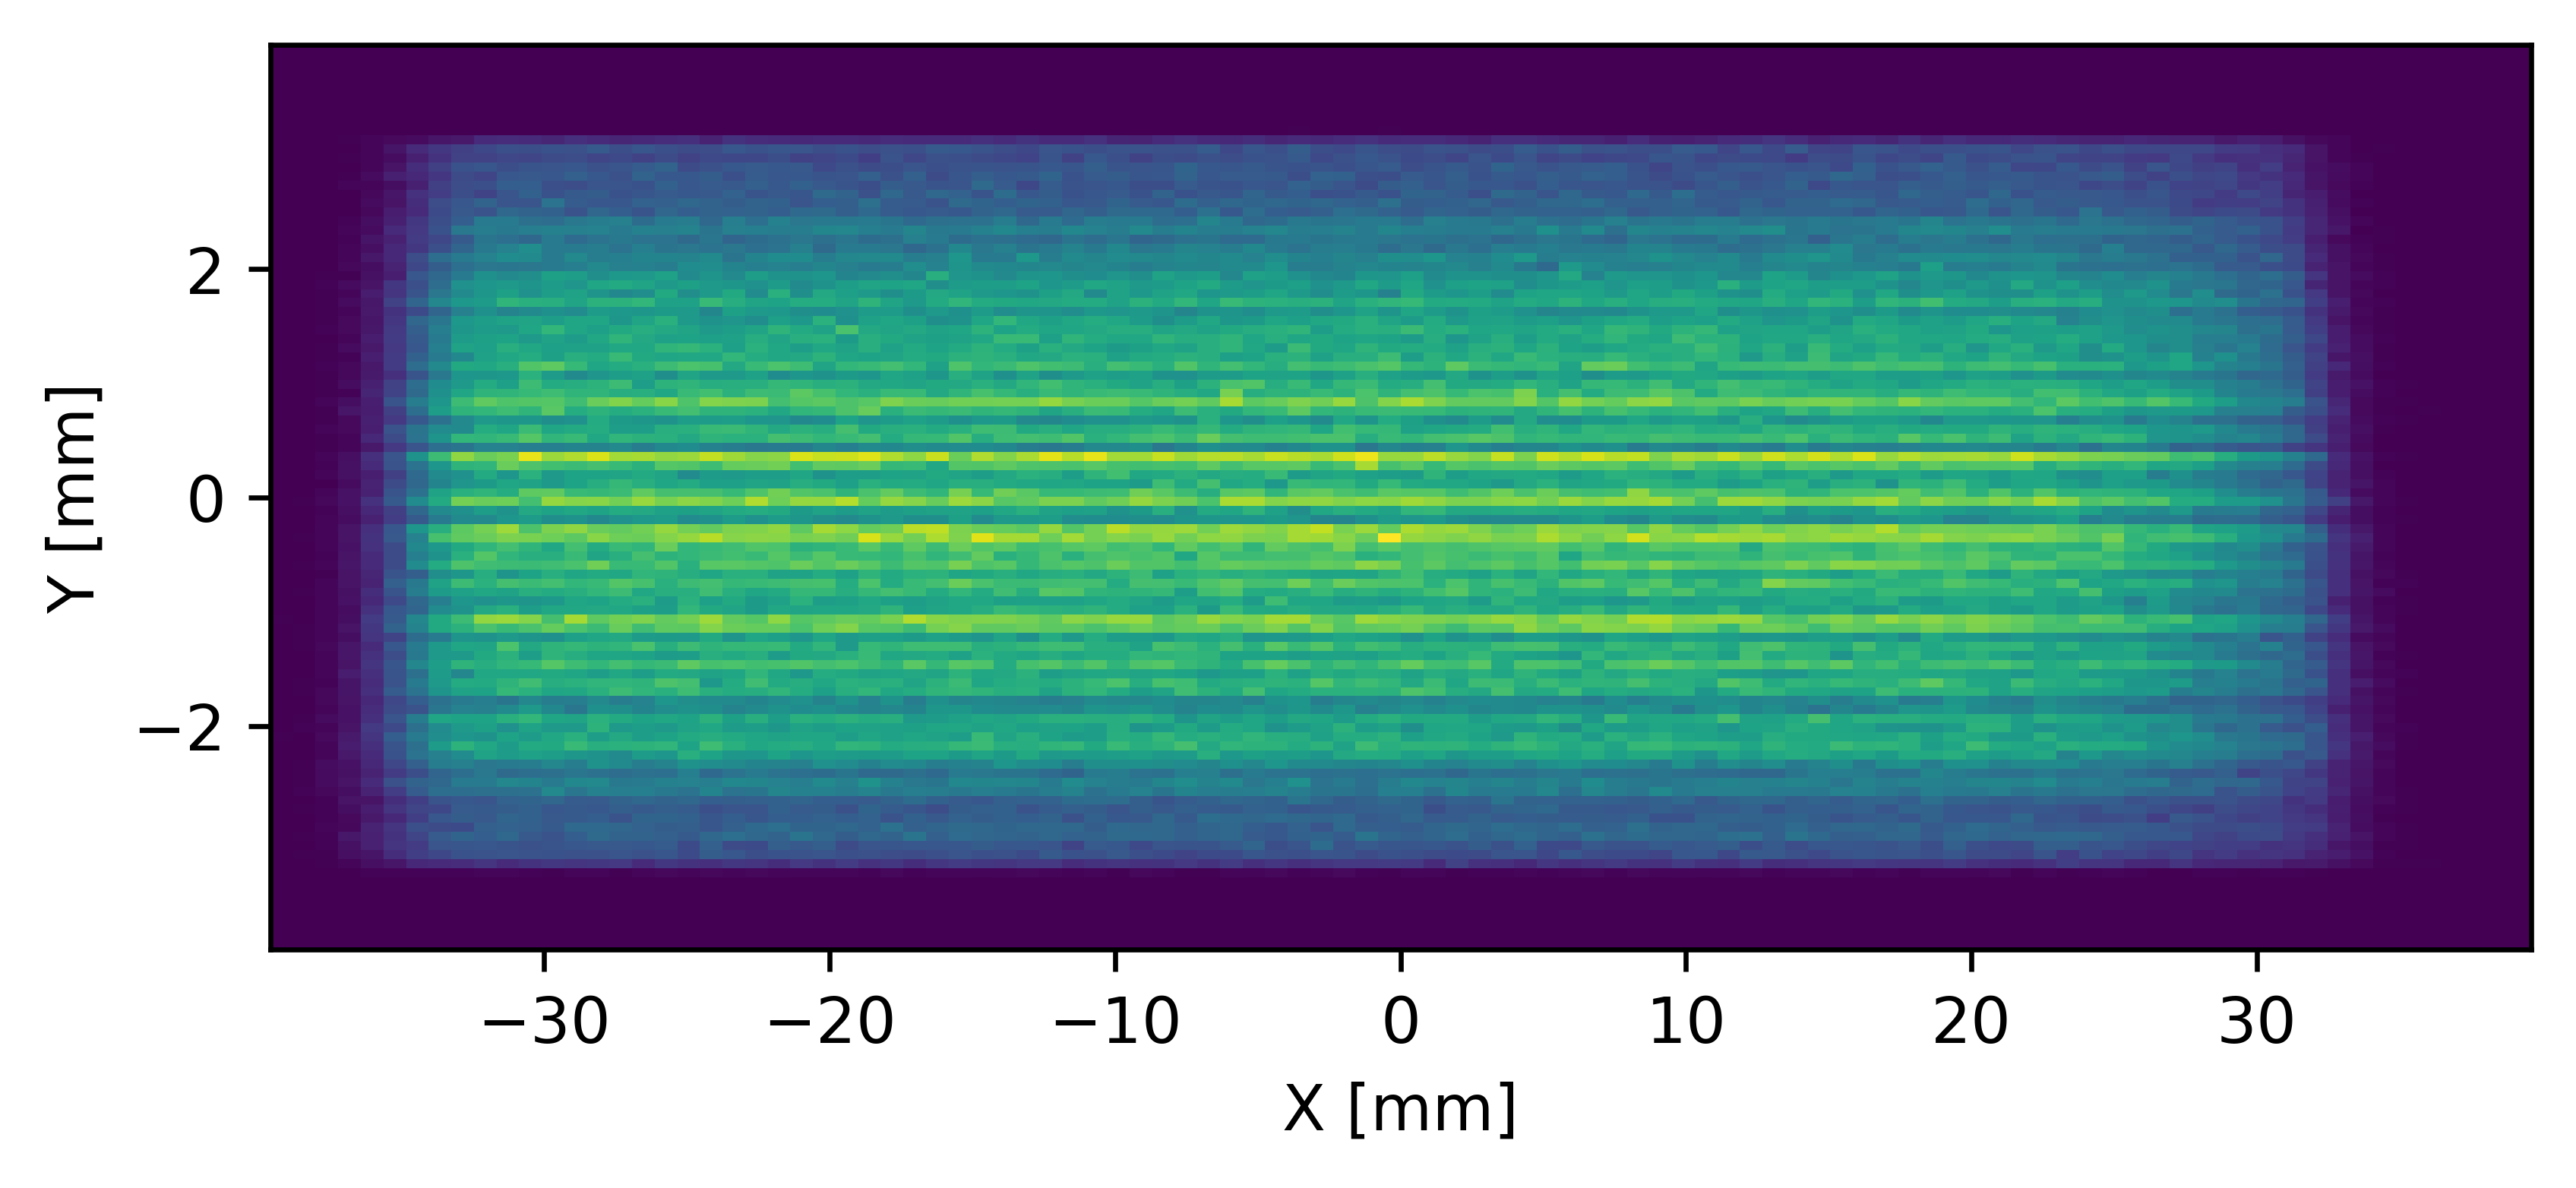
\includegraphics[width=0.9\linewidth]{./../figures/slope_error/WB4C_d30_d-spacing_gradient_45keV_slope_error02urad.png}
\end{figure}

\begin{figure}[H]
\centering
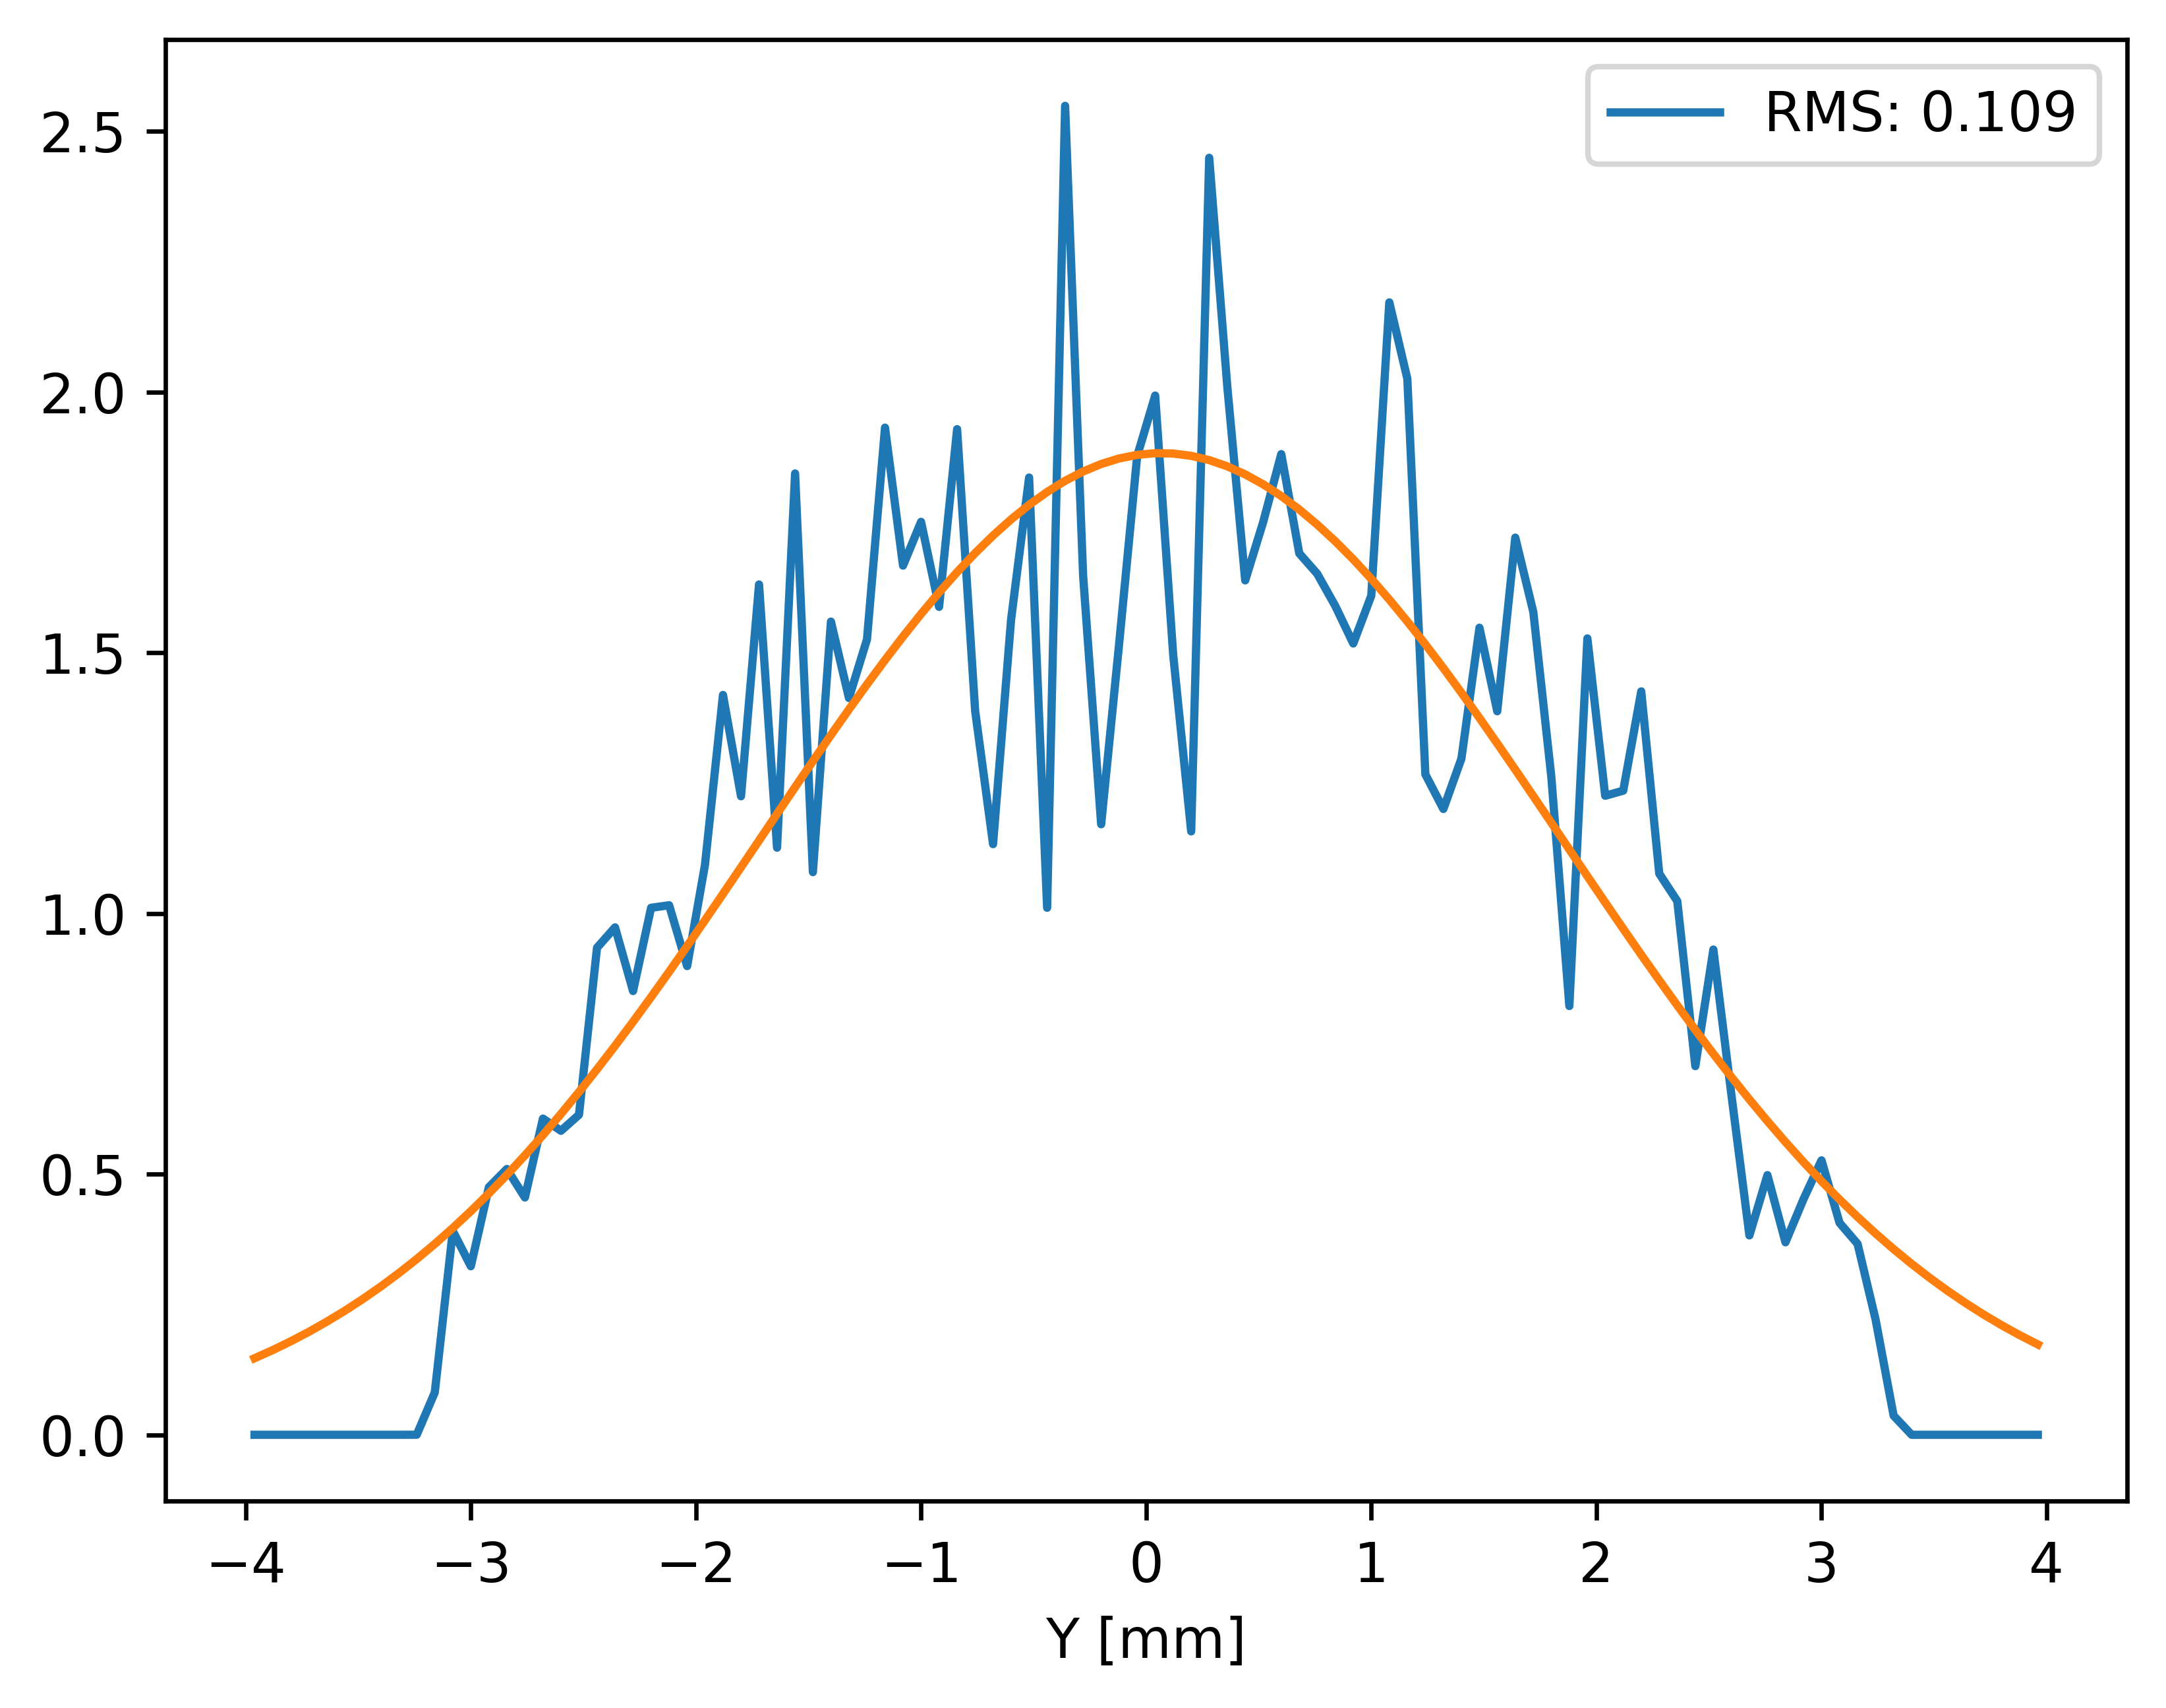
\includegraphics[width=0.9\linewidth]{./../figures/slope_error/WB4C_d30_d-spacing_gradient_45keV_slope_error02urad_ESRFID19PW150_Yprofile.png}
\caption{0.2 urad}
\label{fig:02urad}
\end{figure}

\clearpage
\subsubsection{0.3 urad}
\begin{figure}[H]
\centering
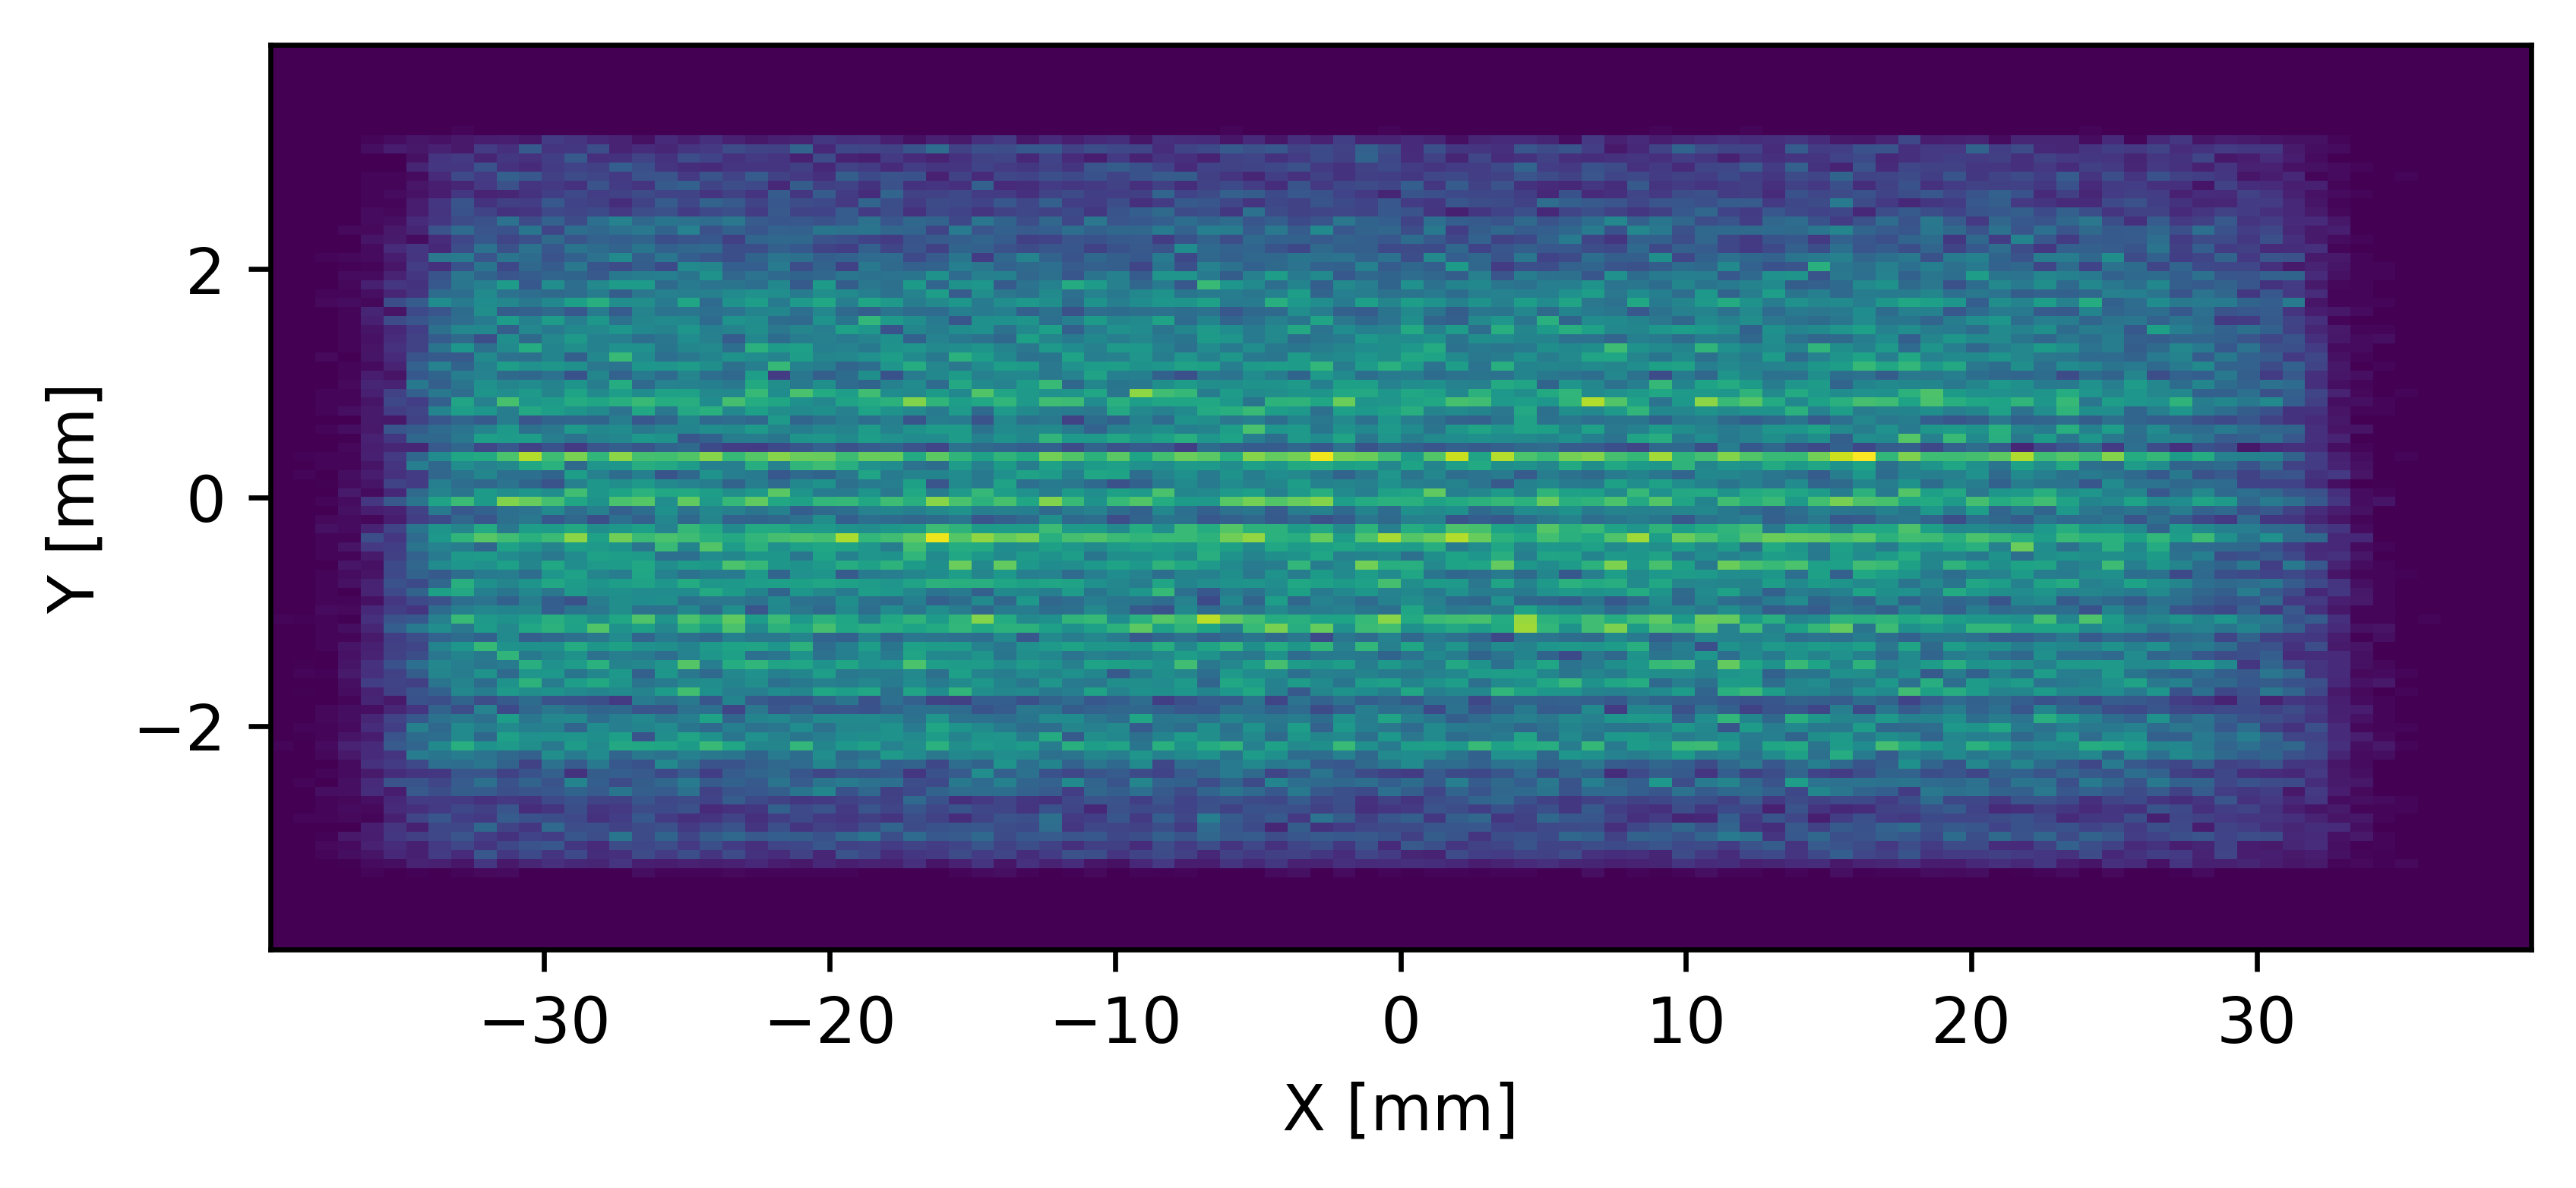
\includegraphics[width=0.9\linewidth]{./../figures/slope_error/WB4C_d30_d-spacing_gradient_45keV_slope_error03urad.png}
\end{figure}

\begin{figure}[H]
\centering
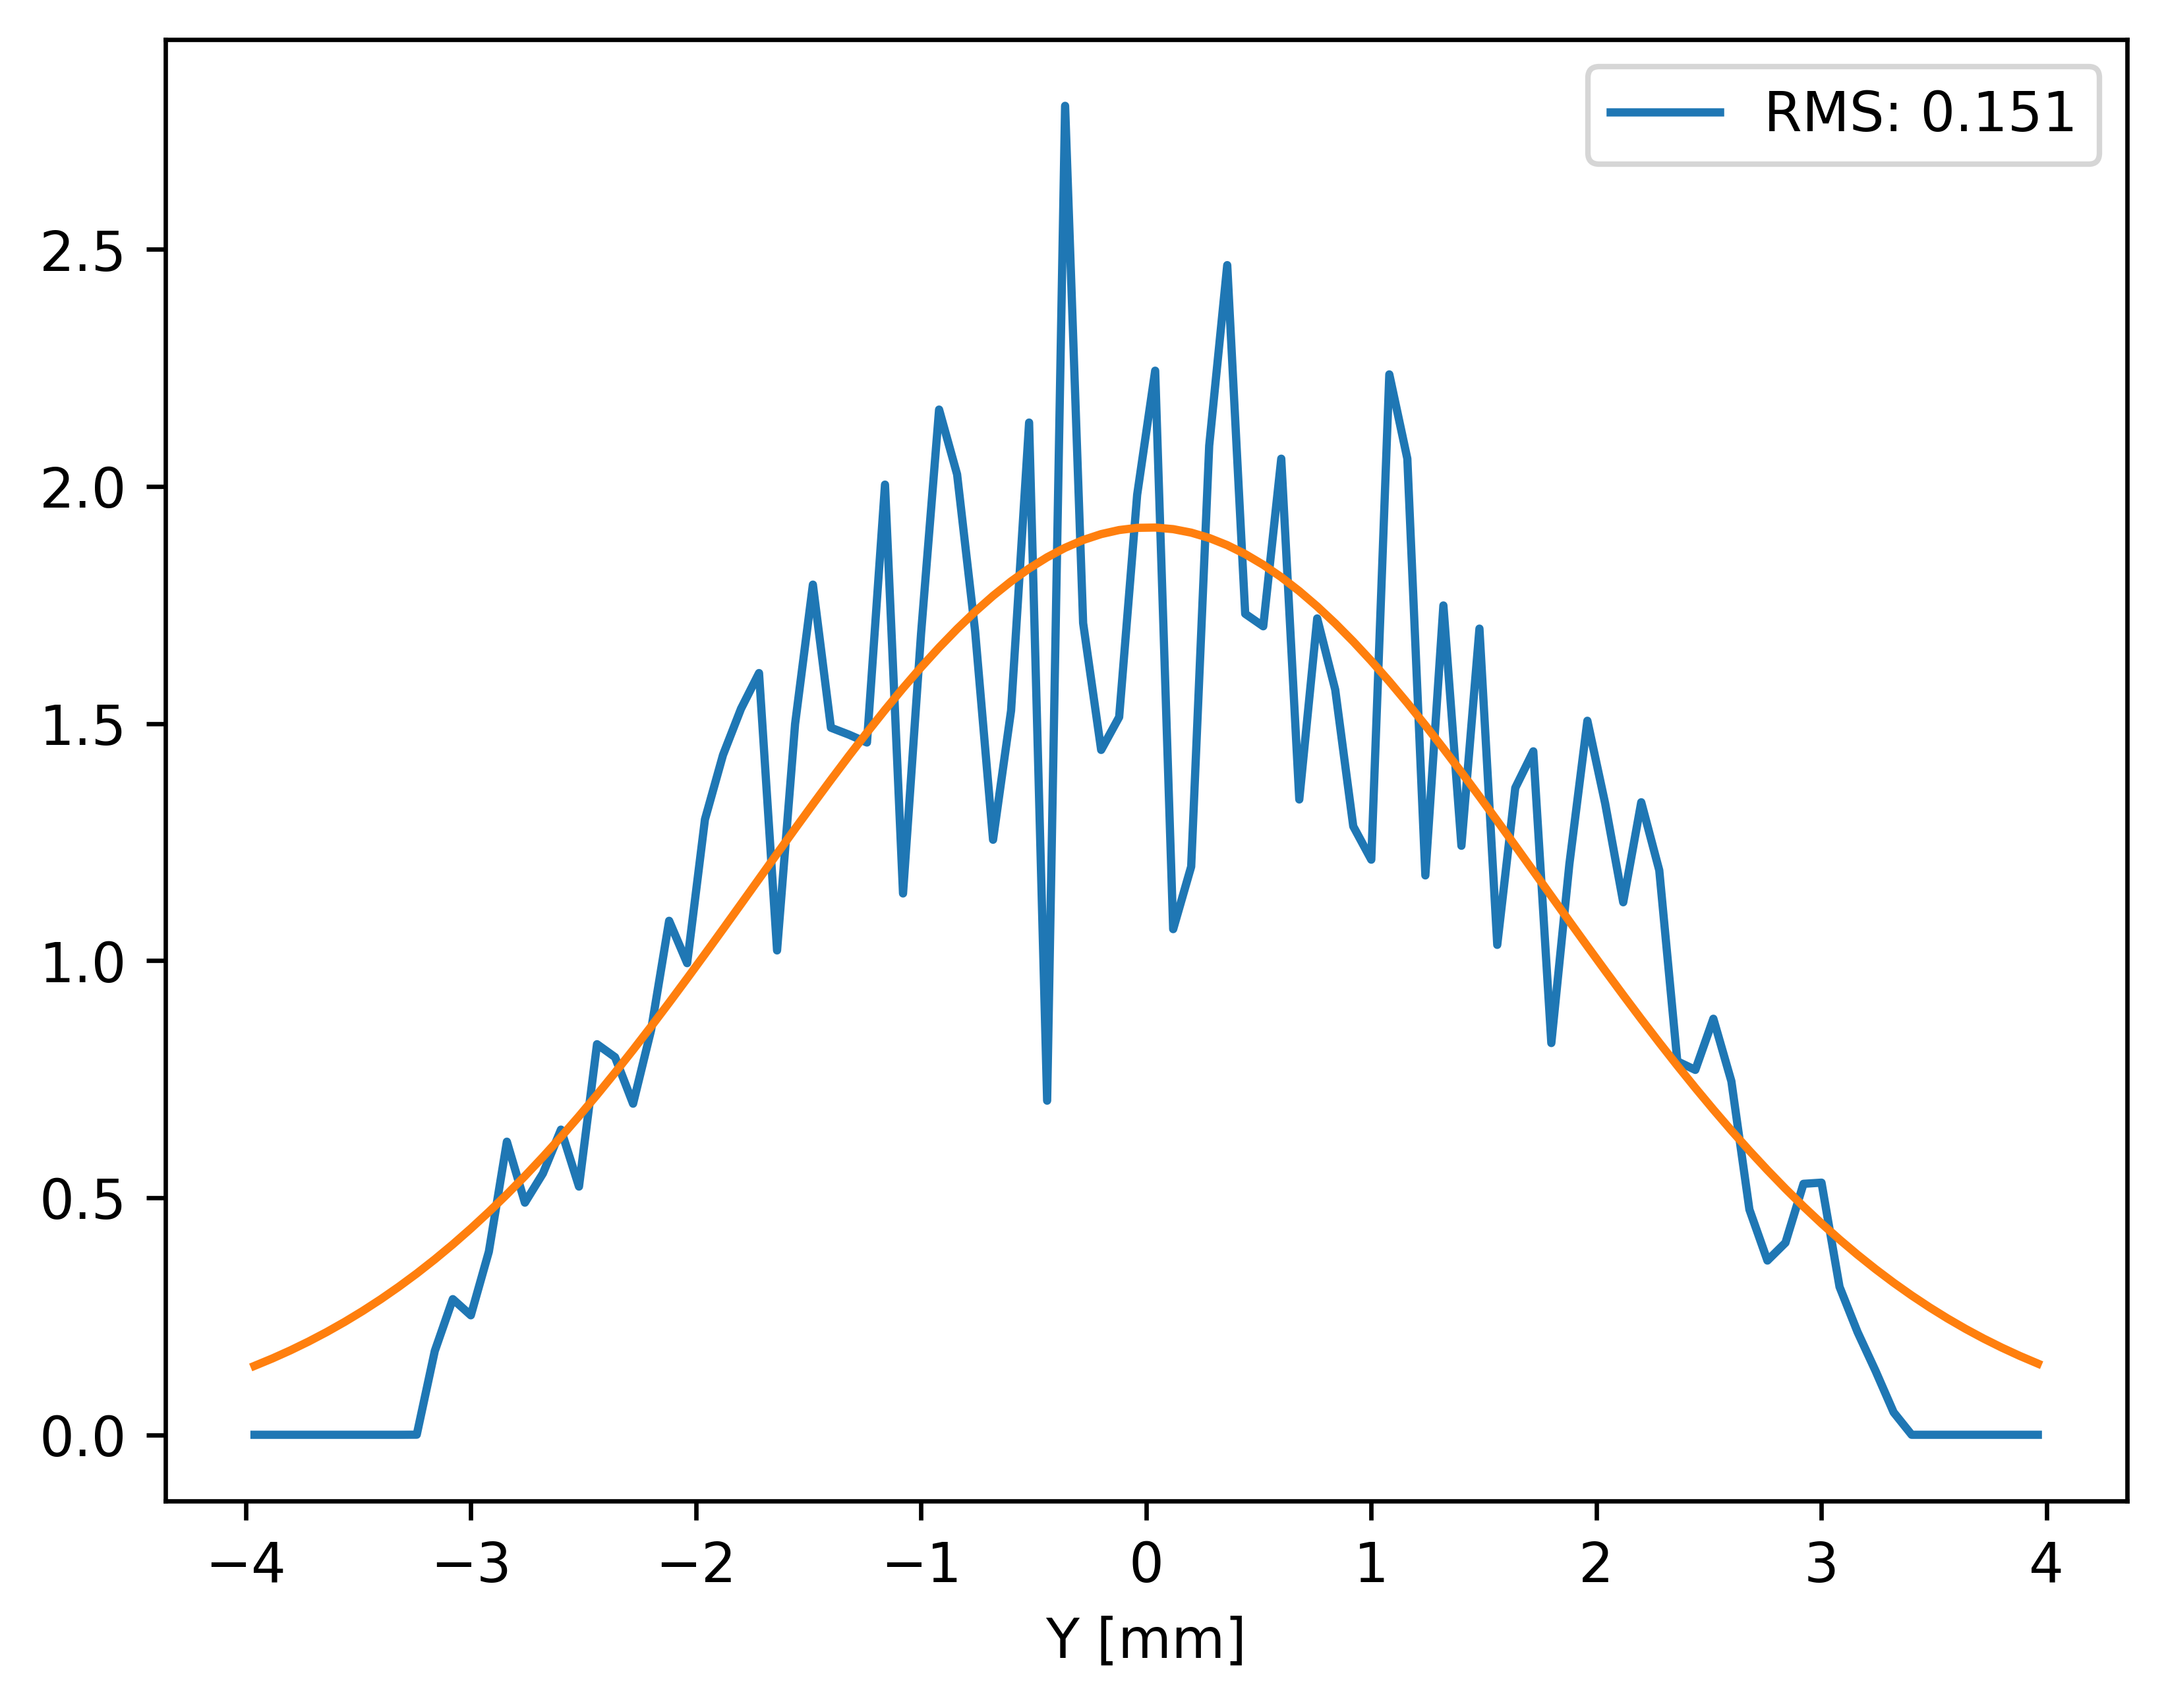
\includegraphics[width=0.9\linewidth]{./../figures/slope_error/WB4C_d30_d-spacing_gradient_45keV_slope_error03urad_ESRFID19PW150_Yprofile.png}
\caption{0.3 urad}
\label{fig:03urad}
\end{figure}

\clearpage
\subsubsection{0.4 urad}
\begin{figure}[H]
\centering
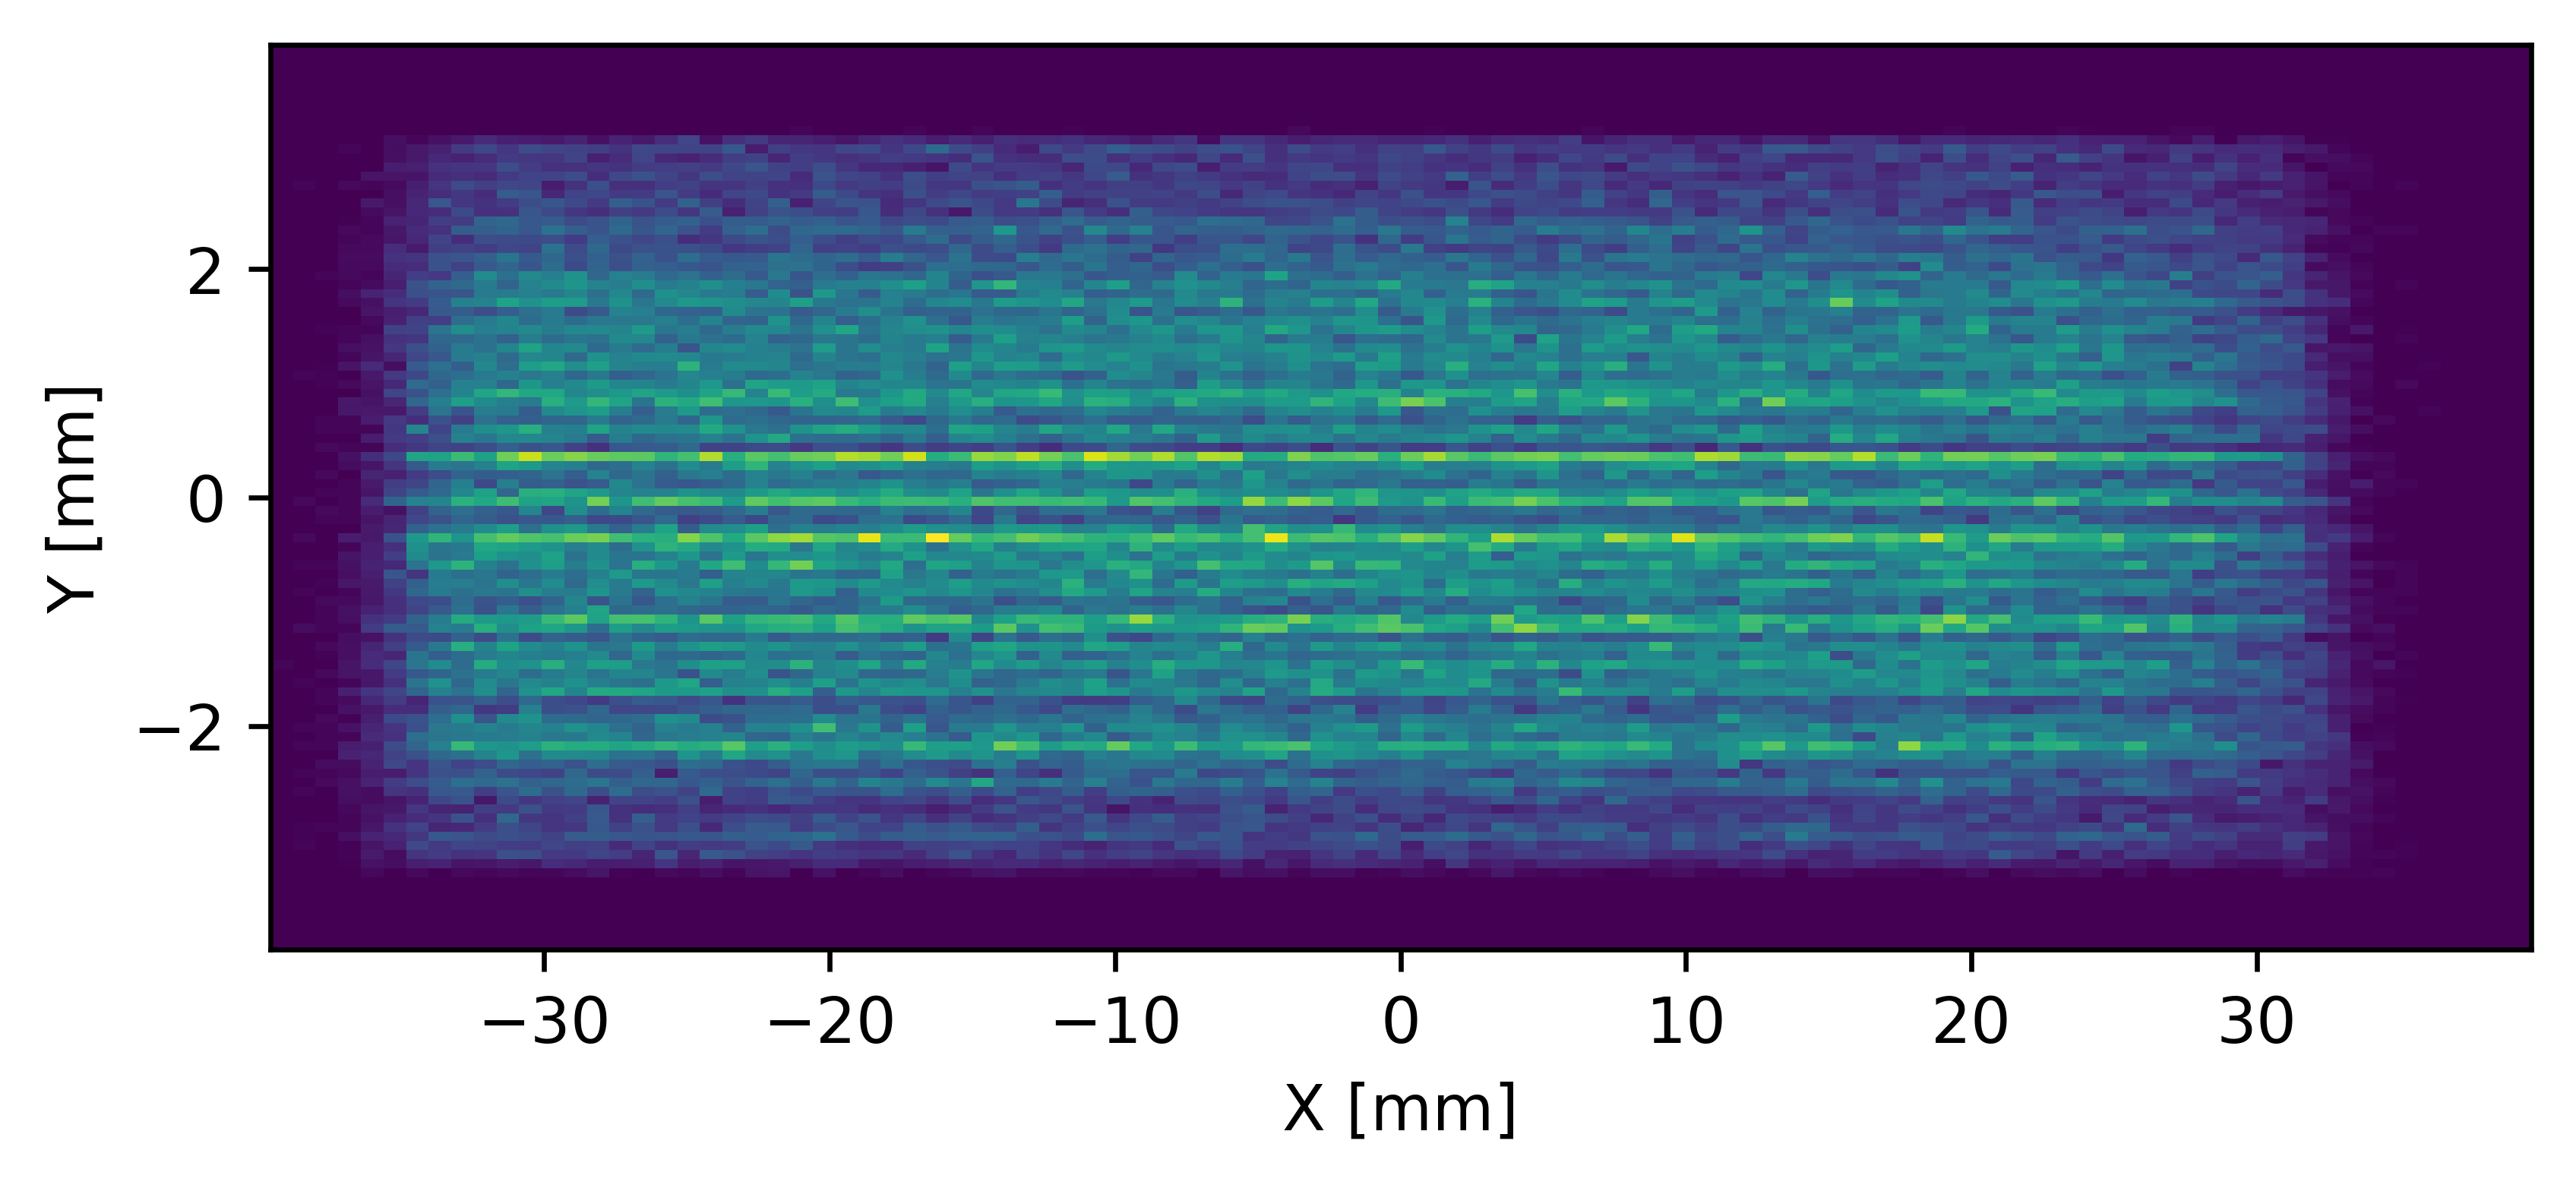
\includegraphics[width=0.9\linewidth]{./../figures/slope_error/WB4C_d30_d-spacing_gradient_45keV_slope_error04urad.png}
\end{figure}

\begin{figure}[H]
\centering
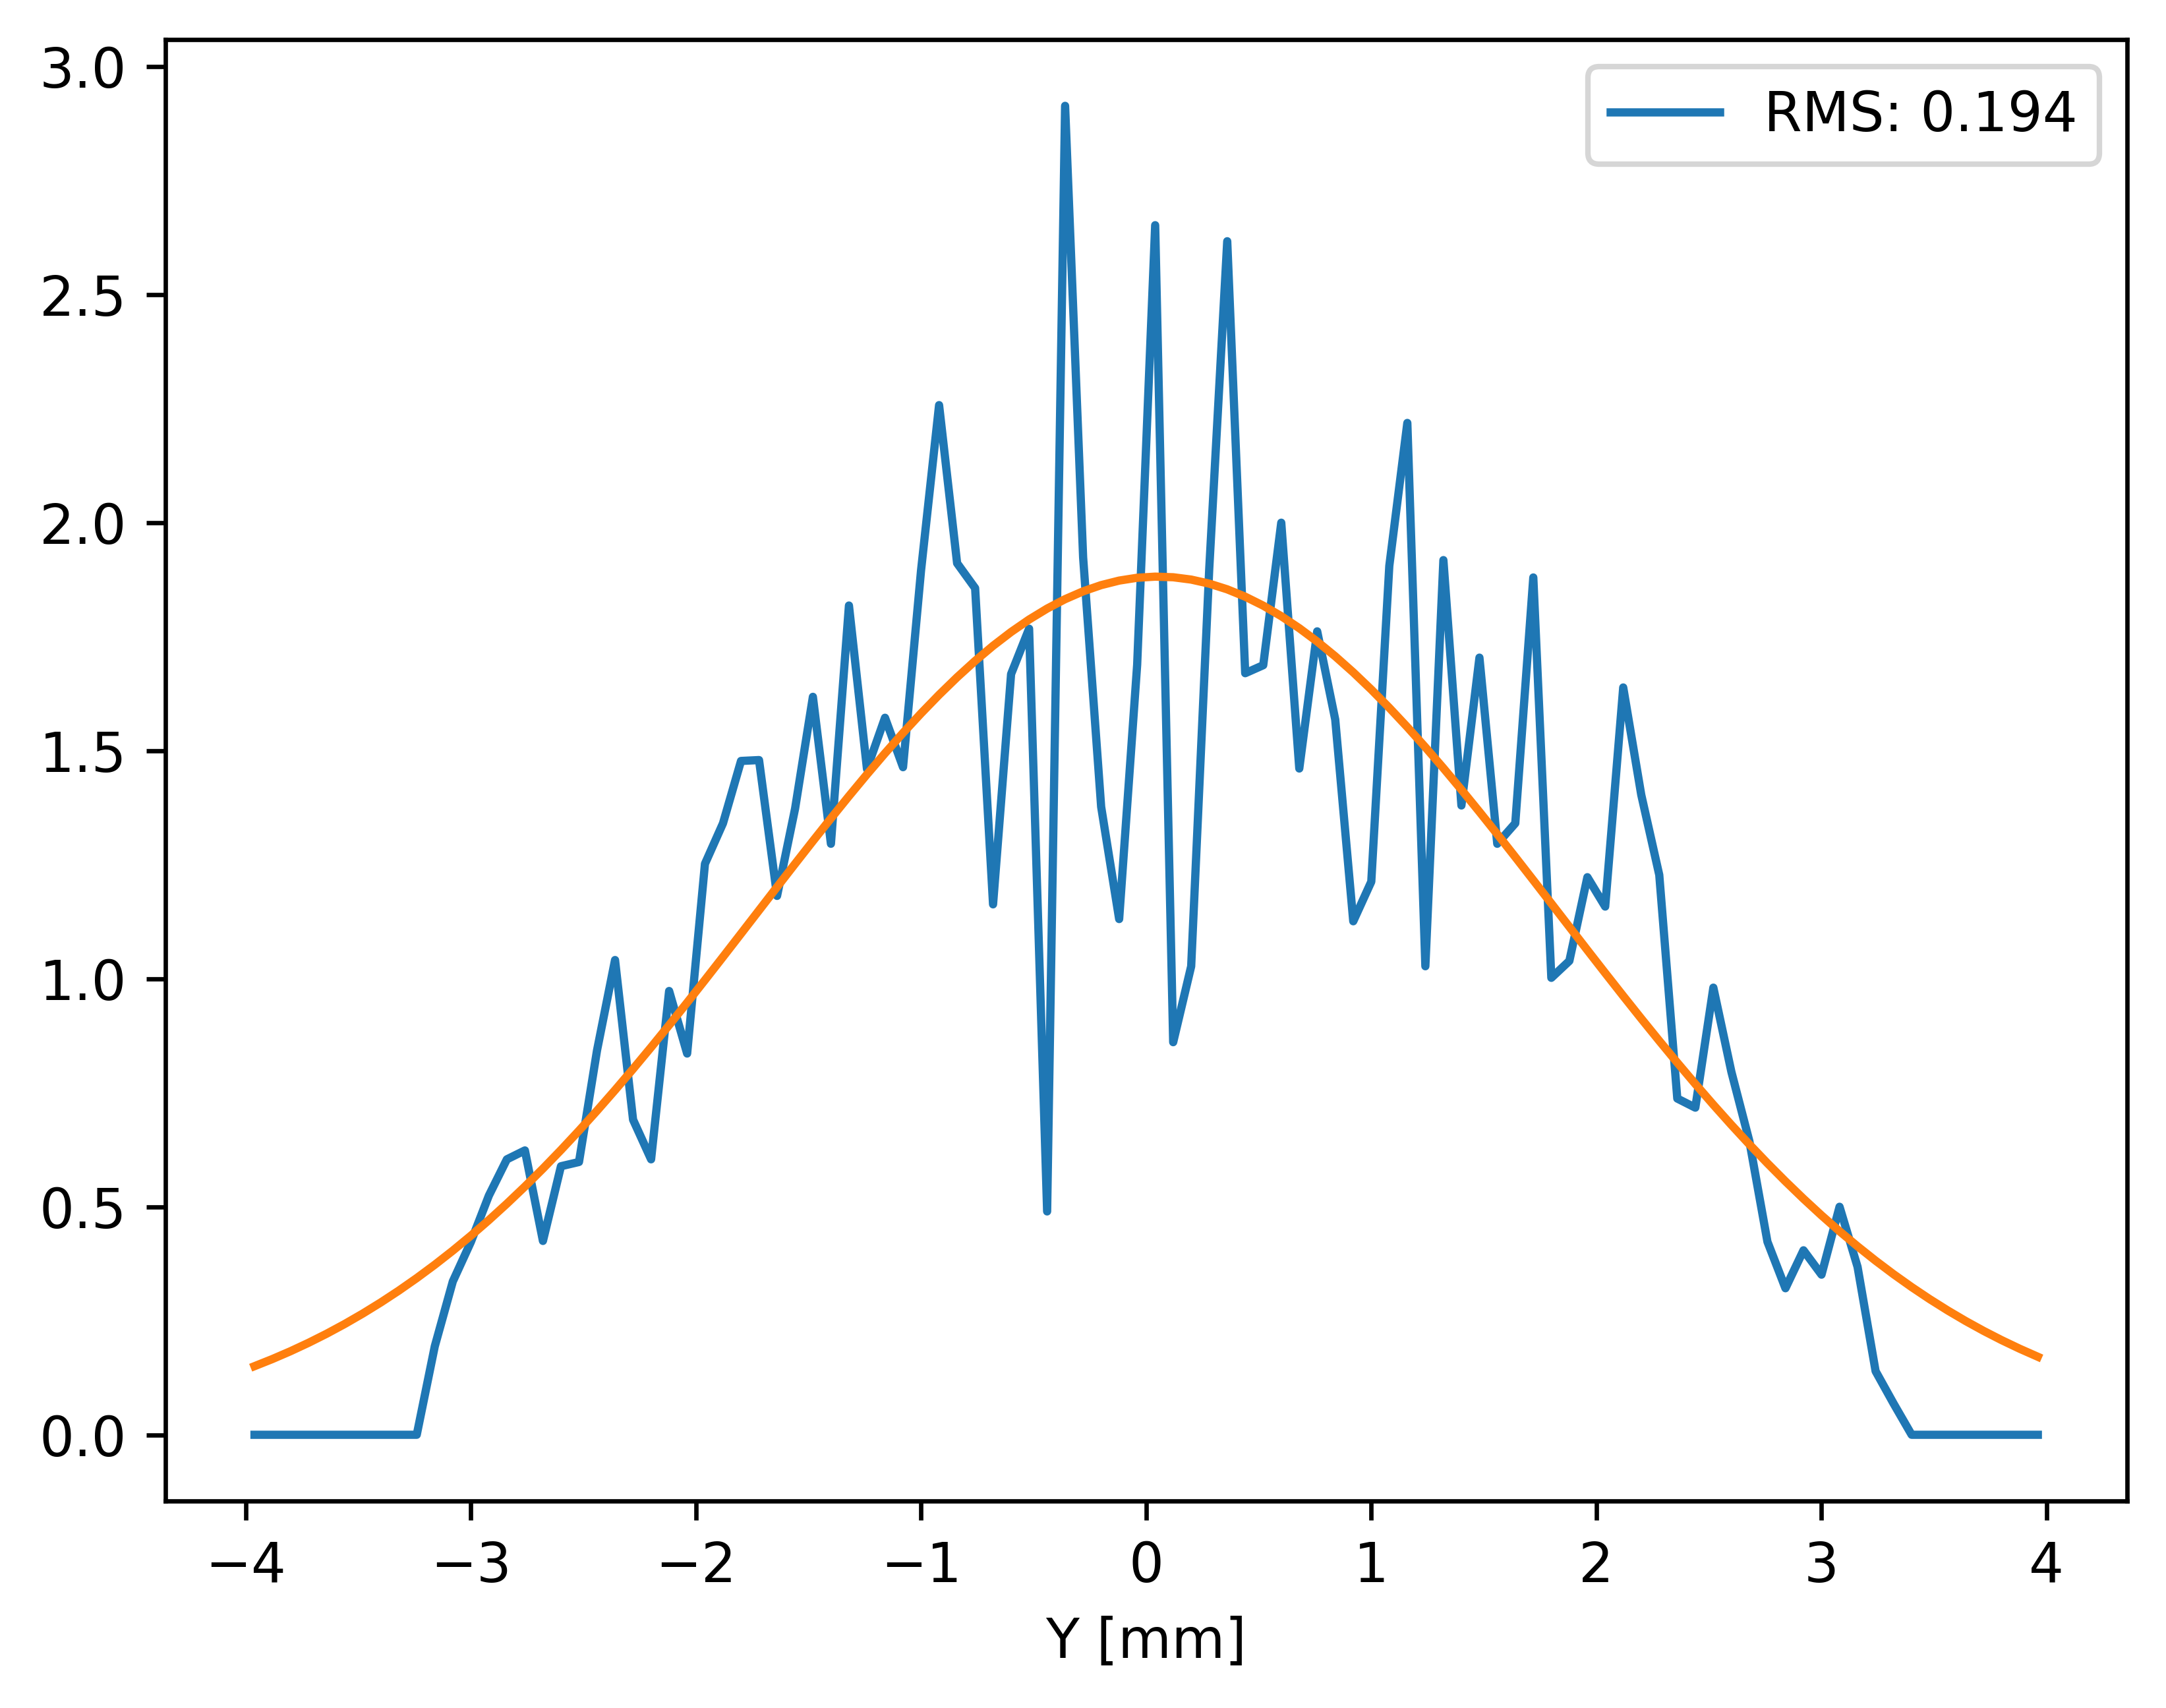
\includegraphics[width=0.9\linewidth]{./../figures/slope_error/WB4C_d30_d-spacing_gradient_45keV_slope_error04urad_ESRFID19PW150_Yprofile.png}
\caption{0.4 urad}
\label{fig:04urad}
\end{figure}

\clearpage
\subsubsection{0.5 urad}
\begin{figure}[H]
\centering
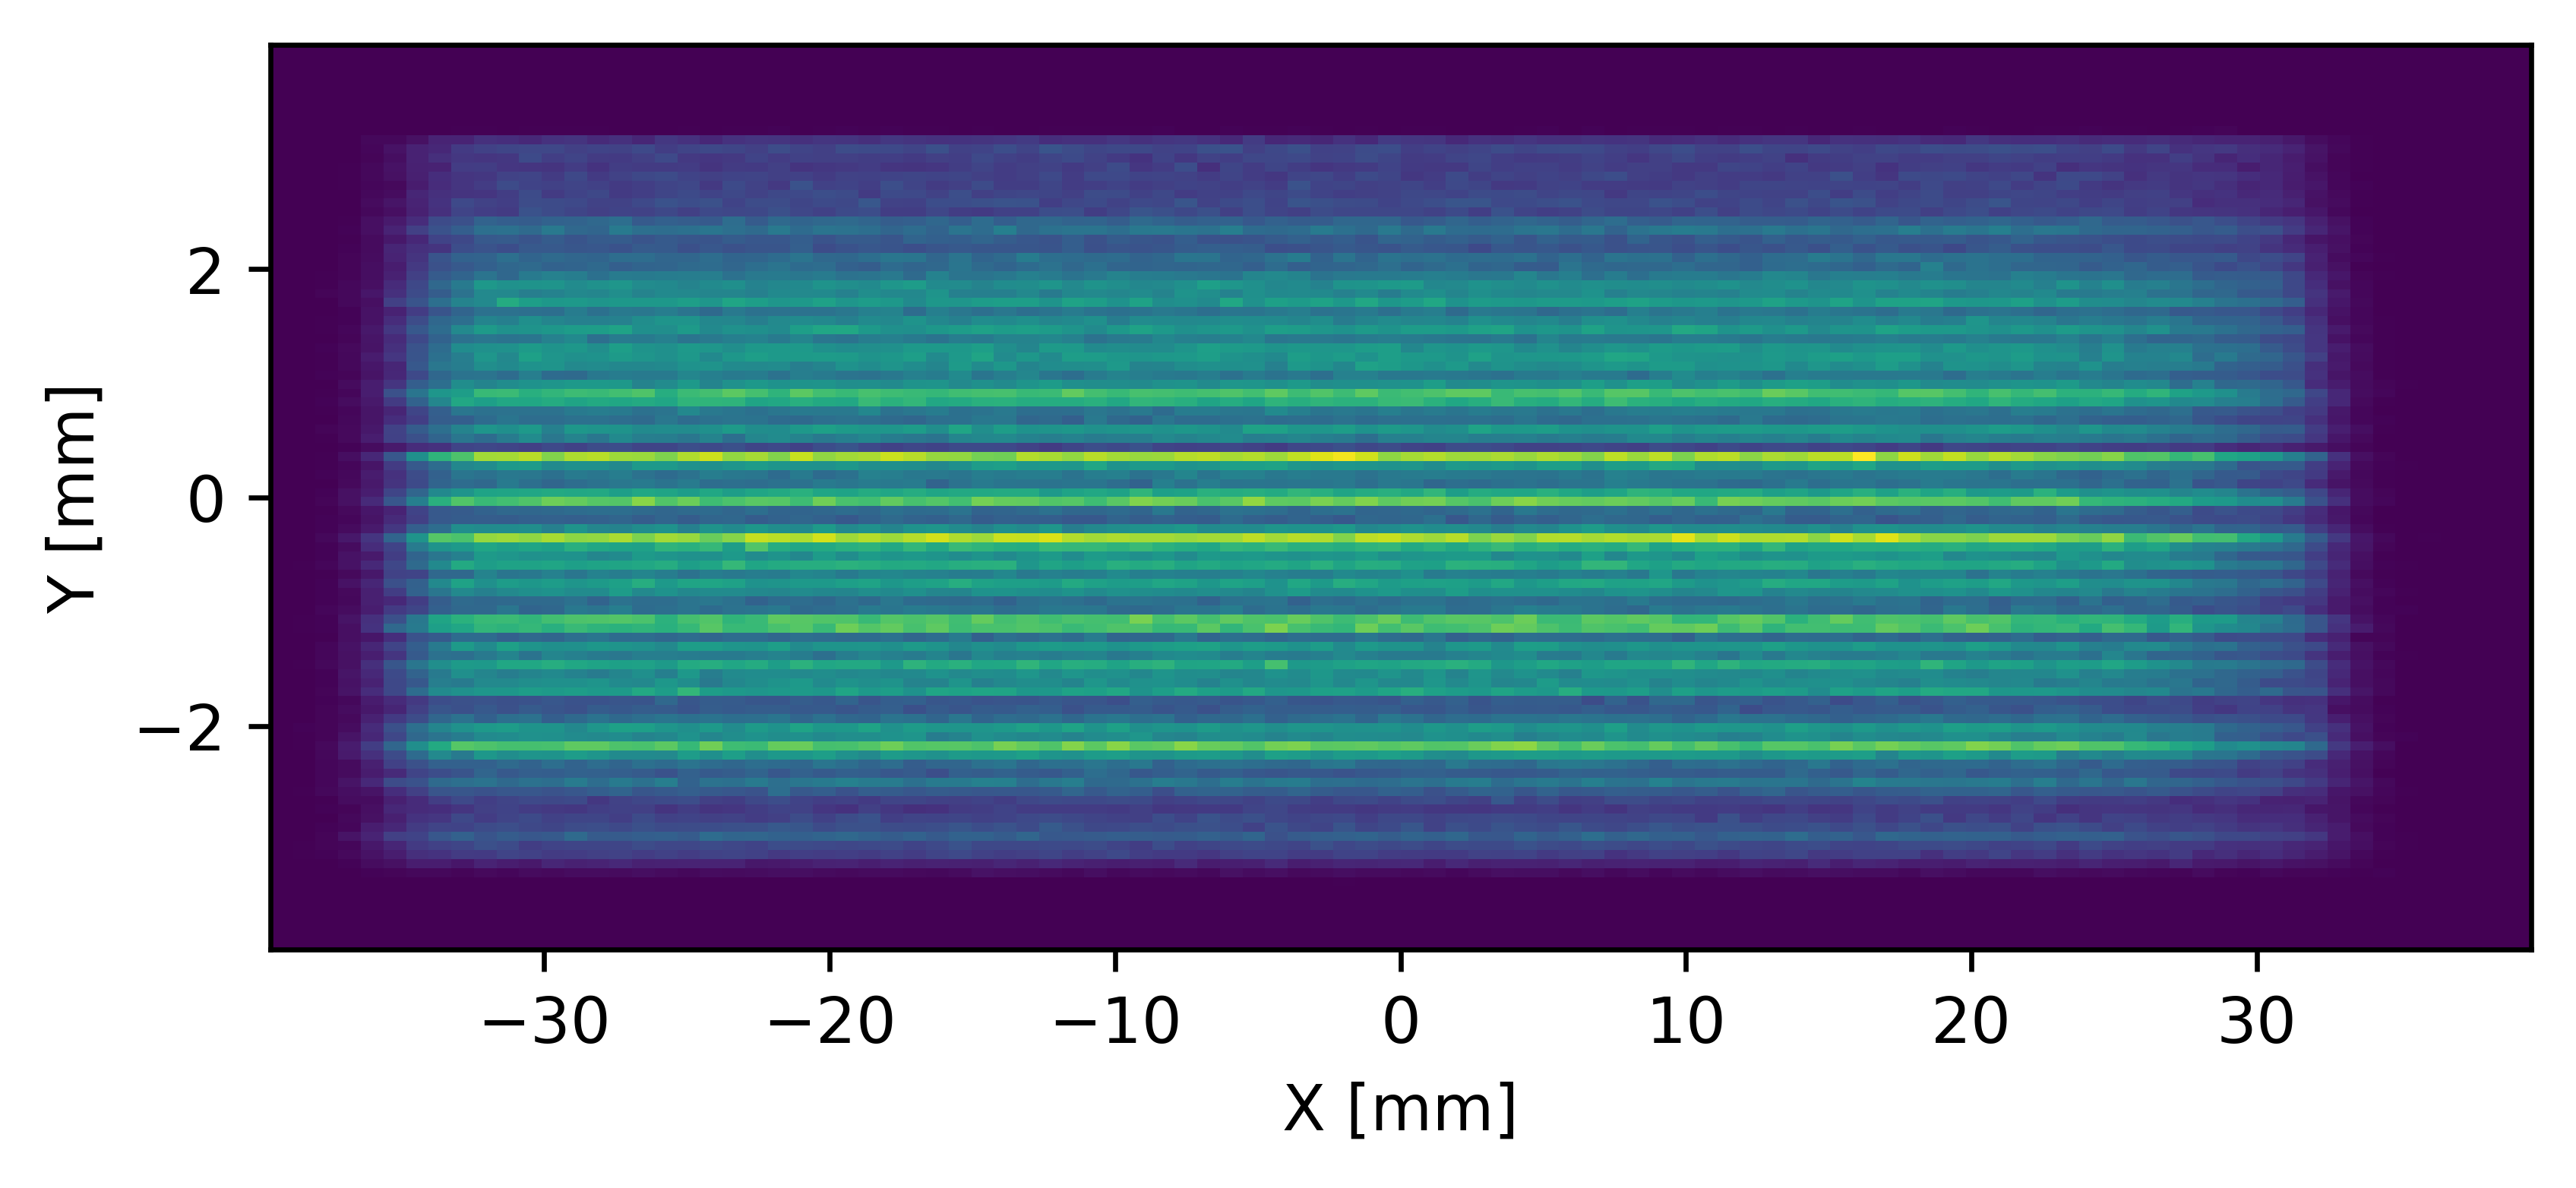
\includegraphics[width=0.9\linewidth]{./../figures/slope_error/WB4C_d30_d-spacing_gradient_45keV_slope_error05urad.png}
\end{figure}

\begin{figure}[H]
\centering
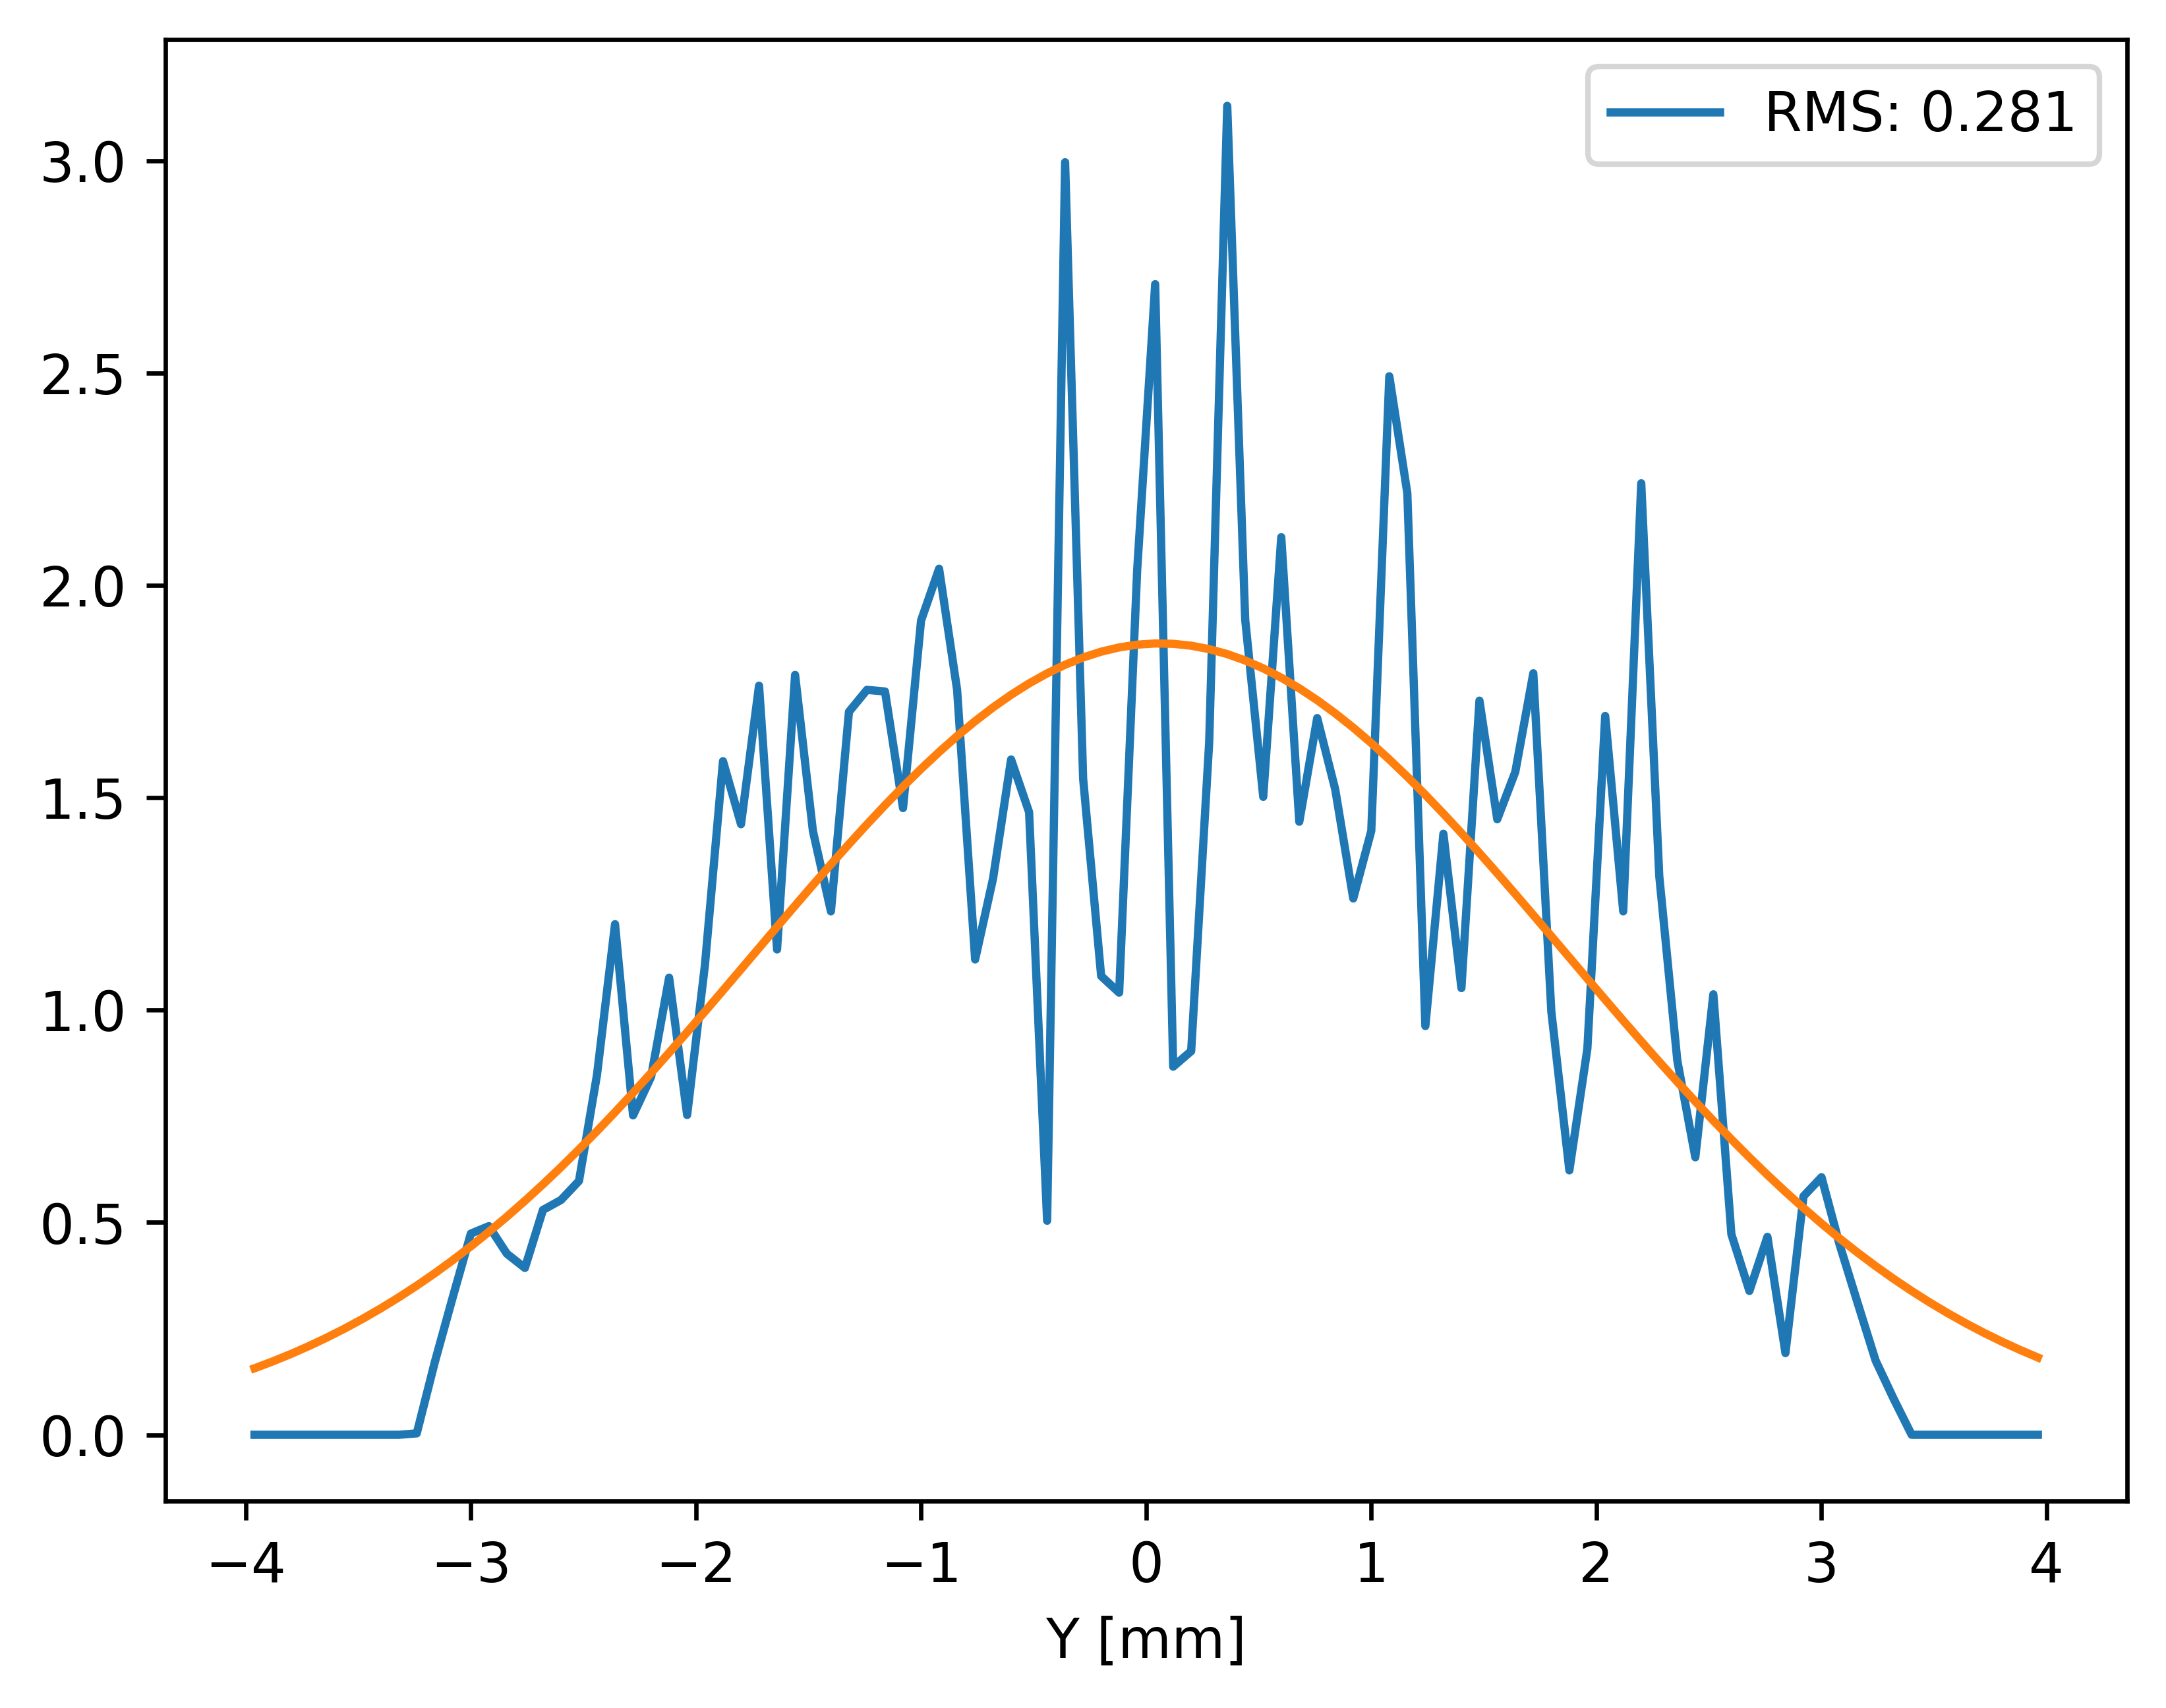
\includegraphics[width=0.9\linewidth]{./../figures/slope_error/WB4C_d30_d-spacing_gradient_45keV_slope_error05urad_ESRFID19PW150_Yprofile.png}
\caption{0.5 urad}
\label{fig:05urad}
\end{figure}


%%%%%%%%%%%%%%%%%%%%%%%%%%%%%%%%%%%%%%%%%%%%%%%%%%%%%%%%%%%%%%%%%%%%%%%%%%%%%%%%%%%%
\clearpage
\subsection{Thermal stability}
The thermal stability of ML1 should be verified with FEA simulations considering the white beam colliding with the mirror at the maximum Bragg angle allowed by the Bragg stage motorization (34.9 mrad). The thermal stability of the cooled mask in front of the ML1 profile shall be also verified.\\

The power density profile at 15.165 m from source is shown in Figure \ref{fig:power_profile_ML1}. Raw data can be found in the \powerprofilesurl. \\
\begin{figure}[ht]
\centering
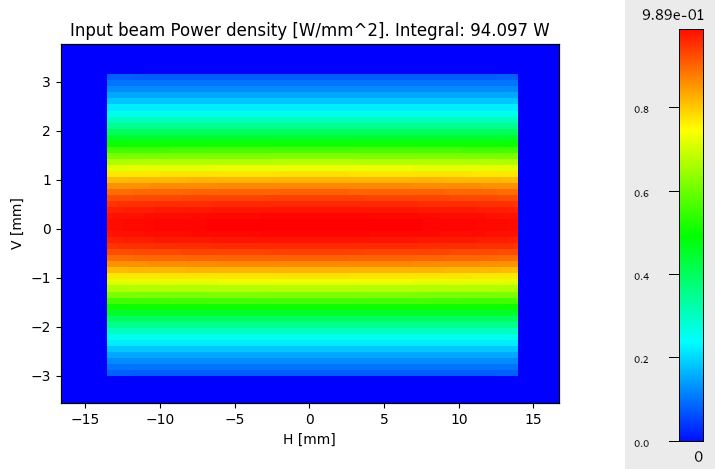
\includegraphics[width=0.8\textwidth]{./../../power_profiles/power_profile_ML1.png}
\caption{\label{fig:power_profile_ML1} Power density profile at 15.165 m from source (center position of ML1).}
\end{figure}

% \bibliography{references}
% \bibliographystyle{plain}

\end{document}
